% Options for packages loaded elsewhere
% Options for packages loaded elsewhere
\PassOptionsToPackage{unicode}{hyperref}
\PassOptionsToPackage{hyphens}{url}
\PassOptionsToPackage{dvipsnames,svgnames,x11names}{xcolor}
%
\documentclass[
  letterpaper,
  DIV=11,
  numbers=noendperiod]{scrreprt}
\usepackage{xcolor}
\usepackage{amsmath,amssymb}
\setcounter{secnumdepth}{5}
\usepackage{iftex}
\ifPDFTeX
  \usepackage[T1]{fontenc}
  \usepackage[utf8]{inputenc}
  \usepackage{textcomp} % provide euro and other symbols
\else % if luatex or xetex
  \usepackage{unicode-math} % this also loads fontspec
  \defaultfontfeatures{Scale=MatchLowercase}
  \defaultfontfeatures[\rmfamily]{Ligatures=TeX,Scale=1}
\fi
\usepackage{lmodern}
\ifPDFTeX\else
  % xetex/luatex font selection
\fi
% Use upquote if available, for straight quotes in verbatim environments
\IfFileExists{upquote.sty}{\usepackage{upquote}}{}
\IfFileExists{microtype.sty}{% use microtype if available
  \usepackage[]{microtype}
  \UseMicrotypeSet[protrusion]{basicmath} % disable protrusion for tt fonts
}{}
\makeatletter
\@ifundefined{KOMAClassName}{% if non-KOMA class
  \IfFileExists{parskip.sty}{%
    \usepackage{parskip}
  }{% else
    \setlength{\parindent}{0pt}
    \setlength{\parskip}{6pt plus 2pt minus 1pt}}
}{% if KOMA class
  \KOMAoptions{parskip=half}}
\makeatother
% Make \paragraph and \subparagraph free-standing
\makeatletter
\ifx\paragraph\undefined\else
  \let\oldparagraph\paragraph
  \renewcommand{\paragraph}{
    \@ifstar
      \xxxParagraphStar
      \xxxParagraphNoStar
  }
  \newcommand{\xxxParagraphStar}[1]{\oldparagraph*{#1}\mbox{}}
  \newcommand{\xxxParagraphNoStar}[1]{\oldparagraph{#1}\mbox{}}
\fi
\ifx\subparagraph\undefined\else
  \let\oldsubparagraph\subparagraph
  \renewcommand{\subparagraph}{
    \@ifstar
      \xxxSubParagraphStar
      \xxxSubParagraphNoStar
  }
  \newcommand{\xxxSubParagraphStar}[1]{\oldsubparagraph*{#1}\mbox{}}
  \newcommand{\xxxSubParagraphNoStar}[1]{\oldsubparagraph{#1}\mbox{}}
\fi
\makeatother

\usepackage{color}
\usepackage{fancyvrb}
\newcommand{\VerbBar}{|}
\newcommand{\VERB}{\Verb[commandchars=\\\{\}]}
\DefineVerbatimEnvironment{Highlighting}{Verbatim}{commandchars=\\\{\}}
% Add ',fontsize=\small' for more characters per line
\usepackage{framed}
\definecolor{shadecolor}{RGB}{241,243,245}
\newenvironment{Shaded}{\begin{snugshade}}{\end{snugshade}}
\newcommand{\AlertTok}[1]{\textcolor[rgb]{0.68,0.00,0.00}{#1}}
\newcommand{\AnnotationTok}[1]{\textcolor[rgb]{0.37,0.37,0.37}{#1}}
\newcommand{\AttributeTok}[1]{\textcolor[rgb]{0.40,0.45,0.13}{#1}}
\newcommand{\BaseNTok}[1]{\textcolor[rgb]{0.68,0.00,0.00}{#1}}
\newcommand{\BuiltInTok}[1]{\textcolor[rgb]{0.00,0.23,0.31}{#1}}
\newcommand{\CharTok}[1]{\textcolor[rgb]{0.13,0.47,0.30}{#1}}
\newcommand{\CommentTok}[1]{\textcolor[rgb]{0.37,0.37,0.37}{#1}}
\newcommand{\CommentVarTok}[1]{\textcolor[rgb]{0.37,0.37,0.37}{\textit{#1}}}
\newcommand{\ConstantTok}[1]{\textcolor[rgb]{0.56,0.35,0.01}{#1}}
\newcommand{\ControlFlowTok}[1]{\textcolor[rgb]{0.00,0.23,0.31}{\textbf{#1}}}
\newcommand{\DataTypeTok}[1]{\textcolor[rgb]{0.68,0.00,0.00}{#1}}
\newcommand{\DecValTok}[1]{\textcolor[rgb]{0.68,0.00,0.00}{#1}}
\newcommand{\DocumentationTok}[1]{\textcolor[rgb]{0.37,0.37,0.37}{\textit{#1}}}
\newcommand{\ErrorTok}[1]{\textcolor[rgb]{0.68,0.00,0.00}{#1}}
\newcommand{\ExtensionTok}[1]{\textcolor[rgb]{0.00,0.23,0.31}{#1}}
\newcommand{\FloatTok}[1]{\textcolor[rgb]{0.68,0.00,0.00}{#1}}
\newcommand{\FunctionTok}[1]{\textcolor[rgb]{0.28,0.35,0.67}{#1}}
\newcommand{\ImportTok}[1]{\textcolor[rgb]{0.00,0.46,0.62}{#1}}
\newcommand{\InformationTok}[1]{\textcolor[rgb]{0.37,0.37,0.37}{#1}}
\newcommand{\KeywordTok}[1]{\textcolor[rgb]{0.00,0.23,0.31}{\textbf{#1}}}
\newcommand{\NormalTok}[1]{\textcolor[rgb]{0.00,0.23,0.31}{#1}}
\newcommand{\OperatorTok}[1]{\textcolor[rgb]{0.37,0.37,0.37}{#1}}
\newcommand{\OtherTok}[1]{\textcolor[rgb]{0.00,0.23,0.31}{#1}}
\newcommand{\PreprocessorTok}[1]{\textcolor[rgb]{0.68,0.00,0.00}{#1}}
\newcommand{\RegionMarkerTok}[1]{\textcolor[rgb]{0.00,0.23,0.31}{#1}}
\newcommand{\SpecialCharTok}[1]{\textcolor[rgb]{0.37,0.37,0.37}{#1}}
\newcommand{\SpecialStringTok}[1]{\textcolor[rgb]{0.13,0.47,0.30}{#1}}
\newcommand{\StringTok}[1]{\textcolor[rgb]{0.13,0.47,0.30}{#1}}
\newcommand{\VariableTok}[1]{\textcolor[rgb]{0.07,0.07,0.07}{#1}}
\newcommand{\VerbatimStringTok}[1]{\textcolor[rgb]{0.13,0.47,0.30}{#1}}
\newcommand{\WarningTok}[1]{\textcolor[rgb]{0.37,0.37,0.37}{\textit{#1}}}

\usepackage{longtable,booktabs,array}
\usepackage{calc} % for calculating minipage widths
% Correct order of tables after \paragraph or \subparagraph
\usepackage{etoolbox}
\makeatletter
\patchcmd\longtable{\par}{\if@noskipsec\mbox{}\fi\par}{}{}
\makeatother
% Allow footnotes in longtable head/foot
\IfFileExists{footnotehyper.sty}{\usepackage{footnotehyper}}{\usepackage{footnote}}
\makesavenoteenv{longtable}
\usepackage{graphicx}
\makeatletter
\newsavebox\pandoc@box
\newcommand*\pandocbounded[1]{% scales image to fit in text height/width
  \sbox\pandoc@box{#1}%
  \Gscale@div\@tempa{\textheight}{\dimexpr\ht\pandoc@box+\dp\pandoc@box\relax}%
  \Gscale@div\@tempb{\linewidth}{\wd\pandoc@box}%
  \ifdim\@tempb\p@<\@tempa\p@\let\@tempa\@tempb\fi% select the smaller of both
  \ifdim\@tempa\p@<\p@\scalebox{\@tempa}{\usebox\pandoc@box}%
  \else\usebox{\pandoc@box}%
  \fi%
}
% Set default figure placement to htbp
\def\fps@figure{htbp}
\makeatother





\setlength{\emergencystretch}{3em} % prevent overfull lines

\providecommand{\tightlist}{%
  \setlength{\itemsep}{0pt}\setlength{\parskip}{0pt}}



 


\usepackage[makeroom]{cancel}
\def\eb{\boldsymbol{e}}
\def\fb{\boldsymbol{f}}
\def\hb{\boldsymbol{h}}
\def\xb{\boldsymbol{x}}
\def\Rb{\boldsymbol{R}}
\def\Real{\mathbb{R}}
\def\bfzero{\boldsymbol{0}}
\newcommand{\ddy}[2]{\frac{\partial{#1}}{\partial{#2}}}
\DeclareOldFontCommand{\bf}{\normalfont\bfseries}{\mathbf}
\DeclareOldFontCommand{\rm}{\normalfont\rmseries}{\mathrm}
\KOMAoption{captions}{tableheading}
\makeatletter
\@ifpackageloaded{tcolorbox}{}{\usepackage[skins,breakable]{tcolorbox}}
\@ifpackageloaded{fontawesome5}{}{\usepackage{fontawesome5}}
\definecolor{quarto-callout-color}{HTML}{909090}
\definecolor{quarto-callout-note-color}{HTML}{0758E5}
\definecolor{quarto-callout-important-color}{HTML}{CC1914}
\definecolor{quarto-callout-warning-color}{HTML}{EB9113}
\definecolor{quarto-callout-tip-color}{HTML}{00A047}
\definecolor{quarto-callout-caution-color}{HTML}{FC5300}
\definecolor{quarto-callout-color-frame}{HTML}{acacac}
\definecolor{quarto-callout-note-color-frame}{HTML}{4582ec}
\definecolor{quarto-callout-important-color-frame}{HTML}{d9534f}
\definecolor{quarto-callout-warning-color-frame}{HTML}{f0ad4e}
\definecolor{quarto-callout-tip-color-frame}{HTML}{02b875}
\definecolor{quarto-callout-caution-color-frame}{HTML}{fd7e14}
\makeatother
\makeatletter
\@ifpackageloaded{bookmark}{}{\usepackage{bookmark}}
\makeatother
\makeatletter
\@ifpackageloaded{caption}{}{\usepackage{caption}}
\AtBeginDocument{%
\ifdefined\contentsname
  \renewcommand*\contentsname{Table of contents}
\else
  \newcommand\contentsname{Table of contents}
\fi
\ifdefined\listfigurename
  \renewcommand*\listfigurename{List of Figures}
\else
  \newcommand\listfigurename{List of Figures}
\fi
\ifdefined\listtablename
  \renewcommand*\listtablename{List of Tables}
\else
  \newcommand\listtablename{List of Tables}
\fi
\ifdefined\figurename
  \renewcommand*\figurename{Figure}
\else
  \newcommand\figurename{Figure}
\fi
\ifdefined\tablename
  \renewcommand*\tablename{Table}
\else
  \newcommand\tablename{Table}
\fi
}
\@ifpackageloaded{float}{}{\usepackage{float}}
\floatstyle{ruled}
\@ifundefined{c@chapter}{\newfloat{codelisting}{h}{lop}}{\newfloat{codelisting}{h}{lop}[chapter]}
\floatname{codelisting}{Listing}
\newcommand*\listoflistings{\listof{codelisting}{List of Listings}}
\makeatother
\makeatletter
\makeatother
\makeatletter
\@ifpackageloaded{caption}{}{\usepackage{caption}}
\@ifpackageloaded{subcaption}{}{\usepackage{subcaption}}
\makeatother
\makeatletter
\@ifpackageloaded{tcolorbox}{}{\usepackage[many]{tcolorbox}}
\makeatother
%%%% ---foldboxy preamble ----- %%%%%

\definecolor{fbx-default-color1}{HTML}{c7c7d0}
\definecolor{fbx-default-color2}{HTML}{a3a3aa}

\definecolor{fbox-color1}{HTML}{c7c7d0}
\definecolor{fbox-color2}{HTML}{a3a3aa}

% arguments: #1 typelabelnummer: #2 titel: #3
\newenvironment{fbx}[3]{\begin{tcolorbox}[enhanced, breakable,%
attach boxed title to top*={xshift=1.4pt},
boxed title style={boxrule=0.0mm, fuzzy shadow={1pt}{-1pt}{0mm}{0.1mm}{gray}, arc=.3em, rounded corners=east, sharp corners=west}, colframe=#1-color2, colbacktitle=#1-color1, colback = white, coltitle=black,  titlerule=0mm, toprule=0pt, bottomrule=.7pt, leftrule=.3em, rightrule=0pt, outer arc=.3em,  arc=0pt,	 sharp corners = east, left=.5em, bottomtitle=1mm, toptitle=1mm,title=\textbf{#2}\hspace{0.5em}{#3}]}
{\end{tcolorbox}}

% boxed environment with right border
\newenvironment{fbxSimple}[3]{\begin{tcolorbox}[enhanced, breakable,%
attach boxed title to top*={xshift=1.4pt},
boxed title style={boxrule=0.0mm, fuzzy shadow={1pt}{-1pt}{0mm}{0.1mm}{gray}, arc=.3em, rounded corners=east, sharp corners=west}, colframe=#1-color2, colbacktitle=#1-color1, colback = white, coltitle=black,  titlerule=0mm, toprule=0pt, bottomrule=.7pt, leftrule=.3em, rightrule=.7pt, outer arc=.3em,  	left=.5em, right=.5em, bottomtitle=1mm, toptitle=1mm,title=\textbf{#2}\hspace{0.5em}{#3}]}
{\end{tcolorbox}}

%%%% --- end foldboxy preamble ----- %%%%%
%%==== colors from yaml ===%
\definecolor{eg-color1}{HTML}{E7D6EA}
\definecolor{eg-color2}{HTML}{68246D}
\definecolor{proof-color1}{HTML}{fcebee}
\definecolor{proof-color2}{HTML}{ea3342}
\definecolor{algorithm-color1}{HTML}{e7efea}
\definecolor{algorithm-color2}{HTML}{53b57b}
\definecolor{theorem-color1}{HTML}{fcebee}
\definecolor{theorem-color2}{HTML}{ea3342}
\definecolor{doit-color1}{HTML}{e7efea}
\definecolor{doit-color2}{HTML}{53b57b}
\definecolor{definition-color1}{HTML}{fcebee}
\definecolor{definition-color2}{HTML}{ea3342}
%=============%
\usepackage{bookmark}
\IfFileExists{xurl.sty}{\usepackage{xurl}}{} % add URL line breaks if available
\urlstyle{same}
\hypersetup{
  pdftitle={Computational Mathematics II (MATH2731)},
  pdfauthor={Dr Andrew Krause \& Dr Denis Patterson, Durham University},
  colorlinks=true,
  linkcolor={blue},
  filecolor={Maroon},
  citecolor={Blue},
  urlcolor={Blue},
  pdfcreator={LaTeX via pandoc}}


\title{Computational Mathematics II (MATH2731)}
\author{Dr Andrew Krause \& Dr Denis Patterson, Durham University}
\date{2025-06-01}
\begin{document}
\maketitle

\renewcommand*\contentsname{Table of contents}
{
\hypersetup{linkcolor=}
\setcounter{tocdepth}{2}
\tableofcontents
}

\bookmarksetup{startatroot}

\chapter*{Introduction}\label{introduction}
\addcontentsline{toc}{chapter}{Introduction}

\markboth{Introduction}{Introduction}

\textbf{Welcome to Computational Mathematics II!}

This course aims to help you build skills and knowledge in using modern
computational methods to do and apply mathematics. It will involve a
blend of hands-on computing work and mathematical theory---this theory
will include aspects of numerical analysis, computational algebra, and
other topics within scientific computing. These areas consist of
studying the mathematical properties of the computational
representations of mathematical objects (numerical values as well as
symbolic manipulations). The computing skills developed in this module
will be valuable in all subsequent courses in your degree at Durham and
well beyond. We will also introduce you to the use (and abuse) of
various computational tools invaluable for doing mathematics, such as AI
and searchable websites. While we will encourage you throughout to use
all the tools at your disposal, it is \textbf{imperative that you
understand the details and scope of what you are doing!} You will also
develop your communication, presentation, and group-work skills through
the various assessments involved in the course -- more on that below!

This module has \textbf{no final exam}. In fact, there are no exams of
any kind. Instead, the summative assessment and associated final grade
are entirely based on coursework undertaken during the term. This means
that you should expect to spend more time on this course during the term
relative to your other modules. We believe this workload distribution is
a better way to train the skills we are trying to develop, and as a
bonus, you will not need to worry about this course any further once the
term ends!

\begin{center}\rule{0.5\linewidth}{0.5pt}\end{center}

\section*{Content}\label{content}
\addcontentsline{toc}{section}{Content}

\markright{Content}

The module's content is divided into six chapters of roughly equal
length; some will focus slightly more on theory, while others have a
more practical and hands-on nature.

\begin{itemize}
\tightlist
\item
  \textbf{Chapter 1: Introduction to Computational Mathematics}

  \begin{itemize}
  \tightlist
  \item
    Programming basics (including GitHub, and numerical versus symbolic
    computation)
  \item
    LaTeX, Overleaf, and presenting lab reports
  \item
    Finite-precision arithmetic, rounding error, symbolic
    representations
  \end{itemize}
\item
  \textbf{Chapter 2: Continuous Functions}

  \begin{itemize}
  \tightlist
  \item
    Interpolation using polynomials -- fitting curves to data (Lagrange
    polynomials, error estimates, convergence, and Chebyshev nodes)
  \item
    Solving nonlinear equations (bisection, fixed-point iteration,
    Newton's method)
  \end{itemize}
\item
  \textbf{Chapter 3: Linear Algebra}

  \begin{itemize}
  \tightlist
  \item
    Solving linear systems numerically (LU decomposition, Gaussian
    elimination, conditioning) and symbolically
  \item
    Applications: PageRank, computer graphics
  \end{itemize}
\item
  \textbf{Chapter 4: Calculus}

  \begin{itemize}
  \tightlist
  \item
    Numerical differentiation (finite differences)
  \item
    Numerical integration (quadrature rules, Newton-Cotes formulae)
  \end{itemize}
\item
  \textbf{Chapter 5: Ordinary Differential Equations (ODEs)}

  \begin{itemize}
  \tightlist
  \item
    Numerically approximating solutions of ODEs
  \item
    Timestepping: explicit and implicit methods
  \item
    Stability and convergence order
  \end{itemize}
\item
  \textbf{Chapter 6: Selected Further Topics}

  \begin{itemize}
  \tightlist
  \item
    Intro. to random numbers and stochastic processes
  \item
    Intro. to partial differential equations
  \end{itemize}
\end{itemize}

\begin{center}\rule{0.5\linewidth}{0.5pt}\end{center}

\section*{Weekly workflow and summative
assessment}\label{weekly-workflow-and-summative-assessment}
\addcontentsline{toc}{section}{Weekly workflow and summative assessment}

\markright{Weekly workflow and summative assessment}

The final grade for this module is determined as follows:

\begin{itemize}
\tightlist
\item
  \textbf{Weekly lab reports (weeks 1-6)} -- 20\%
\item
  \textbf{Weekly e-assessments (weeks 1-6)} -- 30\%
\item
  \textbf{Project (weeks 7-10)} -- 50\%
\end{itemize}

\subsection*{Lab reports}\label{lab-reports}
\addcontentsline{toc}{subsection}{Lab reports}

Each week for the first six weeks of the course, we will release a short
set of exercises based on the lectures from the previous week. Students
will be expected to submit a brief report (1-2 pages A4, including
figures) with their solutions to the set of exercises -- the report will
consist of written answers and figures/plots. The reports will be
evaluated for correctness and quality of the presentation and
communication (quality of figures, clarity of argumentation, etc.).\\
\textbf{The lab report for a given week will be due at noon on Monday of
the following week} (e.g., week one's lab report is due on Monday of
week two and so on). Solutions and generalised feedback will be provided
to the class on common mistakes and issues arising in each report.
Students can also seek detailed feedback on their submission from the
lecturers during drop-in sessions and office hours. There will be six
lab reports in total, and \textbf{your mark is based on your four
highest-scoring submissions.}

\subsection*{E-assessments}\label{e-assessments}
\addcontentsline{toc}{subsection}{E-assessments}

Each week for the first six weeks of the course, we will release a set
of e-assessments based on the lectures from the previous week. These
exercises are designed to complement the lab reports by focusing
exclusively on coding skills. The e-assessments will involve submitting
code auto-marked by an online grading tool, and hence give immediate
feedback. As with the lab reports, \textbf{the set of e-assessments for
a given week will be due at noon on Monday of the following week}. There
will be six sets of e-assessments in total, and \textbf{your mark is
based on your four highest-scoring submissions.}

\subsection*{Project}\label{project}
\addcontentsline{toc}{subsection}{Project}

The single largest component of the assessment for this module is the
project. \textbf{Weeks 7-10 of this course focus exclusively on project
work with lectures ending in Week 6.} We will be releasing more detailed
instructions on the project submission format and assessment criteria
separately, but briefly, the main aspects of the project are as follows:

\begin{itemize}
\tightlist
\item
  There will be approximately eight different project options to choose
  from across different areas of mathematics (e.g., pure, applied,
  probability, mathematical physics, etc.); each project has a distinct
  member of the Maths Department as supervisor.
\item
  Students will submit their preferred project options (ranked choice
  preferences) in Week 4 of the term and be allocated to projects by the
  end of Week 6 (there are maximum subscription numbers for each option
  to ensure equity of supervision).
\item
  Each project consists of two parts: a \textbf{guided component} that
  is completed as part of a small group and an \textbf{extension
  component} that is open-ended and completed as an individual. Group
  allocations will be done by the lecturers.
\item
  Each group will jointly submit a five-page report for the guided
  component of the project, and this is worth 60\% of the project grade.
\item
  Each student will also submit a three-page report and a six-minute
  video presentation on their extension component. This submission is
  worth 40\% of the project grade.
\end{itemize}

In Weeks 7-10 of the term, lectures will be replaced by project workshop
sessions during which students can discuss their project with the
designated supervisor. This will be an opportunity to discuss progress,
ask questions, and seek clarification. Each student only needs to attend
the one project drop-in weekly session relevant to their project.
Computing drop-in sessions will continue as scheduled in the first six
weeks to provide additional support for coding pertinent tasks for the
projects -- there will be two timetabled computing drop-ins per week and
students are encouraged to attend at least one of them.

\begin{center}\rule{0.5\linewidth}{0.5pt}\end{center}

\section*{Lectures, computing drop-ins \& project
workshops}\label{lectures-computing-drop-ins-project-workshops}
\addcontentsline{toc}{section}{Lectures, computing drop-ins \& project
workshops}

\markright{Lectures, computing drop-ins \& project workshops}

Lectures will primarily present, explain, and discuss new material
(especially theory), but will also feature computer demonstrations of
the algorithms and numerical methods. As such, students are encouraged
to bring their laptops to lectures to run the examples themselves.
Students must bring a laptop or device capable of running code to the
computer drop-ins to work on the e-assessments and lab reports.

\begin{longtable}[]{@{}cll@{}}
\toprule\noalign{}
& Activities & Content \\
\midrule\noalign{}
\endhead
\bottomrule\noalign{}
\endlastfoot
\textbf{Week 1} & Introductory lecture, 2 lectures & Chapter 1 \\
\textbf{Week 2} & 3 lectures, 1 computing drop-in & Chapter 2 \\
\textbf{Week 3} & 3 lectures, 1 computing drop-in & Chapter 3 \\
\textbf{Week 4} & 3 lectures, 1 computing drop-in & Chapter 4 \\
\textbf{Week 5} & 3 lectures, 1 computing drop-in & Chapter 5 \\
\textbf{Week 6} & 3 lectures, 1 computing drop-in & Chapter 5/6 \\
\textbf{Week 7} & 0 lectures, 1 project workshop & Project \\
\textbf{Week 8} & 0 lectures, 1 project workshop & Project \\
\textbf{Week 9} & 0 lectures, 1 project workshop & Project \\
\textbf{Week 10} & 0 lectures, 1 project workshop & Project \\
\end{longtable}

\begin{center}\rule{0.5\linewidth}{0.5pt}\end{center}

\section*{Contact details and Reading
Materials}\label{contact-details-and-reading-materials}
\addcontentsline{toc}{section}{Contact details and Reading Materials}

\markright{Contact details and Reading Materials}

If you have questions or need clarification on any of the above, please
speak to us during lectures and drop-in sessions. Alternatively, email
one or both of us at
\href{mailto:denis.d.patterson@durham.ac.uk}{\nolinkurl{denis.d.patterson@durham.ac.uk}}
or
\href{mailto:andrew.krause@durham.ac.uk}{\nolinkurl{andrew.krause@durham.ac.uk}}.

The lecture notes are designed to be sufficient and self-contained.
Hence, students do not need to purchase a textbook to complete the
course successfully. References for additional reading will also be
given at the end of each chapter.

The following texts may be useful supplementary references for students
wishing to read further into topics from the course:

\begin{itemize}
\tightlist
\item
  Burden, R. L., \& Faires, J. D. (1997). \emph{Numerical Analysis} (6th
  ed.). Pacific Grove, CA: Brooks/Cole Publishing Company.
\item
  Süli, E., \& Mayers, D. F. (2003). \emph{An Introduction to Numerical
  Analysis}. Cambridge: Cambridge University Press.
\end{itemize}

\section*{Acknowledgements}\label{acknowledgements}
\addcontentsline{toc}{section}{Acknowledgements}

\markright{Acknowledgements}

We are indebted to Prof.~Anthony Yeates (Durham) whose numerical
analysis notes formed the basis of several chapters of the coures notes.

\bookmarksetup{startatroot}

\chapter{Numerical and Symbolic
Computing}\label{numerical-and-symbolic-computing}

The goal of this chapter is to explore and begin to answer the following
question:

\begin{quote}
\emph{How do we represent numbers and symbolic expressions on a
computer?}
\end{quote}

Integers and arithmetic operations on computers can be represented
exactly, up to some maximum size.

If 1 bit (binary digit) is used to store the sign \(\pm\), the largest
possible number is \[
1\times 2^{62} +1\times 2^{61} + \ldots + 1\times 2^{1} + 1\times 2^{0} = 2^{63}-1.
\]

In contrast to the integers, only a subset of real numbers within any
given interval can be represented exactly.

\begin{tcolorbox}[enhanced jigsaw, bottomrule=.15mm, colbacktitle=quarto-callout-note-color!10!white, breakable, arc=.35mm, coltitle=black, colback=white, bottomtitle=1mm, opacityback=0, title=\textcolor{quarto-callout-note-color}{\faInfo}\hspace{0.5em}{Note}, titlerule=0mm, toptitle=1mm, opacitybacktitle=0.6, colframe=quarto-callout-note-color-frame, leftrule=.75mm, rightrule=.15mm, left=2mm, toprule=.15mm]

Some modern languages (such as Python) automatically promote large
integers to arbitrary precision (``long''), but most statically-typed
languages (C, Java, Matlab, etc.) do not; an \textbf{overflow} will
occur and the type remains fixed.

\end{tcolorbox}

\begin{tcolorbox}[enhanced jigsaw, bottomrule=.15mm, colbacktitle=quarto-callout-note-color!10!white, breakable, arc=.35mm, coltitle=black, colback=white, bottomtitle=1mm, opacityback=0, title=\textcolor{quarto-callout-note-color}{\faInfo}\hspace{0.5em}{Note}, titlerule=0mm, toptitle=1mm, opacitybacktitle=0.6, colframe=quarto-callout-note-color-frame, leftrule=.75mm, rightrule=.15mm, left=2mm, toprule=.15mm]

A statically typed language is one in which the type of every variable
is determined before the program runs.

\end{tcolorbox}

Symbolic expressions representing a range of mathematical objects and
operations can also be manipulated exactly using
\href{https://en.wikipedia.org/wiki/Computer_algebra_system}{Computer
Algebra Systems (CAS)}, although such operations are almost always much
slower than numerical computations using integer or real-valued numbers.
These dualities between numerical and symbolic computation will be a key
theme throughout the course.

\section{Fixed-point numbers}\label{fixed-point-numbers}

In everyday life, we tend to use a \textbf{fixed point} representation
of real numbers: \[
x = \pm (d_1d_2\cdots d_{k-1}.d_k\cdots d_n)_\beta, \quad \textrm{where} \quad d_1,\ldots,d_n\in\{0,1,\ldots,\beta - 1\}.
\] Here \(\beta\) is the base (e.g.~10 for decimal arithmetic or 2 for
binary).

If we require that \(d_1\neq 0\) unless \(k=2\), then every number has a
unique representation of this form, except for infinite trailing
sequences of digits \(\beta - 1\).

\section{Floating-point numbers}\label{floating-point-numbers}

Computers use a \textbf{floating-point} representation. Only numbers in
a \textbf{floating-point number system} \(F\subset\mathbb{R}\) can be
represented exactly, where \[
F = \big\{ \pm (0.d_1d_2\cdots d_{m})_\beta\beta^e \;| \;  \beta, d_i, e \in \mathbb{Z}, \;0 \leq d_i \leq \beta-1, \;e_{\rm min} \leq e \leq e_{\rm max}\big\}.
\] Here \((0.d_1d_2\cdots d_{m})_\beta\) is called the \textbf{fraction}
(or \textbf{significand} or \textbf{mantissa}), \(\beta\) is the base,
and \(e\) is the \textbf{exponent}. This can represent a much larger
range of numbers than a fixed-point system of the same size, although at
the cost that the numbers are not equally spaced. If \(d_1\neq 0\) then
each number in \(F\) has a unique representation and \(F\) is called
\textbf{normalised}.

\begin{center}
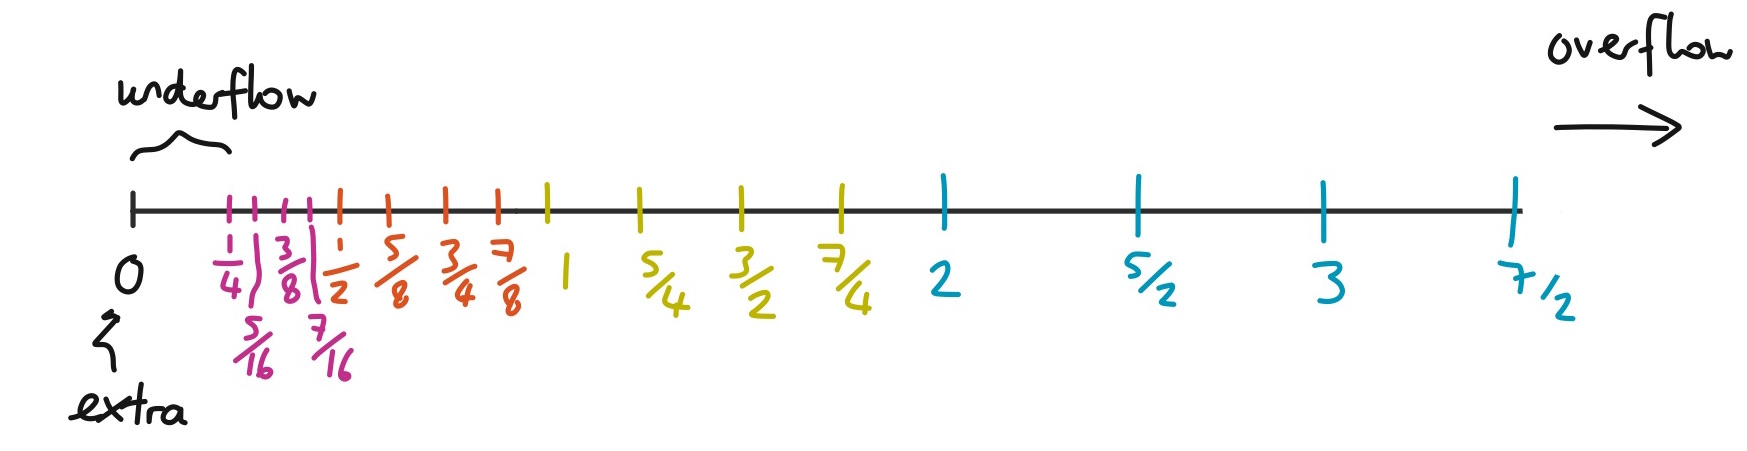
\includegraphics[width=0.9\linewidth,height=\textheight,keepaspectratio]{im/fp1.jpg}
\end{center}

\begin{tcolorbox}[enhanced jigsaw, bottomrule=.15mm, colbacktitle=quarto-callout-note-color!10!white, breakable, arc=.35mm, coltitle=black, colback=white, bottomtitle=1mm, opacityback=0, title=\textcolor{quarto-callout-note-color}{\faInfo}\hspace{0.5em}{Note}, titlerule=0mm, toptitle=1mm, opacitybacktitle=0.6, colframe=quarto-callout-note-color-frame, leftrule=.75mm, rightrule=.15mm, left=2mm, toprule=.15mm]

Notice that the spacing between numbers jumps by a factor \(\beta\) at
each power of \(\beta\). The largest possible number is
\((0.111)_22^2 = (\tfrac12 + \tfrac14 + \tfrac18)(4) = \tfrac72\). The
smallest non-zero number is
\((0.100)_22^{-1}=\tfrac12(\tfrac12) = \tfrac14\).

\end{tcolorbox}

Here \(\beta=2\), and there are 52 bits for the fraction, 11 for the
exponent, and 1 for the sign. The actual format used is \[
\pm (1.d_1\cdots d_{52})_22^{e-1023} = \pm (0.1d_1\cdots d_{52})_22^{e-1022}, \quad e = (e_1e_2\cdots e_{11})_2.
\] When \(\beta=2\), the first digit of a normalized number is always
\(1\), so doesn't need to be stored in memory. The \textbf{exponent
bias} of 1022 means that the actual exponents are in the range \(-1022\)
to \(1025\), since \(e\in[0,2047]\). Actually the exponents \(-1022\)
and \(1025\) are used to store \(\pm 0\) and \(\pm\infty\) respectively.

The smallest non-zero number in this system is
\((0.1)_22^{-1021} \approx 2.225\times 10^{-308}\), and the largest
number is \((0.1\cdots 1)_22^{1024} \approx 1.798\times 10^{308}\).

\begin{tcolorbox}[enhanced jigsaw, bottomrule=.15mm, colbacktitle=quarto-callout-note-color!10!white, breakable, arc=.35mm, coltitle=black, colback=white, bottomtitle=1mm, opacityback=0, title=\textcolor{quarto-callout-note-color}{\faInfo}\hspace{0.5em}{Note}, titlerule=0mm, toptitle=1mm, opacitybacktitle=0.6, colframe=quarto-callout-note-color-frame, leftrule=.75mm, rightrule=.15mm, left=2mm, toprule=.15mm]

IEEE stands for Institute of Electrical and Electronics Engineers.
Matlab uses the \href{https://en.wikipedia.org/wiki/IEEE_754}{IEEE 754}
standard for floating point arithmetic. The automatic 1 is sometimes
called the ``hidden bit''. The exponent bias avoids the need to store
the sign of the exponent.

\end{tcolorbox}

Numbers outside the finite set \(F\) cannot be represented exactly. If a
calculation falls below the lower non-zero limit (in absolute value), it
is called \textbf{underflow}, and usually set to 0. If it falls above
the upper limit, it is called \textbf{overflow}, and usually results in
a floating-point exception.

\begin{tcolorbox}[enhanced jigsaw, bottomrule=.15mm, colbacktitle=quarto-callout-note-color!10!white, breakable, arc=.35mm, coltitle=black, colback=white, bottomtitle=1mm, opacityback=0, title=\textcolor{quarto-callout-note-color}{\faInfo}\hspace{0.5em}{Note}, titlerule=0mm, toptitle=1mm, opacitybacktitle=0.6, colframe=quarto-callout-note-color-frame, leftrule=.75mm, rightrule=.15mm, left=2mm, toprule=.15mm]

\textbf{Ariane 5 rocket failure (1996):} The maiden flight ended in
failure. Only 40 seconds after initiation, at altitude 3700m, the
launcher veered off course and exploded. The cause was a software
exception during data conversion from a 64-bit float to a 16-bit
integer. The converted number was too large to be represented, causing
an exception.

\end{tcolorbox}

\begin{tcolorbox}[enhanced jigsaw, bottomrule=.15mm, colbacktitle=quarto-callout-note-color!10!white, breakable, arc=.35mm, coltitle=black, colback=white, bottomtitle=1mm, opacityback=0, title=\textcolor{quarto-callout-note-color}{\faInfo}\hspace{0.5em}{Note}, titlerule=0mm, toptitle=1mm, opacitybacktitle=0.6, colframe=quarto-callout-note-color-frame, leftrule=.75mm, rightrule=.15mm, left=2mm, toprule=.15mm]

In IEEE arithmetic, some numbers in the ``zero gap'' can be represented
using \(e=0\), since only two possible fraction values are needed for
\(\pm 0\). The other fraction values may be used with first (hidden) bit
0 to store a set of so-called \textbf{subnormal} numbers.

\end{tcolorbox}

The mapping from \(\mathbb{R}\) to \(F\) is called \textbf{rounding} and
denoted \(\mathrm{fl}(x)\). Usually it is simply the nearest number in
\(F\) to \(x\). If \(x\) lies exactly midway between two numbers in
\(F\), a method of breaking ties is required. The IEEE standard
specifies \emph{round to nearest even}---i.e., take the neighbour with
last digit 0 in the fraction.

\begin{tcolorbox}[enhanced jigsaw, bottomrule=.15mm, colbacktitle=quarto-callout-note-color!10!white, breakable, arc=.35mm, coltitle=black, colback=white, bottomtitle=1mm, opacityback=0, title=\textcolor{quarto-callout-note-color}{\faInfo}\hspace{0.5em}{Note}, titlerule=0mm, toptitle=1mm, opacitybacktitle=0.6, colframe=quarto-callout-note-color-frame, leftrule=.75mm, rightrule=.15mm, left=2mm, toprule=.15mm]

This avoids statistical bias or prolonged drift.

\end{tcolorbox}

\begin{center}
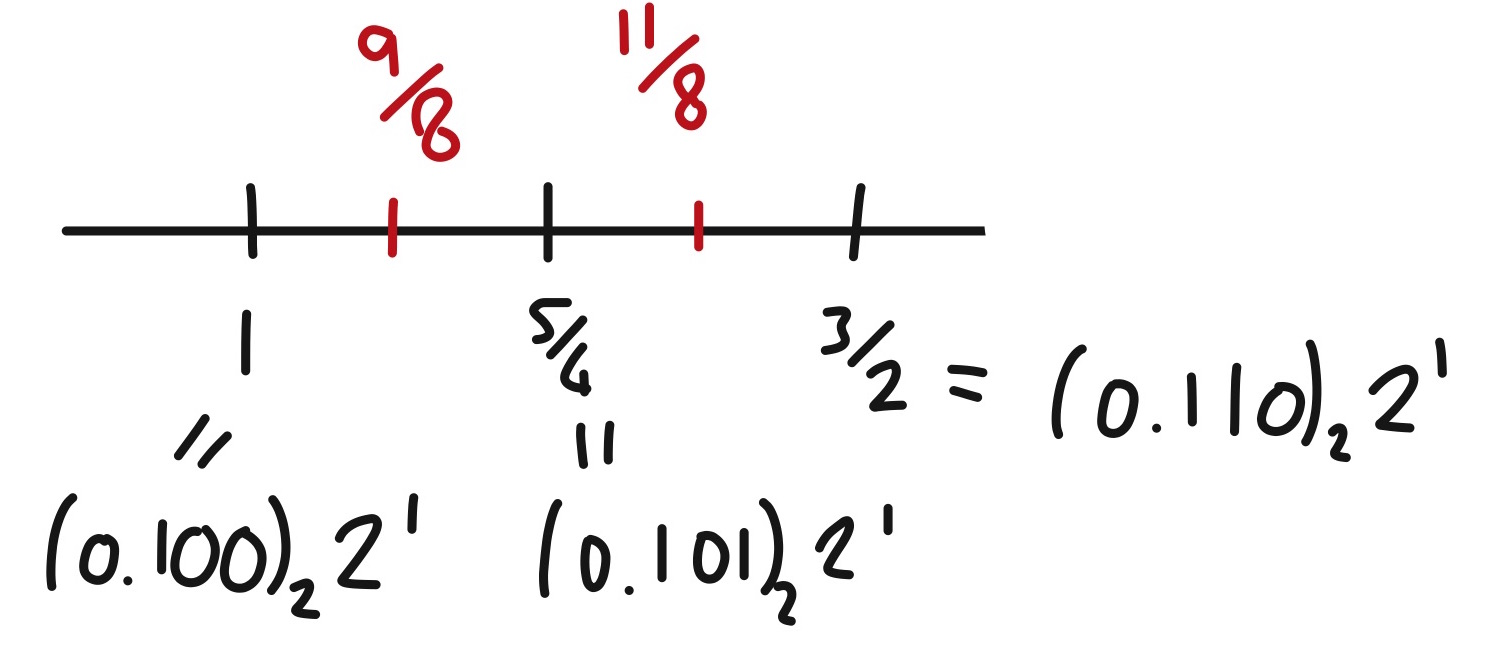
\includegraphics[width=0.7\linewidth,height=\textheight,keepaspectratio]{im/fp2.jpg}
\end{center}

\(\tfrac98 = (1.001)_2\) has neighbours \(1 = (0.100)_22^1\) and
\(\tfrac54 = (0.101)_22^1\), so is rounded down to \(1\).\\
\(\tfrac{11}{8} = (1.011)_2\) has neighbours \(\tfrac54 = (0.101)_22^1\)
and \(\tfrac32=(0.110)_22^1\), so is rounded up to \(\tfrac32\).

\begin{tcolorbox}[enhanced jigsaw, bottomrule=.15mm, colbacktitle=quarto-callout-note-color!10!white, breakable, arc=.35mm, coltitle=black, colback=white, bottomtitle=1mm, opacityback=0, title=\textcolor{quarto-callout-note-color}{\faInfo}\hspace{0.5em}{Note}, titlerule=0mm, toptitle=1mm, opacitybacktitle=0.6, colframe=quarto-callout-note-color-frame, leftrule=.75mm, rightrule=.15mm, left=2mm, toprule=.15mm]

\textbf{Vancouver stock exchange index:} In 1982, the index was
established at 1000. By November 1983, it had fallen to 520, even though
the exchange seemed to be doing well. Explanation: the index was rounded
\emph{down} to 3 digits at every recomputation. Since the errors were
always in the same direction, they added up to a large error over time.
Upon recalculation, the index doubled!

\end{tcolorbox}

\section{Significant figures}\label{significant-figures}

When doing calculations without a computer, we often use the terminology
of \textbf{significant figures}. To count the number of significant
figures in a number \(x\), start with the first non-zero digit from the
left, and count all the digits thereafter, including final zeros if they
are after the decimal point.

To round \(x\) to \(n\) s.f., replace \(x\) by the nearest number with
\(n\) s.f. An approximation \(\hat{x}\) of \(x\) is ``correct to \(n\)
s.f.'' if both \(\hat{x}\) and \(x\) round to the same number to \(n\)
s.f.

\section{Rounding error}\label{rounding-error}

There are two common ways of measuring the error of an approximation in
numerical analysis that we will use throughout the course:

\phantomsection\label{absolute-and-relative-errors}
\begin{fbxSimple}{definition}{Definition 1.1: }{Absolute and relative errors}
\phantomsection\label{absolute-and-relative-errors}
If \(x\) is the true value of a number and \(\hat{x}\) is an
approximation, we define the \textbf{absolute error} of this
approximation as the quantity \[
|\hat{x} - x|,
\] while the \textbf{relative error} of the approximation is given by \[
\frac{|\hat{x} - x|}{|x|},
\] assuming \(x \neq 0\).

\end{fbxSimple}

If \(|x|\) lies between the smallest non-zero number in \(F\) and the
largest number in \(F\), then \[
\mathrm{fl}(x) = x(1+\delta),
\] where the relative error incurred by rounding is \[
|\delta| = \frac{|\mathrm{fl}(x) - x|}{|x|}.
\]

\begin{tcolorbox}[enhanced jigsaw, bottomrule=.15mm, colbacktitle=quarto-callout-note-color!10!white, breakable, arc=.35mm, coltitle=black, colback=white, bottomtitle=1mm, opacityback=0, title=\textcolor{quarto-callout-note-color}{\faInfo}\hspace{0.5em}{Note}, titlerule=0mm, toptitle=1mm, opacitybacktitle=0.6, colframe=quarto-callout-note-color-frame, leftrule=.75mm, rightrule=.15mm, left=2mm, toprule=.15mm]

Relative errors are often more useful because they are scale invariant.
E.g., an error of 1 hour is irrelevant in estimating the age of a
lecture theatre, but catastrophic in timing your arrival at the lecture.

\end{tcolorbox}

Now \(x\) may be written as \(x=(0.d_1d_2\cdots)_\beta\beta^e\) for some
\(e\in[e_{\rm min},e_{\rm max}]\), but the fraction will not terminate
after \(m\) digits if \(x\notin F\). However, this fraction will differ
from that of \(\mathrm{fl}(x)\) by at most \(\tfrac12\beta^{-m}\), so \[
|\mathrm{fl}(x) - x| \leq \tfrac12\beta^{-m}\beta^e \quad \implies \quad |\delta| \leq \tfrac12\beta^{1-m}.
\] Here we used that the fractional part of \(|x|\) is at least
\((0.1)_\beta \equiv \beta^{-1}\). The number
\(\epsilon_{\rm M} = \tfrac12\beta^{1-m}\) is called the \textbf{machine
epsilon} (or \textbf{unit roundoff}), and is independent of \(x\). So
the relative rounding error satisfies \[
|\delta| \leq \epsilon_{\rm M}.
\]

\begin{tcolorbox}[enhanced jigsaw, bottomrule=.15mm, colbacktitle=quarto-callout-note-color!10!white, breakable, arc=.35mm, coltitle=black, colback=white, bottomtitle=1mm, opacityback=0, title=\textcolor{quarto-callout-note-color}{\faInfo}\hspace{0.5em}{Note}, titlerule=0mm, toptitle=1mm, opacitybacktitle=0.6, colframe=quarto-callout-note-color-frame, leftrule=.75mm, rightrule=.15mm, left=2mm, toprule=.15mm]

To check the machine epsilon value in Matlab you can just type `eps' in
the command line, which will return the value 2.2204e-16.

\end{tcolorbox}

\begin{tcolorbox}[enhanced jigsaw, bottomrule=.15mm, colbacktitle=quarto-callout-note-color!10!white, breakable, arc=.35mm, coltitle=black, colback=white, bottomtitle=1mm, opacityback=0, title=\textcolor{quarto-callout-note-color}{\faInfo}\hspace{0.5em}{Note}, titlerule=0mm, toptitle=1mm, opacitybacktitle=0.6, colframe=quarto-callout-note-color-frame, leftrule=.75mm, rightrule=.15mm, left=2mm, toprule=.15mm]

The name ``unit roundoff'' arises because \(\beta^{1-m}\) is the
distance between 1 and the next number in the system.

\end{tcolorbox}

When adding/subtracting/multiplying/dividing two numbers in \(F\), the
result will not be in \(F\) in general, so must be rounded.

Let us multiply \(x=\tfrac58\) and \(y=\tfrac78\). We have \[
xy = \tfrac{35}{64} = \tfrac12 + \tfrac1{32} + \tfrac1{64} = (0.100011)_2.
\] This has too many significant digits to represent in our system, so
the best we can do is round the result to
\(\mathrm{fl}(xy) = (0.100)_2 = \tfrac12\).

\begin{tcolorbox}[enhanced jigsaw, bottomrule=.15mm, colbacktitle=quarto-callout-note-color!10!white, breakable, arc=.35mm, coltitle=black, colback=white, bottomtitle=1mm, opacityback=0, title=\textcolor{quarto-callout-note-color}{\faInfo}\hspace{0.5em}{Note}, titlerule=0mm, toptitle=1mm, opacitybacktitle=0.6, colframe=quarto-callout-note-color-frame, leftrule=.75mm, rightrule=.15mm, left=2mm, toprule=.15mm]

Typically additional digits are used during the computation itself, as
in our example.

\end{tcolorbox}

For \({\circ} = +,-,\times, \div\), IEEE standard arithmetic requires
rounded exact operations, so that \[
\mathrm{fl}(x {\,\circ\,} y) = (x {\,\circ\,} y)(1+\delta), \quad |\delta|\leq\epsilon_{\rm M}.
\]

\section{Loss of significance}\label{loss-of-significance}

You might think that the above guarantees the accuracy of calculations
to within \(\epsilon_{\rm M}\), but this is true only if \(x\) and \(y\)
are themselves exact. In reality, we are probably starting from
\(\bar{x}=x(1+\delta_1)\) and \(\bar{y}=y(1 + \delta_2)\), with
\(|\delta_1|, |\delta_2| \leq \epsilon_{\rm M}\). In that case, there is
an error even before we round the result, since \[
\begin{aligned}
\bar{x} \pm \bar{y} &= x(1+ \delta_1) \pm y(1 + \delta_2)\\
&= (x\pm y)\left(1 + \frac{x\delta_1 \pm y\delta_2}{x\pm y}\right).
\end{aligned}
\] If the correct answer \(x\pm y\) is very small, then there can be an
arbitrarily large relative error in the result, compared to the errors
in the initial \(\bar{x}\) and \(\bar{y}\). In particular, this relative
error can be much larger than \(\epsilon_{\rm M}\). This is called
\textbf{loss of significance}, and is a major cause of errors in
floating-point calculations.

To 4 s.f., the roots are \[
x_1 = 28 + \sqrt{783} = 55.98, \quad x_2 = 28-\sqrt{783} = 0.01786.
\] However, working to 4 s.f. we would compute \(\sqrt{783} = 27.98\),
which would lead to the results \[
\bar{x}_1 = 55.98, \quad \bar{x}_2 = 0.02000.
\] The smaller root is not correct to 4 s.f., because of cancellation
error. One way around this is to note that
\(x^2 - 56x + 1 = (x-x_1)(x-x_2)\), and compute \(x_2\) from
\(x_2 = 1/x_1\), which gives the correct answer.

\begin{tcolorbox}[enhanced jigsaw, bottomrule=.15mm, colbacktitle=quarto-callout-note-color!10!white, breakable, arc=.35mm, coltitle=black, colback=white, bottomtitle=1mm, opacityback=0, title=\textcolor{quarto-callout-note-color}{\faInfo}\hspace{0.5em}{Note}, titlerule=0mm, toptitle=1mm, opacitybacktitle=0.6, colframe=quarto-callout-note-color-frame, leftrule=.75mm, rightrule=.15mm, left=2mm, toprule=.15mm]

Note that the error crept in when we rounded \(\sqrt{783}\) to
\(27.98\), because this removed digits that would otherwise have been
significant after the subtraction.

\end{tcolorbox}

Let us plot this function in the range
\(-5\times 10^{-8}\leq x \leq 5\times 10^{-8}\) -- even in IEEE double
precision arithmetic we find significant errors, as shown by the blue
curve:

\begin{center}
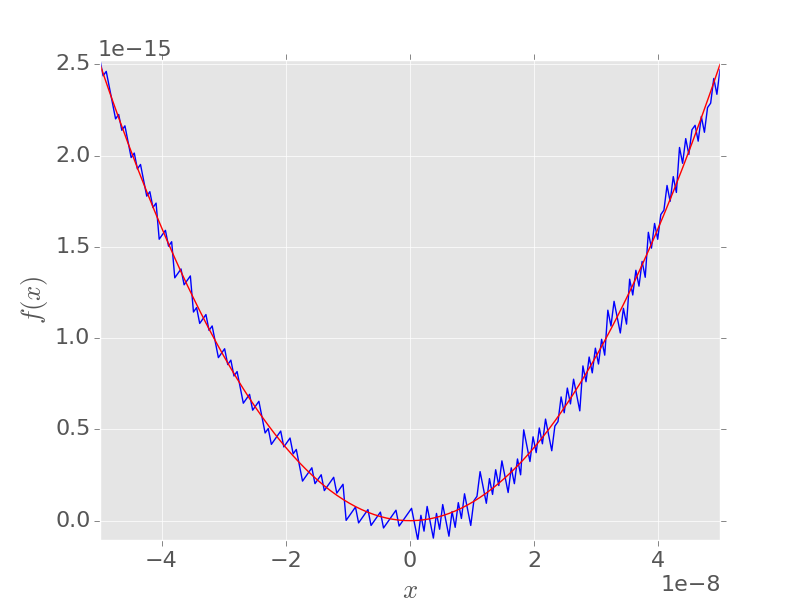
\includegraphics[width=0.7\linewidth,height=\textheight,keepaspectratio]{im/floating1.png}
\end{center}

The red curve shows the correct result approximated using the Taylor
series \[
\begin{aligned}
f(x) &= \left(1 + x + \frac{x^2}{2!} + \frac{x^3}{3!} + \ldots\right) - \left( 1 - \frac{x^2}{2!} + \frac{x^4}{4!} - \ldots\right) - x\\
&\approx x^2 + \frac{x^3}{6}.
\end{aligned}
\] This avoids subtraction of nearly equal numbers.

\begin{tcolorbox}[enhanced jigsaw, bottomrule=.15mm, colbacktitle=quarto-callout-note-color!10!white, breakable, arc=.35mm, coltitle=black, colback=white, bottomtitle=1mm, opacityback=0, title=\textcolor{quarto-callout-note-color}{\faInfo}\hspace{0.5em}{Note}, titlerule=0mm, toptitle=1mm, opacitybacktitle=0.6, colframe=quarto-callout-note-color-frame, leftrule=.75mm, rightrule=.15mm, left=2mm, toprule=.15mm]

We will look in more detail at polynomial approximations in the next
section.

\end{tcolorbox}

Note that floating-point arithmetic violates many of the usual rules of
real arithmetic, such as \((a+b)+c = a + (b+c)\).

\[
\begin{aligned}
\mathrm{fl}\big[(5.9 + 5.5) + 0.4\big] &= \mathrm{fl}\big[\mathrm{fl}(11.4) + 0.4\big] = \mathrm{fl}(11.0 + 0.4) = 11.0,\\
\mathrm{fl}\big[5.9 + (5.5 + 0.4)\big] &= \mathrm{fl}\big[5.9 + 5.9 \big] = \mathrm{fl}(11.8) = 12.0.
\end{aligned}
\]

In \(\mathbb{R}\), the average of two numbers always lies between the
numbers. But if we work to 3 decimal digits, \[
\mathrm{fl}\left(\frac{5.01 + 5.02}{2}\right) = \frac{\mathrm{fl}(10.03)}{2} = \frac{10.0}{2} = 5.0.
\]

The moral of the story is that sometimes care is needed to ensure that
we carry out a calculation accurately and as intended!

\section{Example: Weather Modelling}\label{example-weather-modelling}

A very simplistic description of an atmospheric fluid is given by the
\href{https://en.wikipedia.org/wiki/Lorenz_system}{Lorenz system of
differential equations}: \[
\begin{aligned}
\frac{dx}{dt} &= \sigma(y-x),\\
\frac{dy}{dt} &= x(\rho-z)-y,\\
\frac{dz}{dt} &= xy-\beta z,
\end{aligned}
\] where \(\sigma\), \(\rho\), and \(\beta\) are positive constants

We will describe how to solve such equations numerically in Chapter 5.
For now, let's look at a simulation of these equations computed by just
iterating a bunch of addition and multiplication steps:

\begin{center}
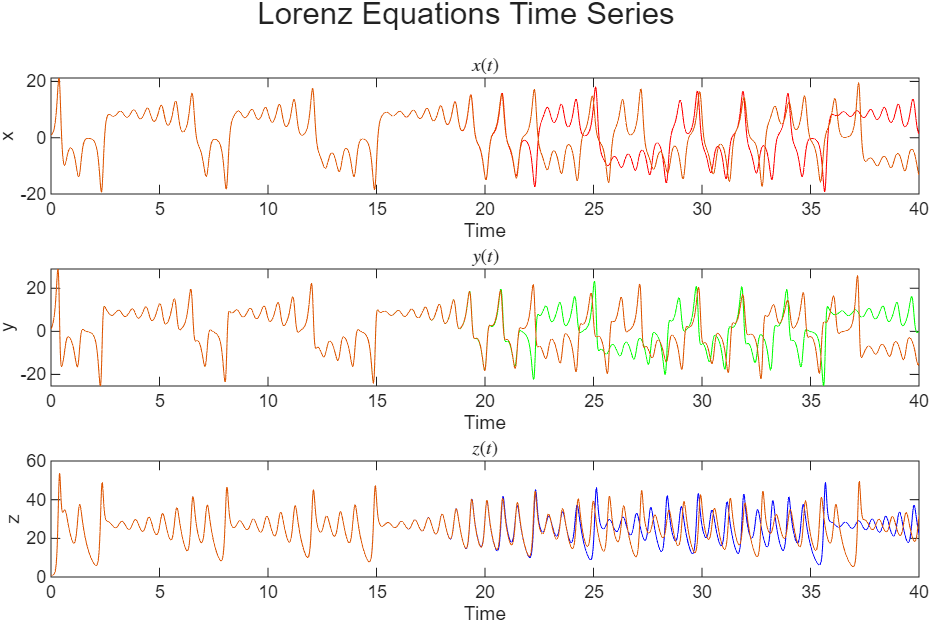
\includegraphics[width=0.7\linewidth,height=\textheight,keepaspectratio]{im/Lorenz.png}
\end{center}

Here we plot all three variables over a particular window of time
(loosely corresponding to something between minutes to hours, depending
on several details of the physics we are neglecting). For each variable,
we have ran two simulations with two different values of \(\beta\). One
simulation has \(\beta = 8/3 = 2.66666666666\dots\) and the other has
\(\beta = 8/3 + 10^{-10} = 2.66666666676\dots\). Nevertheless, you can
clearly see that this tiny difference in parameters (well below what is
experimentally measurable) has a huge impact on the solution. The reason
for this, and a key reason why weather is fundamentally hard to predict,
is the existence of
\href{https://en.wikipedia.org/wiki/Chaos_theory}{chaos} in many models
of physical phenomena. However truncation errors and floating point
errors also contribute to the discrepancies in this simulation.

The overall lesson of this Chapter so far is that small errors can exist
due to analytically-understood reasons such as the \emph{truncation
error} in a Taylor series approximation, or the \emph{floating point
error} in the numerical methods used. Such errors can not only impact
individual calculations, but they can accumulate and entirely change
outcomes of simulations, as we will see throughout the course.
Nevertheless, computational methods still underly an enormous range of
scientific fields, so understanding these sources of error (and how they
can become amplified) is a central theme of this course.

\section{Exact and symbolic
computing}\label{exact-and-symbolic-computing}

Symbolic computations require different data types from numerical ones;
in MATLAB we can use the
\href{https://uk.mathworks.com/help/symbolic/symbolic-computations-in-matlab.html}{Symbolic
Math Toolbox}. In the following chapters, we will compare symbolic and
numerical approaches to solving mathematical problems. One key
difference is that symbolic computations are exact, but much more
expensive to scale up to solve larger problems; for example, we will
tackle numerical problems involving matrices of size
\(10^4 \times 10^4\) or larger, which would not be possible to
successfully manipulate symbolically on a modern computer.

Symbolic computations are used to check or do laborious analytical work,
but also to rigorously prove mathematical Theorems which would be too
onerous to carry out by hand. FOr instance, while Lorenz equations above
were first noted to have strange dependencies on initial conditions, it
was only in 2002 that this was mathematically proved to be a chaotic
system. Among other tools, the proof relied on
\href{https://en.wikipedia.org/wiki/Interval_arithmetic}{interval
arithmetic}, which is a method to exactly operate on intervals defined
in terms of two rational numbers.

\section*{Knowledge checklist}\label{knowledge-checklist}
\addcontentsline{toc}{section}{Knowledge checklist}

\markright{Knowledge checklist}

\textbf{Key topics:}

\begin{enumerate}
\def\labelenumi{\arabic{enumi}.}
\item
  Integer and floating point representations of real numbers on
  computers.
\item
  Overflow, underflow and loss of significance.
\item
  Symbolic and numerical representations.
\end{enumerate}

\textbf{Key skills:}

\begin{itemize}
\item
  Understanding and distinguishing integer, fixed-point, and
  floating-point representations.
\item
  Analyzing the effects of rounding and machine epsilon in calculations.
\item
  Diagnosing and managing rounding errors, overflow, and underflow.
\end{itemize}

\bookmarksetup{startatroot}

\chapter{Continuous Functions}\label{continuous-functions}

The goal of this chapter is to explore and begin to answer the following
question:

\begin{quote}
\emph{How do we represent and manipulate continuous functions on a
computer?}
\end{quote}

\section{Interpolation}\label{interpolation}

\subsection{Polynomial Interpolation:
Motivation}\label{polynomial-interpolation-motivation}

The main idea of this section is to find a polynomial that approximates
a general function \(f\). But why polynomials? Polynomials have many
nice mathematical properties but from the perspective of function
approximation, the key one is the following: Any continuous function on
a compact interval can be approximated to arbitrary accuracy using a
polynomial (provided you are willing to go high enough degree).

\phantomsection\label{WAT}
\begin{fbxSimple}{theorem}{Theorem 2.1: }{Weierstrass Approximation Theorem (1885)}
\phantomsection\label{WAT}
For any \(f\in C([0,1])\) and any \(\epsilon > 0\), there exists a
polynomial \(p(x)\) such that \[
\max_{0\leq x\leq 1}\big|f(x) - p(x)\big| \leq \epsilon.
\]

\end{fbxSimple}

\begin{tcolorbox}[enhanced jigsaw, bottomrule=.15mm, colbacktitle=quarto-callout-note-color!10!white, breakable, arc=.35mm, coltitle=black, colback=white, bottomtitle=1mm, opacityback=0, title=\textcolor{quarto-callout-note-color}{\faInfo}\hspace{0.5em}{Note}, titlerule=0mm, toptitle=1mm, opacitybacktitle=0.6, colframe=quarto-callout-note-color-frame, leftrule=.75mm, rightrule=.15mm, left=2mm, toprule=.15mm]

This may be proved using an explicit sequence of polynomials, called
Bernstein polynomials.

\end{tcolorbox}

If \(f\) is a polynomial of degree \(n\), \[
f(x) = p_n(x) = a_0 + a_1x + \ldots + a_nx^n,
\] then we only need to store the \(n+1\) coefficients
\(a_0,\ldots,a_n\). Operations such as taking the derivative or
integrating \(f\) are also convenient. If \(f\) is not continuous, then
something other than a polynomial is required, since polynomials can't
handle asymptotic behaviour.

\begin{tcolorbox}[enhanced jigsaw, bottomrule=.15mm, colbacktitle=quarto-callout-note-color!10!white, breakable, arc=.35mm, coltitle=black, colback=white, bottomtitle=1mm, opacityback=0, title=\textcolor{quarto-callout-note-color}{\faInfo}\hspace{0.5em}{Note}, titlerule=0mm, toptitle=1mm, opacitybacktitle=0.6, colframe=quarto-callout-note-color-frame, leftrule=.75mm, rightrule=.15mm, left=2mm, toprule=.15mm]

To approximate functions like \(1/x\), there is a well-developed theory
of rational function interpolation, which is beyond the scope of this
course.

\end{tcolorbox}

In this chapter, we look for a suitable polynomial \(p_n\) by
\textbf{interpolation}---that is, requiring \(p_n(x_i) = f(x_i)\) at a
finite set of points \(x_i\), usually called \textbf{nodes}. Sometimes
we will also require the derivative(s) of \(p_n\) to match those of
\(f\). This type of function approximation where we want to match values
of the function that we know at particular points is very natural in
many applications. For example, weather forecasts involve numerically
solving huge systems of partial differential equations (PDEs), which
means actually solving them on a discrete grid of points. If we want
weather predictions between grid points, we must \textbf{interpolate}.
Figure~\ref{fig-MET} shows the spatial resolutions of a range of current
and past weather models produced by the UK Met Office.

\begin{figure}

\centering{

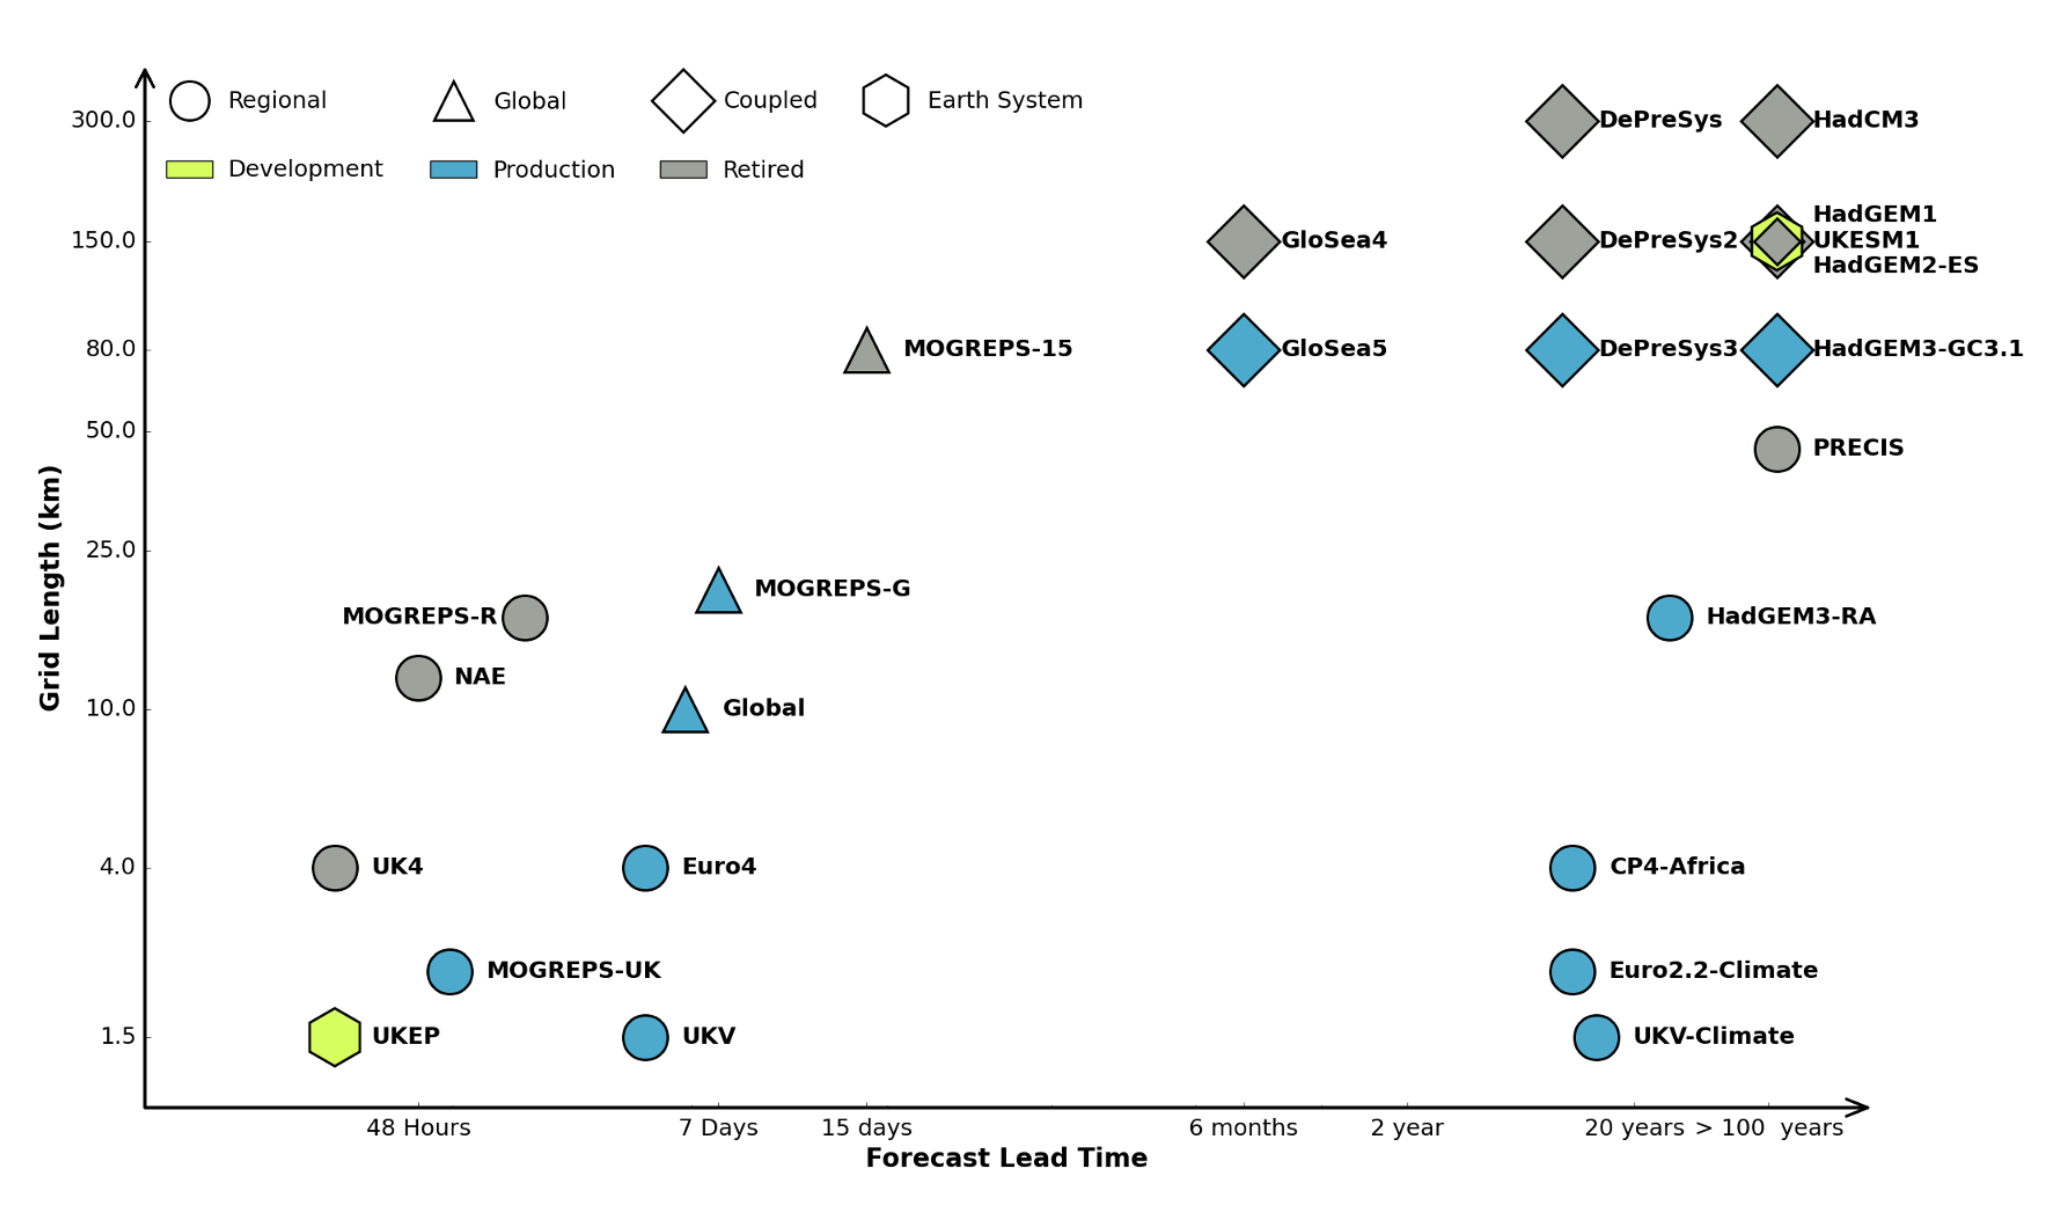
\includegraphics[width=0.85\linewidth,height=\textheight,keepaspectratio]{im/met_office.png}

}

\caption{\label{fig-MET}Chart showing a range of weather models produce
by the UK Met Office. Even the highest spatial resolution models have
more than 1.5km between grid point due to computational constraints.}

\end{figure}%

\subsection{Taylor series}\label{taylor-series}

A truncated Taylor series is (in some sense) the simplest interpolating
polynomial since it uses only a single node \(x_0\), although it does
require \(p_n\) to match both \(f\) and some of its derivatives.

We can approximate this using a Taylor series about the point \(x_0=0\),
which is \[
\sin(x) = x - \frac{x^3}{3!} + \frac{x^5}{5!} - \frac{x^7}{7!} + \ldots.
\] This comes from writing \[
f(x) = a_0 + a_1(x-x_0) + a_2(x-x_0)^2 + \ldots,
\] then differentiating term-by-term and matching values at \(x_0\):
\begin{align*}
f(x_0) &= a_0,\\
f'(x_0) &= a_1,\\
f''(x_0) &= 2a_2,\\
f'''(x_0) &= 3(2)a_3,\\
&\vdots\\
\implies f(x) &= f(x_0) + f'(x_0)(x-x_0) + \frac{f''(x_0)}{2!}(x-x_0)^2 + \frac{f'''(x_0)}{3!}(x-x_0)^3 + \ldots.
\end{align*} So \begin{align*}
\textrm{1 term} \;&\implies\; f(0.1) \approx 0.1,\\
\textrm{2 terms} \;&\implies\; f(0.1) \approx 0.1 - \frac{0.1^3}{6} = 0.099833\ldots,\\
\textrm{3 terms} \;&\implies\; f(0.1) \approx 0.1 - \frac{0.1^3}{6} + \frac{0.1^5}{120} = 0.09983341\ldots.\\
\end{align*} The next term will be
\(-0.1^7/7! \approx -10^{-7}/10^3 = -10^{-10}\), which won't change the
answer to 6 s.f.

\begin{tcolorbox}[enhanced jigsaw, bottomrule=.15mm, colbacktitle=quarto-callout-note-color!10!white, breakable, arc=.35mm, coltitle=black, colback=white, bottomtitle=1mm, opacityback=0, title=\textcolor{quarto-callout-note-color}{\faInfo}\hspace{0.5em}{Note}, titlerule=0mm, toptitle=1mm, opacitybacktitle=0.6, colframe=quarto-callout-note-color-frame, leftrule=.75mm, rightrule=.15mm, left=2mm, toprule=.15mm]

The exact answer is \(\sin(0.1)=0.09983341\dots\).

\end{tcolorbox}

Mathematically, we can write the remainder as follows.

\phantomsection\label{taylors-theorem}
\begin{fbxSimple}{theorem}{Theorem 2.2: }{Taylor’s Theorem}
\phantomsection\label{taylors-theorem}
Let \(f\) be \(n+1\) times differentiable on \((a,b)\), and let
\(f^{(n)}\) be continuous on \([a,b]\). If \(x,x_0\in[a,b]\) then there
exists \(\xi \in (a,b)\) such that \[
f(x) = \sum_{k=0}^n\frac{f^{(k)}(x_0)}{k!}(x-x_0)^k \; + \; \frac{f^{(n+1)}(\xi)}{(n+1)!}(x-x_0)^{n+1}.
\]

\end{fbxSimple}

The sum is called the \textbf{Taylor polynomial} of degree \(n\), and
the last term is called the \textbf{Lagrange form} of the remainder.
Note that the unknown number \(\xi\) depends on \(x\).

For \(f(x)=\sin(x)\), we found the Taylor polynomial
\(p_6(x) = x - x^3/3! + x^5/5!\), and \(f^{(7)}(x)=-\sin(x)\). So we
have \[
\big|f(x) - p_6(x)\big| = \left|\frac{f^{(7)}(\xi)}{7!}(x-x_0)^7\right|
\] for some \(\xi\) between \(x_0\) and \(x\). For \(x=0.1\), we have \[
\big|f(0.1) - p_6(0.1)\big| = \frac{1}{5040}(0.1)^7\big|f^{(7)}(\xi)\big| \quad \textrm{for some $\xi\in[0,0.1]$}.
\] Since \(\big|f^{(7)}(\xi)\big| = \big|\sin(\xi)\big| \leq 1\), we can
say, before calculating, that the error satisfies \[
\big|f(0.1) - p_6(0.1)\big| \leq 1.984\times 10^{-11}.
\]

\begin{tcolorbox}[enhanced jigsaw, bottomrule=.15mm, colbacktitle=quarto-callout-note-color!10!white, breakable, arc=.35mm, coltitle=black, colback=white, bottomtitle=1mm, opacityback=0, title=\textcolor{quarto-callout-note-color}{\faInfo}\hspace{0.5em}{Note}, titlerule=0mm, toptitle=1mm, opacitybacktitle=0.6, colframe=quarto-callout-note-color-frame, leftrule=.75mm, rightrule=.15mm, left=2mm, toprule=.15mm]

The actual error is \(1.983\times 10^{-11}\), so this is a tight
estimate.

\end{tcolorbox}

Since this error arises from approximating \(f\) with a truncated
series, rather than due to rounding, it is known as \textbf{truncation
error}. Note that it tends to be lower if you use more terms (larger
\(n\)), or if the function oscillates less (smaller \(f^{(n+1)}\) on the
interval \((x_0,x)\)).

Error estimates like the Lagrange remainder play an important role in
numerical analysis and computation, so it is important to understand
where it comes from. The number \(\xi\) will ultimately come from
Rolle's theorem, which is a special case of the mean value theorem from
first-year calculus:

\phantomsection\label{rolles-theorem}
\begin{fbxSimple}{theorem}{Theorem 2.3: }{Rolle’s Theorem}
\phantomsection\label{rolles-theorem}
If \(f\) is continuous on \([a,b]\) and differentiable on \((a,b)\),
with \(f(a)=f(b)=0\), then there exists \(\xi\in(a,b)\) with
\(f'(\xi)=0\).

\end{fbxSimple}

\begin{tcolorbox}[enhanced jigsaw, bottomrule=.15mm, colbacktitle=quarto-callout-note-color!10!white, breakable, arc=.35mm, coltitle=black, colback=white, bottomtitle=1mm, opacityback=0, title=\textcolor{quarto-callout-note-color}{\faInfo}\hspace{0.5em}{Note}, titlerule=0mm, toptitle=1mm, opacitybacktitle=0.6, colframe=quarto-callout-note-color-frame, leftrule=.75mm, rightrule=.15mm, left=2mm, toprule=.15mm]

Note that Rolle's Theorem does not tell us what the value of \(\xi\)
might actually be, so in practice we must take some kind of worst case
estimate to get an error bound, e.g.~calculate the max value of
\(f'(\xi)\) over the range of possible \(\xi\) values.

\end{tcolorbox}

\subsection{Polynomial Interpolation}\label{polynomial-interpolation}

The classical problem of \textbf{polynomial interpolation} is to find a
polynomial \[
p_n(x) = a_0 + a_1x + \ldots + a_n x^n = \sum_{k=0}^n a_k x^k
\] that interpolates our function \(f\) at a finite set of nodes
\(\{x_0, x_1, \ldots, x_m\}\). In other words, \(p_n(x_i)=f(x_i)\) at
each of the nodes \(x_i\). Since the polynomial has \(n+1\) unknown
coefficients, we expect to need \(n+1\) distinct nodes, so let us assume
that \(m=n\).

Here we have two nodes \(x_0\), \(x_1\), and seek a polynomial
\(p_1(x) = a_0 + a_1x\). Then the interpolation conditions require that
\[
\begin{cases}
p_1(x_0) = a_0 + a_1x_0 = f(x_0)\\
p_1(x_1) = a_0 + a_1x_1 = f(x_1)
\end{cases}
\implies\quad
p_1(x) = \frac{x_1f(x_0) - x_0f(x_1)}{x_1 - x_0} + \frac{f(x_1) - f(x_0)}{x_1 - x_0}x.
\]

For general \(n\), the interpolation conditions require \[
\begin{matrix}
a_0 &+ a_1x_0 &+ a_2x_0^2 &+ \ldots &+ a_nx_0^n &= f(x_0),\\
a_0 &+ a_1x_1 &+ a_2x_1^2 &+ \ldots &+ a_nx_1^n &= f(x_1),\\
\vdots  & \vdots  & \vdots     &        &\vdots      & \vdots\\
a_0 &+ a_1x_n &+ a_2x_n^2 &+ \ldots &+ a_nx_n^n &= f(x_n),
\end{matrix}
\] so we have to solve \[
\begin{pmatrix}
1 & x_0 & x_0^2 & \cdots & x_0^n\\
1 & x_1 & x_1^2 & \cdots & x_1^n\\
\vdots & \vdots &\vdots& & \vdots\\
1 & x_n & x_n^2 & \cdots & x_n^n\\
\end{pmatrix}
\begin{pmatrix}
a_0\\ a_1\\ \vdots\\ a_n
\end{pmatrix}
=
\begin{pmatrix}
f(x_0)\\ f(x_1)\\ \vdots\\ f(x_n)
\end{pmatrix}.
\] This is called a \textbf{Vandermonde matrix}. The determinant of this
matrix is \[
\det(A) = \prod_{0\leq i < j\leq n} (x_j - x_i),
\] which is non-zero provided the nodes are all distinct. This
establishes an important result, where \(\mathcal{P}_n\) denotes the
space of all real polynomials of degree \(\leq n\).

\phantomsection\label{existenceuniqueness}
\begin{fbxSimple}{theorem}{Theorem 2.4: }{Existence/uniqueness}
\phantomsection\label{existenceuniqueness}
Given \(n+1\) distinct nodes \(x_0, x_1, \ldots, x_n\), there is a
unique polynomial \(p_n\in\mathcal{P}_n\) that interpolates \(f(x)\) at
these nodes.

\end{fbxSimple}

We may also prove uniqueness by the following elegant argument.

\textbf{Proof (Uniqueness part of Existence/Uniqueness Theorem):}\\
Suppose that in addition to \(p_n\) there is another interpolating
polynomial \(q_n\in\mathcal{P}_n\). Then the difference
\(r_n := p_n - q_n\) is also a polynomial with degree \(\leq n\). But we
have \[
r_n(x_i) = p_n(x_i) - q_n(x_i) = f(x_i)-f(x_i)=0 \quad \textrm{for $i=0,\ldots,n$},
\] so \(r_n(x)\) has \(n+1\) roots. From the Fundamental Theorem of
Algebra, this is possible only if \(r_n(x)\equiv 0\), which implies that
\(q_n=p_n\).

\begin{tcolorbox}[enhanced jigsaw, bottomrule=.15mm, colbacktitle=quarto-callout-note-color!10!white, breakable, arc=.35mm, coltitle=black, colback=white, bottomtitle=1mm, opacityback=0, title=\textcolor{quarto-callout-note-color}{\faInfo}\hspace{0.5em}{Note}, titlerule=0mm, toptitle=1mm, opacitybacktitle=0.6, colframe=quarto-callout-note-color-frame, leftrule=.75mm, rightrule=.15mm, left=2mm, toprule=.15mm]

Note that the unique polynomial through \(n+1\) points may have degree
\(< n\). This happens when \(a_0=0\) in the solution to the Vandermonde
system above.

\end{tcolorbox}

\phantomsection\label{interpolate-fxcosx-with-p_2inmathcalp_2-at-the-nodes-0-tfracpi2-pi.}
\begin{fbxSimple}{eg}{Example 2.1: }{Interpolate \(f(x)=\cos(x)\) with \(p_2\in\mathcal{P}_2\) at the nodes \(\{0, \tfrac{\pi}{2}, \pi\}\).}
\phantomsection\label{interpolate-fxcosx-with-p_2inmathcalp_2-at-the-nodes-0-tfracpi2-pi.}
We have \(x_0=0\), \(x_1=\tfrac{\pi}{2}\), \(x_2=\pi\), so \(f(x_0)=1\),
\(f(x_1)=0\), \(f(x_2)=-1\). Clearly the unique interpolant is a
straight line \(p_2(x) = 1 - \tfrac2\pi x\).

If we took the nodes \(\{0,2\pi,4\pi\}\), we would get a constant
function \(p_2(x)=1\).

\begin{center}
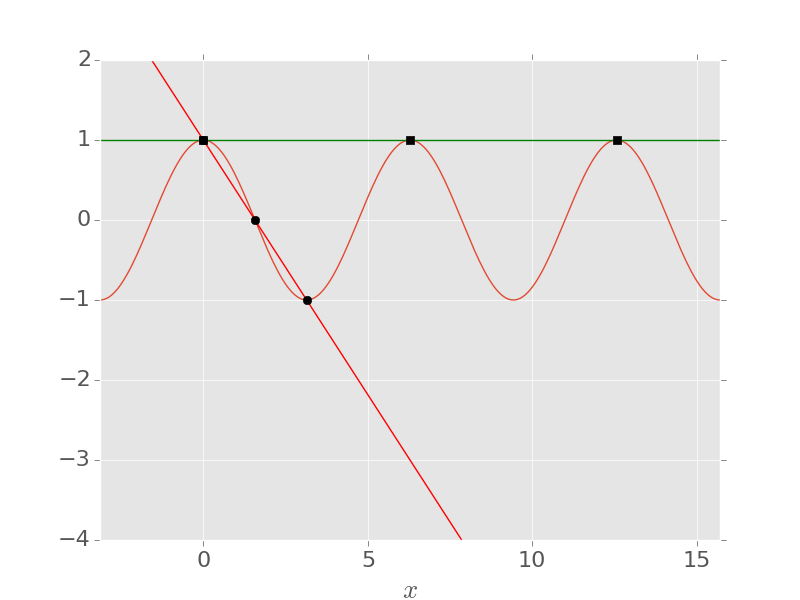
\includegraphics[width=0.7\linewidth,height=\textheight,keepaspectratio]{im/linear_interp.png}
\end{center}

\end{fbxSimple}

One way to compute the interpolating polynomial would be to solve the
Vandermonde system above, e.g.~by Gaussian elimination. However, this is
not recommended. In practice, we choose a different basis for \(p_n\);
there are two common and effective choices due to Lagrange and Newton.

\begin{tcolorbox}[enhanced jigsaw, bottomrule=.15mm, colbacktitle=quarto-callout-note-color!10!white, breakable, arc=.35mm, coltitle=black, colback=white, bottomtitle=1mm, opacityback=0, title=\textcolor{quarto-callout-note-color}{\faInfo}\hspace{0.5em}{Note}, titlerule=0mm, toptitle=1mm, opacitybacktitle=0.6, colframe=quarto-callout-note-color-frame, leftrule=.75mm, rightrule=.15mm, left=2mm, toprule=.15mm]

The Vandermonde matrix arises when we write \(p_n\) in the
\textbf{natural basis} \(\{1,x,x^2,\ldots\}\), but we could also choose
to work in some other basis\ldots{}

\end{tcolorbox}

\subsection{Lagrange Polynomials}\label{sec-polylag}

This uses a special basis of polynomials \(\{\ell_k\}\) in which the
interpolation equations reduce to the identity matrix. In other words,
the coefficients in this basis are just the function values, \[
p_n(x) = \sum_{k=0}^n f(x_k)\ell_k(x).
\]

\phantomsection\label{eg-2.2}
\begin{fbxSimple}{eg}{Example 2.2: }{Linear interpolation again.}
\phantomsection\label{eg-2.2}
We can re-write our linear interpolant to separate out the function
values: \[
p_1(x) = \underbrace{\frac{x - x_1}{x_0 - x_1}}_{\ell_0(x)}f(x_0) + \underbrace{\frac{x-x_0}{x_1-x_0}}_{\ell_1(x)}f(x_1).
\] Then \(\ell_0\) and \(\ell_1\) form the necessary basis. In
particular, they have the property that \[
\ell_0(x_i) = \begin{cases}
1 & \textrm{if $i=0$},\\
0 & \textrm{if $i=1$},
\end{cases}
\qquad
\ell_1(x_i) = \begin{cases}
0 & \textrm{if $i=0$},\\
1 & \textrm{if $i=1$},
\end{cases}
\]

\end{fbxSimple}

For general \(n\), the \(n+1\) \textbf{Lagrange polynomials} are defined
as a product \[
\ell_k(x) = \prod_{\substack{j=0\\j\neq k}}^n\frac{x - x_j}{x_k - x_j}.
\] By construction, they have the property that \[
\ell_k(x_i) = \begin{cases}
1 & \textrm{if $i=k$},\\
0 & \textrm{otherwise}.
\end{cases}
\] From this, it follows that the interpolating polynomial may be
written as above.

\begin{tcolorbox}[enhanced jigsaw, bottomrule=.15mm, colbacktitle=quarto-callout-note-color!10!white, breakable, arc=.35mm, coltitle=black, colback=white, bottomtitle=1mm, opacityback=0, title=\textcolor{quarto-callout-note-color}{\faInfo}\hspace{0.5em}{Note}, titlerule=0mm, toptitle=1mm, opacitybacktitle=0.6, colframe=quarto-callout-note-color-frame, leftrule=.75mm, rightrule=.15mm, left=2mm, toprule=.15mm]

By the Existence/Uniqueness Theorem, the Lagrange polynomials are the
\emph{unique} polynomials with this property.

\end{tcolorbox}

\phantomsection\label{compute-the-quadratic-interpolating-polynomial-to-fxcosx-with-nodes--tfracpi4-0-tfracpi4-using-lagrange-polynomials.}
\begin{fbxSimple}{eg}{Example 2.3: }{Compute the quadratic interpolating polynomial to \(f(x)=\cos(x)\) with nodes \(\{-\tfrac\pi4, 0, \tfrac\pi4\}\) using Lagrange polynomials.}
\phantomsection\label{compute-the-quadratic-interpolating-polynomial-to-fxcosx-with-nodes--tfracpi4-0-tfracpi4-using-lagrange-polynomials.}
The Lagrange polynomials of degree 2 for these nodes are \[
\begin{aligned}
\ell_0(x) &= \frac{(x-x_1)(x-x_2)}{(x_0-x_1)(x_0-x_2)} = \frac{x(x-\tfrac\pi4)}{\tfrac\pi4\cdot\tfrac\pi2},\\
\ell_1(x) &= \frac{(x-x_0)(x-x_2)}{(x_1-x_0)(x_1-x_2)} = \frac{(x+\tfrac\pi4)(x-\tfrac\pi4)}{-\tfrac\pi4\cdot\tfrac\pi4},\\
\ell_2(x) &= \frac{(x-x_0)(x-x_1)}{(x_2-x_0)(x_2-x_1)}\\ 
&= \frac{x(x+\tfrac\pi4)}{\tfrac\pi2\cdot\tfrac\pi4}.
\end{aligned}
\] So the interpolating polynomial is \[
\begin{aligned}
p_2(x) &= f(x_0)\ell_0(x) + f(x_1)\ell_1(x) + f(x_2)\ell_2(x)\\
&= \tfrac{1}{\sqrt{2}}\tfrac8{\pi^2}x(x-\tfrac\pi4) - \tfrac{16}{\pi^2}(x+\tfrac\pi4)(x-\tfrac\pi4) +\tfrac{1}{\sqrt{2}}\tfrac8{\pi^2}x(x+\tfrac\pi4) = \tfrac{16}{\pi^2}\big(\tfrac{1}{\sqrt{2}} - 1\big)x^2 + 1.
\end{aligned}
\] The Lagrange polynomials and the resulting interpolant are shown
below:

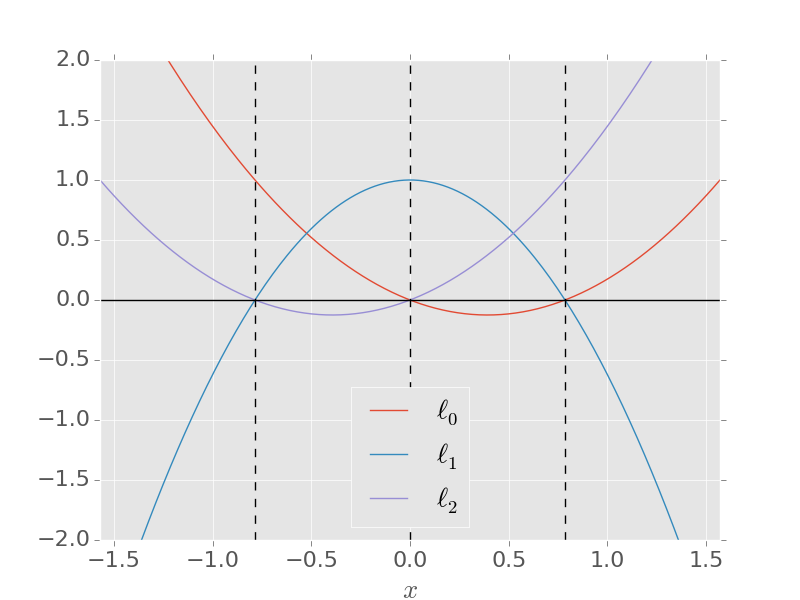
\includegraphics[width=0.45\linewidth,height=\textheight,keepaspectratio]{im/lagrange_polys.png}
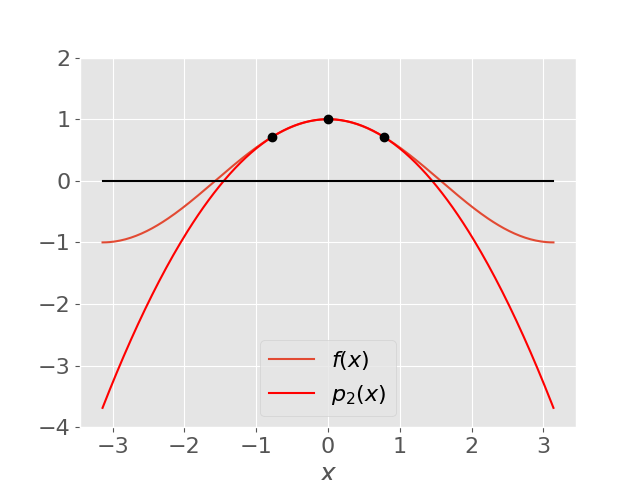
\includegraphics[width=0.45\linewidth,height=\textheight,keepaspectratio]{im/lagrange.png}

\end{fbxSimple}

\begin{tcolorbox}[enhanced jigsaw, bottomrule=.15mm, colbacktitle=quarto-callout-note-color!10!white, breakable, arc=.35mm, coltitle=black, colback=white, bottomtitle=1mm, opacityback=0, title=\textcolor{quarto-callout-note-color}{\faInfo}\hspace{0.5em}{Note}, titlerule=0mm, toptitle=1mm, opacitybacktitle=0.6, colframe=quarto-callout-note-color-frame, leftrule=.75mm, rightrule=.15mm, left=2mm, toprule=.15mm]

Lagrange polynomials were actually discovered by Edward Waring in 1776
and rediscovered by Euler in 1783, before they were published by
Lagrange himself in 1795; a classic example of Stigler's law of eponymy!

\end{tcolorbox}

The Lagrange form of the interpolating polynomial is easy to write down,
but expensive to evaluate since all of the \(\ell_k\) must be computed.
Moreover, changing any of the nodes means that the \(\ell_k\) must all
be recomputed from scratch, and similarly for adding a new node (moving
to higher degree).

\subsection{Newton/Divided-Difference
Polynomials}\label{newtondivided-difference-polynomials}

It would be easy to increase the degree of \(p_n\) if \[
p_{n+1}(x) = p_{n}(x) + g_{n+1}(x), \quad \textrm{where $g_{n+1}\in{\cal P}_{n+1}$}.
\] From the interpolation conditions, we know that \[
g_{n+1}(x_i) = p_{n+1}(x_i) - p_{n}(x_i) = f(x_i)-f(x_i)=0 \quad \textrm{for $i=0,\ldots,n$},
\] so \[
g_{n+1}(x) = a_{n+1}(x-x_0)\cdots(x-x_{n}).
\] The coefficient \(a_{n+1}\) is determined by the remaining
interpolation condition at \(x_{n+1}\), so \[
p_n(x_{n+1}) + g_{n+1}(x_{n+1}) = f(x_{n+1}) \quad \implies \quad a_{n+1} = \frac{f(x_{n+1}) - p_{n}(x_{n+1})}{(x_{n+1}-x_0)\cdots(x_{n+1}-x_{n})}.
\]

The polynomial \((x-x_0)(x-x_1)\cdots(x-x_{n})\) is called a
\textbf{Newton polynomial}. These form a new basis \[
n_0(x)=1, \qquad n_k(x) = \prod_{j=0}^{k-1}(x-x_j) \quad \textrm{for $k>0$}.
\]

The \textbf{Newton form} of the interpolating polynomial is then \[
p_n(x) = \sum_{k=0}^n a_kn_k(x), \qquad a_0 = f(x_0),\qquad a_k = \frac{f(x_k) - p_{k-1}(x_k)}{(x_k-x_0)\cdots(x_k-x_{k-1})} \textrm{ for $k>0$}.
\] Notice that \(a_k\) depends only on \(x_0,\ldots x_k\), so we can
construct first \(a_0\), then \(a_1\), etc.

It turns out that the \(a_k\) are easy to compute, but it will take a
little work to derive the method. We define the \textbf{divided
difference} \(f[x_0,x_1,\ldots,x_k]\) to be the coefficient of \(x^k\)
in the polynomial interpolating \(f\) at nodes \(x_0,\ldots,x_k\). It
follows that \[
f[x_0,x_1,\ldots,x_k] = a_k,
\] where \(a_k\) is the coefficient in the Newton form above.

\phantomsection\label{eg-2.4}
\begin{fbxSimple}{eg}{Example 2.4: }{Compute the Newton interpolating polynomial at two nodes.}
\phantomsection\label{eg-2.4}
\[
\begin{aligned}
f[x_0] &= a_0 = f(x_0),\\
f[x_0,x_1] &= a_1 = \frac{f(x_1) - p_0(x_1)}{x_1 - x_0} = \frac{f(x_1)-a_0}{x_1 - x_0} = \frac{f[x_1]-f[x_0]}{x_1 - x_0}.
\end{aligned}
\] So the \textbf{first-order} divided difference \(f[x_0,x_1]\) is
obtained from the \textbf{zeroth-order} differences \(f[x_0]\),
\(f[x_1]\) by subtracting and dividing, hence the name ``divided
difference''.

\end{fbxSimple}

\phantomsection\label{eg-2.5}
\begin{fbxSimple}{eg}{Example 2.5: }{Compute the Newton interpolating polynomial at three nodes.}
\phantomsection\label{eg-2.5}
Continuing from the previous example, we find \[
\begin{aligned}
f[x_0,x_1,x_2] &= a_2 = \frac{f(x_2) - p_1(x_2)}{(x_2 - x_0)(x_2-x_1)} = \frac{f(x_2) - a_0 - a_1(x_2-x_0)}{(x_2 - x_0)(x_2-x_1)}\\
& = \ldots = \frac{1}{x_2-x_0}\left(\frac{f[x_2]-f[x_1]}{x_2-x_1} - \frac{f[x_1]-f[x_0]}{x_1-x_0}\right)\\
&= \frac{f[x_1,x_2]-f[x_0,x_1]}{x_2-x_0}.
\end{aligned}
\] So again, we subtract and divide.

\end{fbxSimple}

In general, we have the following.

\phantomsection\label{theorem-2.5}
\begin{fbxSimple}{theorem}{Theorem 2.5}{}
\phantomsection\label{theorem-2.5}
For \(k>0\), the divided differences satisfy \[
f[x_i,x_{i+1},\ldots,x_{i+k}] = \frac{f[x_{i+1},\ldots,x_{i+k}] - f[x_i,\ldots,x_{i+k-1}]}{x_{i+k} - x_i}.
\]

\end{fbxSimple}

\textbf{Proof:}\\
Without loss of generality, we relabel the nodes so that \(i=0\). So we
want to prove that \[
f[x_0,x_1,\ldots,x_{k}] = \frac{f[x_1,\ldots,x_{k}] - f[x_0,\ldots,x_{k-1}]}{x_{k} - x_0}.
\] The trick is to write the interpolant with nodes \(x_0, \ldots, x_k\)
in the form \[
p_k(x) = \frac{(x_k-x)q_{k-1}(x) + (x-x_0)\tilde{q}_{k-1}(x)}{x_k-x_0},
\] where \(q_{k-1}\in{\cal P}_{k-1}\) interpolates \(f\) at the subset
of nodes \(x_0, x_1, \ldots, x_{k-1}\) and
\(\tilde{q}_{k-1}\in{\cal P}_{k-1}\) interpolates \(f\) at the subset
\(x_1, x_2,\ldots,x_k\). If this holds, then matching the coefficient of
\(x^k\) on each side will give the divided difference formula, since,
e.g., the leading coefficient of \(q_{k-1}\) is
\(f[x_0,\ldots,x_{k-1}]\). To see that \(p_k\) may really be written
this way, note that \[
\begin{aligned}
p_k(x_0) &= q_{k-1}(x_0) = f(x_0),\\
p_k(x_k) &= \tilde{q}_{k-1}(x_k) = f(x_k),\\
p_k(x_i) &= \frac{(x_k-x_i)q_{k-1}(x_i) + (x_i-x_0)\tilde{q}_{k-1}(x_i)}{x_k - x_0} = f(x_i) \quad \textrm{for $i=1,\ldots,k-1$}.
\end{aligned}
\] Since \(p_k\) agrees with \(f\) at the \(k+1\) nodes, it is the
unique interpolant in \({\cal P}_k\).

Theorem above gives us our convenient method, which is to construct a
\textbf{divided-difference table}.

\phantomsection\label{construct-the-newton-polynomial-at-the-nodes--1012-and-with-corresponding-function-values-51111}
\begin{fbxSimple}{eg}{Example 2.6: }{Construct the Newton polynomial at the nodes \(\{-1,0,1,2\}\) and with corresponding function values \(\{5,1,1,11\}\)}
\phantomsection\label{construct-the-newton-polynomial-at-the-nodes--1012-and-with-corresponding-function-values-51111}
We construct a divided-difference table as follows. \[
\begin{matrix}
&x_0=-1 \quad &f[x_0]=5 & & &\\
& & &f[x_0,x_1]=-4 & &\\
&x_1=0 \quad &f[x_1]=1 & &f[x_0,x_1,x_2]=2 &\\
& & &f[x_1,x_2]=0 & &f[x_0,x_1,x_2,x_3]=1\\
&x_2=1 \quad &f[x_2]=1 & &f[x_1,x_2,x_3]=5 &\\
& & &f[x_2,x_3]=10 & &\\
&x_3=2 \quad &f[x_3]=11 & & &\\
\end{matrix}
\] The coefficients of the \(p_3\) lie at the top of each column, so \[
\begin{aligned}
p_3(x) &= f[x_0] + f[x_0,x_1](x-x_0) + f[x_0,x_1,x_2](x-x_0)(x-x_1)\\
& + f[x_0,x_1,x_2,x_3](x-x_0)(x-x_1)(x-x_2)\\
&=5 - 4(x+1) + 2x(x+1) + x(x+1)(x-1).
\end{aligned}
\] Now suppose we add the extra nodes \(\{-2,3\}\) with data
\(\{5,35\}\). All we need to do to compute \(p_5\) is add two rows to
the bottom of the table --- there is no need to recalculate the rest.
This gives \[
\begin{matrix}
&-1  &5 & & & & &\\
& & &-4 & & & &\\
&0  &1 & &2 & & &\\
& & &0 & &1 & &\\
&1  &1 & &5 & &\textcolor{red}{-\tfrac1{12}} &\\
& & &10 & &\textcolor{red}{\tfrac{13}{12}} & &\textcolor{red}{0}\\
&2 &11 & &\textcolor{red}{\tfrac{17}{6}} & &\textcolor{red}{-\tfrac1{12}}\\
& & &\textcolor{red}{\tfrac{3}{2}} & &\textcolor{red}{\tfrac{5}{6}} & &\\
&\textcolor{red}{-2} &\textcolor{red}{5} & &\textcolor{red}{\tfrac92} & &&\\
& & &\textcolor{red}{6} & & & &\\
&\textcolor{red}{3}  &\textcolor{red}{35} & & & & &\\
\end{matrix}
\] The new interpolating polynomial is \[
p_5(x) = p_3(x) - \tfrac{1}{12}x(x+1)(x-1)(x-2).
\]

\end{fbxSimple}

\begin{tcolorbox}[enhanced jigsaw, bottomrule=.15mm, colbacktitle=quarto-callout-note-color!10!white, breakable, arc=.35mm, coltitle=black, colback=white, bottomtitle=1mm, opacityback=0, title=\textcolor{quarto-callout-note-color}{\faInfo}\hspace{0.5em}{Note}, titlerule=0mm, toptitle=1mm, opacitybacktitle=0.6, colframe=quarto-callout-note-color-frame, leftrule=.75mm, rightrule=.15mm, left=2mm, toprule=.15mm]

Notice that the \(x^5\) coefficient vanishes for these particular data,
meaning that they are consistent with \(f\in{\cal P}_4\).

\end{tcolorbox}

\begin{tcolorbox}[enhanced jigsaw, bottomrule=.15mm, colbacktitle=quarto-callout-note-color!10!white, breakable, arc=.35mm, coltitle=black, colback=white, bottomtitle=1mm, opacityback=0, title=\textcolor{quarto-callout-note-color}{\faInfo}\hspace{0.5em}{Note}, titlerule=0mm, toptitle=1mm, opacitybacktitle=0.6, colframe=quarto-callout-note-color-frame, leftrule=.75mm, rightrule=.15mm, left=2mm, toprule=.15mm]

Note that the value of \(f[x_0,x_1,\ldots,x_k]\) is independent of the
order of the nodes in the table. This follows from the uniqueness of
\(p_k\).

\end{tcolorbox}

Divided differences are actually approximations for \emph{derivatives}
of \(f\). In the limit that the nodes all coincide, the Newton form of
\(p_n(x)\) becomes the Taylor polynomial.

\subsection{Interpolation Error}\label{interpolation-error}

The goal here is to estimate the error \(|f(x)-p_n(x)|\) when we
approximate a function \(f\) by a polynomial interpolant \(p_n\).
Clearly this will depend on \(x\).

\phantomsection\label{quadratic-interpolant-for-fxcosx-with--tfracpi40tfracpi4.}
\begin{fbxSimple}{eg}{Example 2.7: }{Quadratic interpolant for \(f(x)=\cos(x)\) with \(\{-\tfrac\pi4,0,\tfrac\pi4\}\).}
\phantomsection\label{quadratic-interpolant-for-fxcosx-with--tfracpi40tfracpi4.}
From Section~\ref{sec-polylag}, we have
\(p_2(x) = \tfrac{16}{\pi^2}\left(\tfrac{1}{\sqrt{2}}-1\right)x^2 + 1\),
so the error is \[
|f(x) - p_2(x)| = \left|\cos(x) -  \tfrac{16}{\pi^2}\left(\tfrac{1}{\sqrt{2}}-1\right)x^2 - 1\right|.
\] This is shown below:

\begin{center}
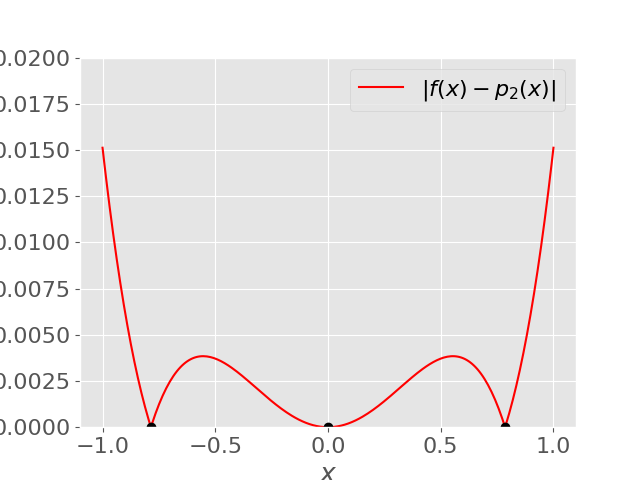
\includegraphics[width=0.7\linewidth,height=\textheight,keepaspectratio]{im/lagrange_error.png}
\end{center}

Clearly the error vanishes at the nodes themselves, but note that it
generally does better near the middle of the set of nodes --- this is
quite typical behaviour.

\end{fbxSimple}

We can adapt the proof of Taylor's theorem to get a quantitative error
estimate.

\phantomsection\label{cauchys-interpolation-error-theorem}
\begin{fbxSimple}{theorem}{Theorem 2.6: }{Cauchy’s Interpolation Error Theorem}
\phantomsection\label{cauchys-interpolation-error-theorem}
Let \(p_n\in{\cal P}_n\) be the unique polynomial interpolating \(f(x)\)
at the \(n+1\) distinct nodes \(x_0, x_1, \ldots, x_n \in [a,b]\), and
let \(f\) be continuous on \([a,b]\) with \(n+1\) continuous derivatives
on \((a,b)\). Then for each \(x\in[a,b]\) there exists \(\xi\in(a,b)\)
such that \[
f(x) - p_n(x) = \frac{f^{(n+1)}(\xi)}{(n+1)!}(x-x_0)(x-x_1)\cdots(x-x_n).
\]

\end{fbxSimple}

This looks similar to the error formula for Taylor polynomials (see
Taylor's Theorem). But now the error vanishes at multiple nodes rather
than just at \(x_0\).

From the formula, you can see that the error will be larger for a more
``wiggly'' function, where the derivative \(f^{(n+1)}\) is larger. It
might also appear that the error will go down as the number of nodes
\(n\) increases; we will see in Section~\ref{sec-chebyshev} that this is
not always true.

\begin{tcolorbox}[enhanced jigsaw, bottomrule=.15mm, colbacktitle=quarto-callout-note-color!10!white, breakable, arc=.35mm, coltitle=black, colback=white, bottomtitle=1mm, opacityback=0, title=\textcolor{quarto-callout-note-color}{\faInfo}\hspace{0.5em}{Note}, titlerule=0mm, toptitle=1mm, opacitybacktitle=0.6, colframe=quarto-callout-note-color-frame, leftrule=.75mm, rightrule=.15mm, left=2mm, toprule=.15mm]

As in Taylor's theorem, note the appearance of an undetermined point
\(\xi\). This will prevent us knowing the error exactly, but we can make
an estimate as before.

\end{tcolorbox}

\phantomsection\label{quadratic-interpolant-for-fxcosx-with--tfracpi40tfracpi4.-1}
\begin{fbxSimple}{eg}{Example 2.8: }{Quadratic interpolant for \(f(x)=\cos(x)\) with \(\{-\tfrac\pi4,0,\tfrac\pi4\}\).}
\phantomsection\label{quadratic-interpolant-for-fxcosx-with--tfracpi40tfracpi4.-1}
For \(n=2\), Cauchy's Interpolation Error Theorem says that \[
f(x) - p_2(x) = \frac{f^{(3)}(\xi)}{6}x(x+\tfrac\pi4)(x-\tfrac\pi4) = \tfrac16\sin(\xi)x(x+\tfrac\pi4)(x-\tfrac\pi4),
\] for some \(\xi\in[-\tfrac\pi4,\tfrac\pi4]\).

For an upper bound on the error at a particular \(x\), we can just use
\(|\sin(\xi)|\leq 1\) and plug in \(x\).

To bound the maximum error within the interval \([-1,1]\), let us
maximise the polynomial \(w(x)=x(x+\tfrac\pi4)(x-\tfrac\pi4)\). We have
\(w'(x) = 3x^2 - \tfrac{\pi^2}{16}\) so turning points are at
\(x=\pm\tfrac\pi{4\sqrt{3}}\). We have \[
w(-\tfrac\pi{4\sqrt{3}}) = 0.186\ldots, \quad 
w(\tfrac\pi{4\sqrt{3}}) = -0.186\ldots, \quad 
w(-1) = -0.383\ldots, \quad w(1) = 0.383\ldots.
\]

So our error estimate for \(x\in[-1,1]\) is \[
|f(x) - p_2(x)| \leq \tfrac16(0.383) = 0.0638\ldots
\]

From the plot earlier, we see that this bound is satisfied (as it has to
be), although not tight.

\end{fbxSimple}

\subsection{Node Placement: Chebyshev nodes}\label{sec-chebyshev}

You might expect polynomial interpolation to \emph{converge} as
\(n\to\infty\). Surprisingly, this is not the case if you take
\textbf{equally-spaced} nodes \(x_i\). This was shown by Runge in a
famous 1901 paper.

\phantomsection\label{the-runge-function-fx-11-25x2-on--11.}
\begin{fbxSimple}{eg}{Example 2.9: }{The Runge function \(f(x) = 1/(1 + 25x^2)\) on \([-1,1]\).}
\phantomsection\label{the-runge-function-fx-11-25x2-on--11.}
Here are illustrations of \(p_n\) for increasing \(n\):

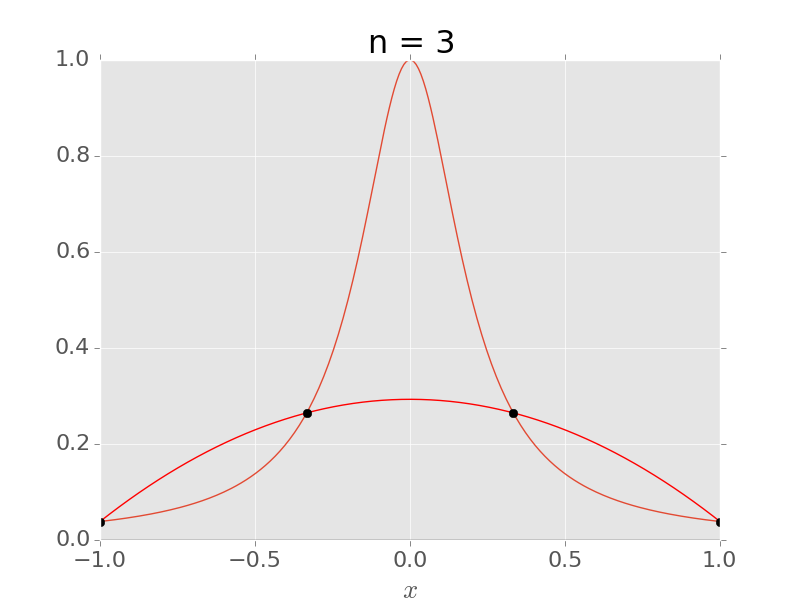
\includegraphics[width=0.45\linewidth,height=\textheight,keepaspectratio]{im/runge1.png}
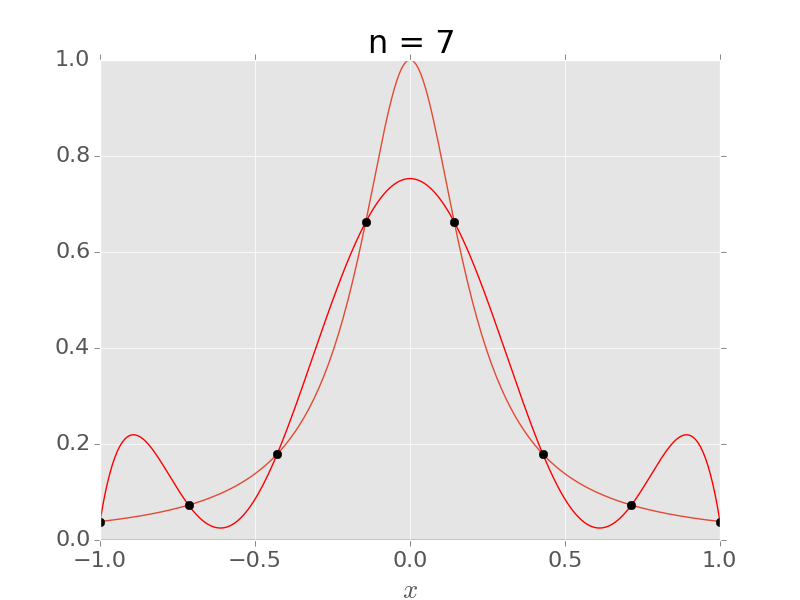
\includegraphics[width=0.45\linewidth,height=\textheight,keepaspectratio]{im/runge2.png}
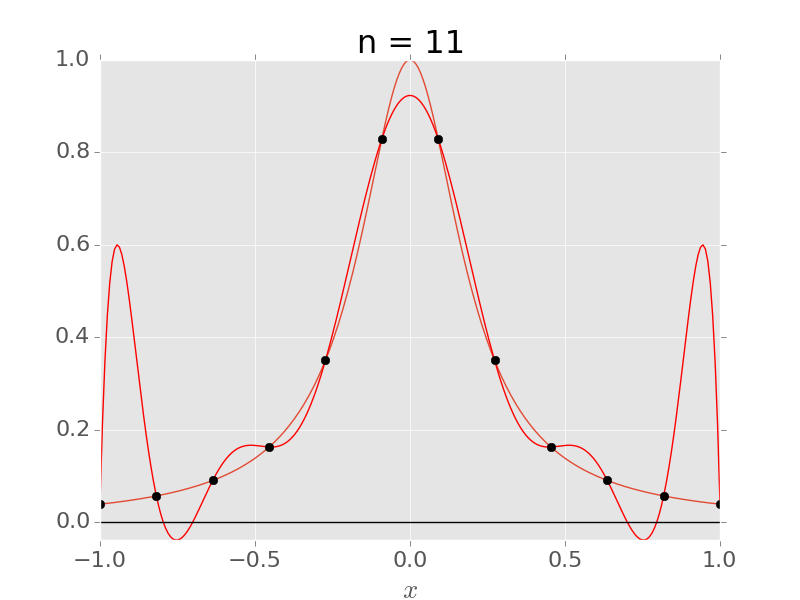
\includegraphics[width=0.45\linewidth,height=\textheight,keepaspectratio]{im/runge3.png}
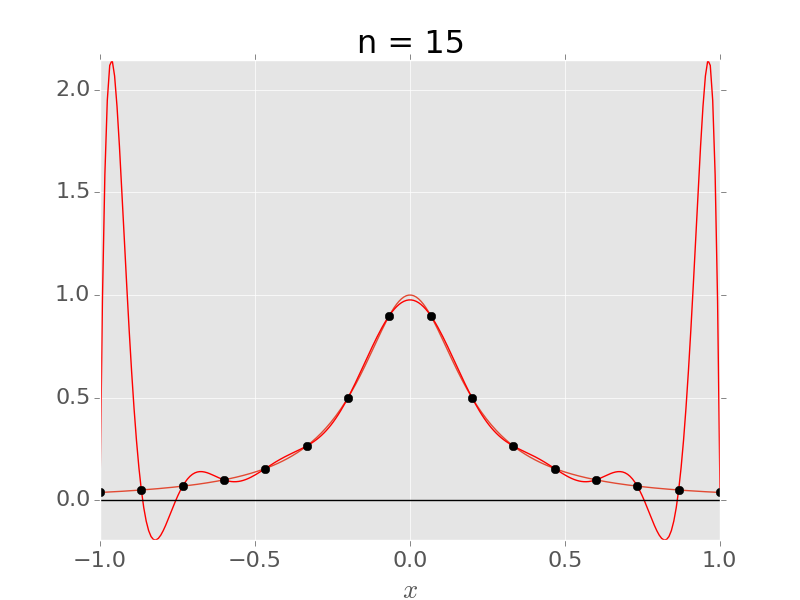
\includegraphics[width=0.45\linewidth,height=\textheight,keepaspectratio]{im/runge4.png}

Notice that \(p_n\) is converging to \(f\) in the middle, but diverging
more and more near the ends, even within the interval \([x_0,x_n]\).
This is called the \textbf{Runge phenomenon}.

\end{fbxSimple}

\begin{tcolorbox}[enhanced jigsaw, bottomrule=.15mm, colbacktitle=quarto-callout-note-color!10!white, breakable, arc=.35mm, coltitle=black, colback=white, bottomtitle=1mm, opacityback=0, title=\textcolor{quarto-callout-note-color}{\faInfo}\hspace{0.5em}{Note}, titlerule=0mm, toptitle=1mm, opacitybacktitle=0.6, colframe=quarto-callout-note-color-frame, leftrule=.75mm, rightrule=.15mm, left=2mm, toprule=.15mm]

A full mathematical explanation for this divergence usually uses complex
analysis --- see Chapter 13 of \emph{Approximation Theory and
Approximation Practice} by L.N. Trefethen (SIAM, 2013). For a more
elementary proof, see
\href{http://math.stackexchange.com/questions/775405/}{this
StackExchange post}.

\end{tcolorbox}

The problem is (largely) coming from the interpolating polynomial \[
w(x) = \prod_{i=0}^n(x-x_i).
\] We can avoid the Runge phenomenon by choosing different nodes \(x_i\)
that are \textbf{not uniformly spaced}.

Since the problems are occurring near the ends of the interval, it would
be logical to put more nodes there. A good choice is given by taking
equally-spaced points on the unit circle \(|z|=1\), and projecting to
the real line:

\begin{center}
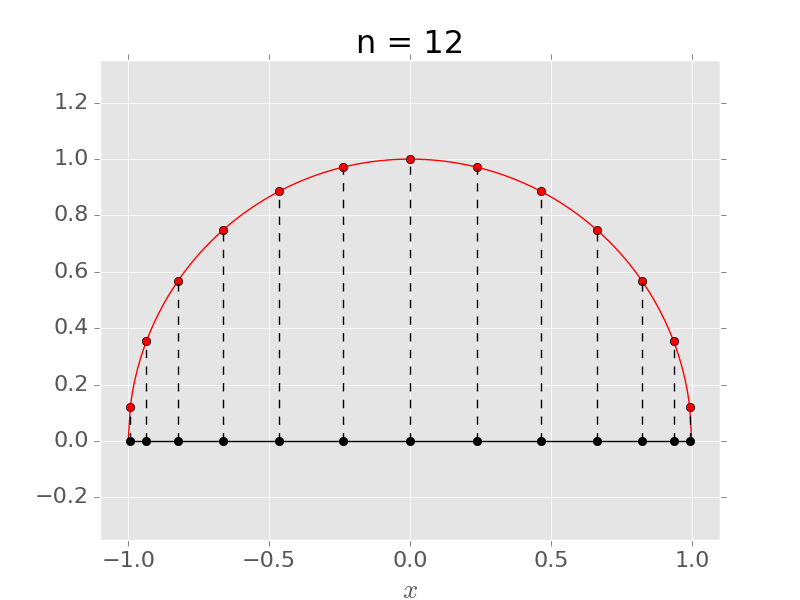
\includegraphics[width=0.6\linewidth,height=\textheight,keepaspectratio]{im/chebnodes.png}
\end{center}

The points around the circle are \[
\phi_j = \frac{(2j+1)\pi}{2(n+1)}, \quad j=0,\ldots,n,
\] so the corresponding \textbf{Chebyshev nodes} are \[
x_j = \cos\left[\frac{(2j + 1)\pi}{2(n+1)}\right], \quad j=0,\ldots,n.
\]

\phantomsection\label{the-runge-function-fx-1125x2-on--11-using-the-chebyshev-nodes.}
\begin{fbxSimple}{eg}{Example 2.10: }{The Runge function \(f(x) = 1/(1+25x^2)\) on \([-1,1]\) using the Chebyshev nodes.}
\phantomsection\label{the-runge-function-fx-1125x2-on--11-using-the-chebyshev-nodes.}
For \(n=3\), the nodes are \(x_0=\cos(\tfrac\pi8)\),
\(x_1=\cos(\tfrac{3\pi}{8})\), \(x_2=\cos(\tfrac{5\pi}{8})\),
\(x_3=\cos(\tfrac{7\pi}{8})\).

Below we illustrate the resulting interpolant for \(n=15\):

\begin{center}
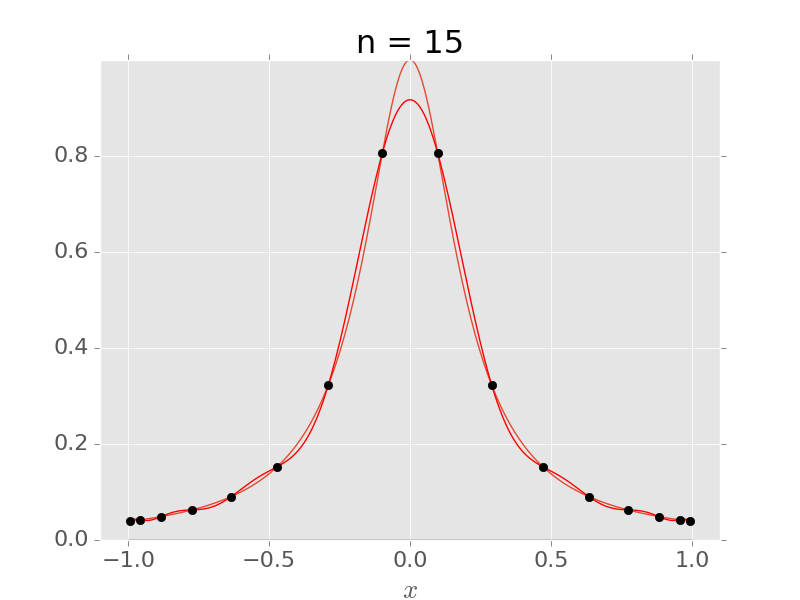
\includegraphics[width=0.5\linewidth,height=\textheight,keepaspectratio]{im/runge_cheby.png}
\end{center}

Compare this to the example with equally spaced nodes.

\end{fbxSimple}

In fact, the Chebyshev nodes are, in one sense, an optimal choice. To
see this, we first note that they are zeroes of a particular polynomial.

The Chebyshev points \(x_j=\cos\left[\frac{(2j+1)\pi}{2(n+1)}\right]\)
for \(j=0,\ldots,n\) are zeroes of the Chebyshev polynomial \[
T_{n+1}(t) := \cos\big[(n+1)\arccos(t)\big]
\]

\begin{tcolorbox}[enhanced jigsaw, bottomrule=.15mm, colbacktitle=quarto-callout-note-color!10!white, breakable, arc=.35mm, coltitle=black, colback=white, bottomtitle=1mm, opacityback=0, title=\textcolor{quarto-callout-note-color}{\faInfo}\hspace{0.5em}{Note}, titlerule=0mm, toptitle=1mm, opacitybacktitle=0.6, colframe=quarto-callout-note-color-frame, leftrule=.75mm, rightrule=.15mm, left=2mm, toprule=.15mm]

The Chebyshev polynomials are denoted \(T_n\) rather than \(C_n\)
because the name is transliterated from Russian as ``Tchebychef'' in
French, for example.

\end{tcolorbox}

In choosing the Chebyshev nodes, we are choosing the error polynomial
\(w(x):=\prod_{i=0}^n(x-x_i)\) to be \(T_{n+1}(x)/2^n\). (This
normalisation makes the leading coefficient 1) This is a good choice
because of the following result.

\phantomsection\label{chebyshev-interpolation}
\begin{fbxSimple}{theorem}{Theorem 2.7: }{Chebyshev interpolation}
\phantomsection\label{chebyshev-interpolation}
Let \(x_0, x_1, \ldots, x_n \in [-1,1]\) be distinct. Then
\(\max_{[-1,1]}|w(x)|\) is minimized if \[
w(x) = \frac{1}{2^n}T_{n+1}(x),
\] where \(T_{n+1}(x)\) is the \textbf{Chebyshev polynomial}
\(T_{n+1}(x) = \cos\Big((n+1)\arccos(x)\Big)\).

\end{fbxSimple}

Having established that the Chebyshev polynomial minimises the maximum
error, we can see convergence as \(n\to\infty\) from the fact that \[
|f(x) - p_n(x)| = \frac{|f^{(n+1)}(\xi)|}{(n+1)!}|w(x)| = \frac{|f^{(n+1)}(\xi)|}{2^n(n+1)!}|T_{n+1}(x)| \leq \frac{|f^{(n+1)}(\xi)|}{2^n(n+1)!}.
\]

If the function is well-behaved enough that \(|f^{(n+1)}(x)| < M\) for
some constant whenever \(x \in [-1,1]\), then the error will tend to
zero as \(n \to \infty\).

\section{Nonlinear Equations}\label{nonlinear-equations}

\begin{quote}
\emph{How do we find roots of nonlinear equations?}
\end{quote}

Given a general equation \[
f(x) = 0,
\] there will usually be no explicit formula for the root(s) \(x_*\), so
we must use an iterative method.

Rootfinding is a delicate business, and it is essential to begin by
plotting a graph of \(f(x)\), so that you can tell whether the answer
you get from your numerical method is correct.

\phantomsection\label{fx-frac1x---a-for-a-0.}
\begin{fbxSimple}{eg}{Example 2.11: }{\(f(x) = \frac{1}{x} - a\), for \(a > 0\).}
\phantomsection\label{fx-frac1x---a-for-a-0.}
\begin{center}
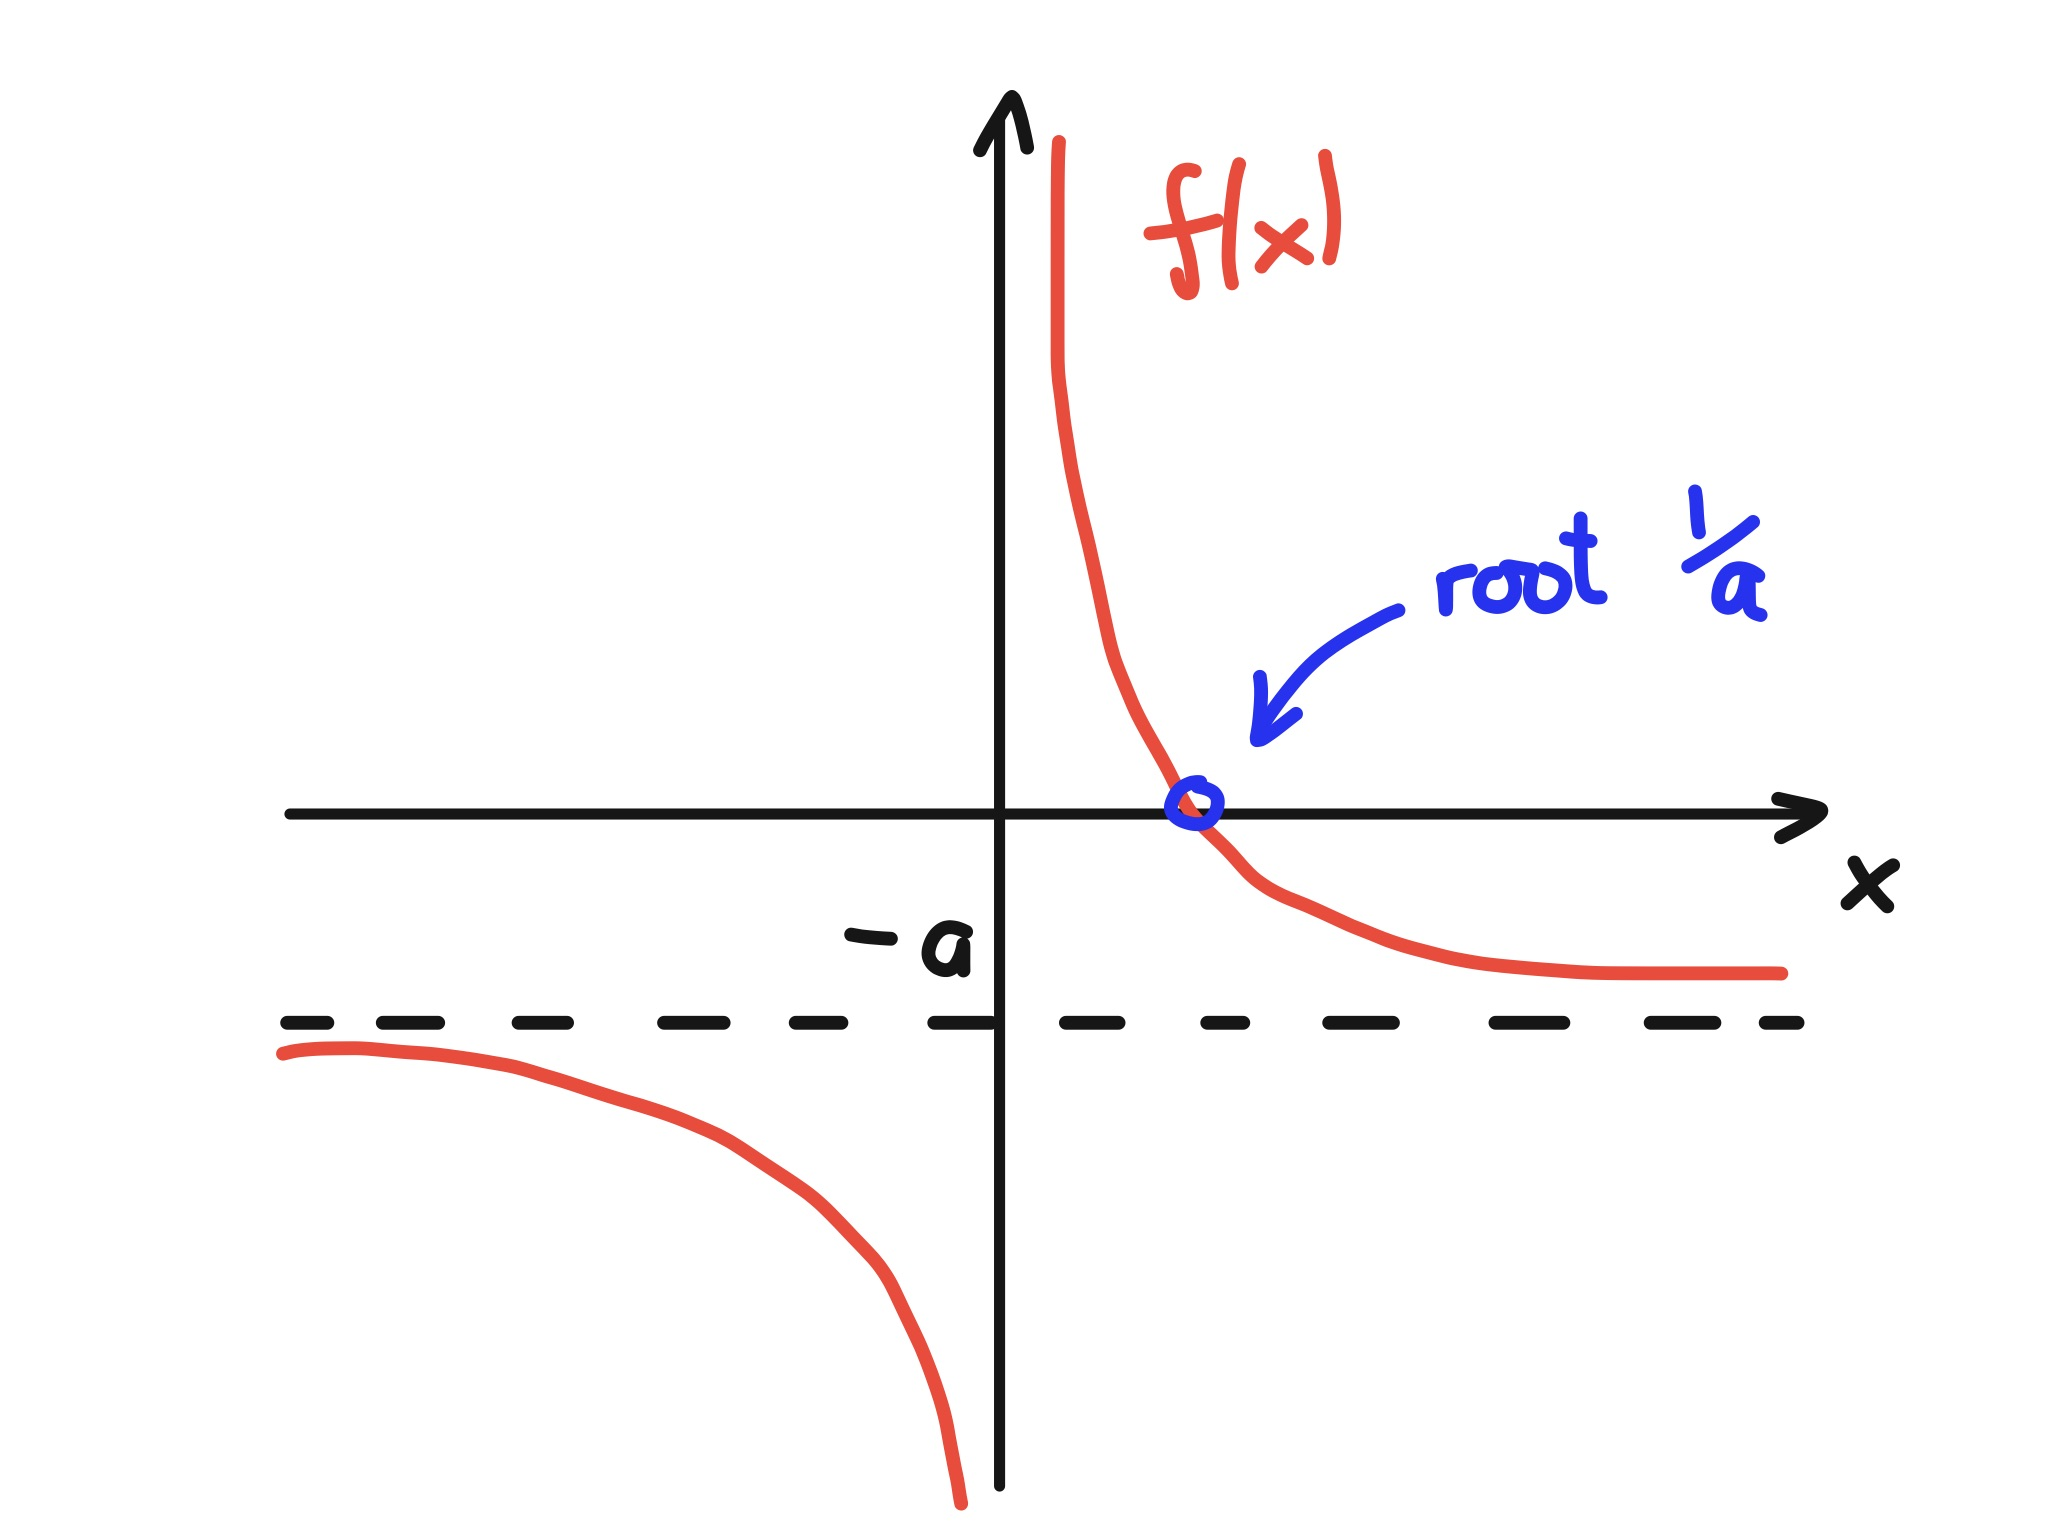
\includegraphics[width=0.6\linewidth,height=\textheight,keepaspectratio]{im/root1.jpg}
\end{center}

Clearly we know the root is exactly \(x_* = \frac{1}{a}\), but this will
serve as a running example to test some of our methods

\end{fbxSimple}

\subsection{Interval Bisection}\label{interval-bisection}

If \(f\) is continuous and we can find an interval where it changes
sign, then it must have a root in this interval. Formally, this is based
on:

\phantomsection\label{intermediate-value-theorem}
\begin{fbxSimple}{theorem}{Theorem 2.8: }{Intermediate Value Theorem}
\phantomsection\label{intermediate-value-theorem}
If \(f\) is continuous on \([a,b]\) and \(c\) lies between \(f(a)\) and
\(f(b)\), then there is at least one point \(x\in[a,b]\) such that
\(f(x)=c\).

\end{fbxSimple}

If \(f(a)f(b)<0\), then \(f\) changes sign at least once in \([a,b]\),
so by the Intermediate Value Theorem there must be a point
\(x_*\in[a,b]\) where \(f(x_*)=0\).

We can turn this into the following iterative algorithm:

\phantomsection\label{algorithm-2.1}
\begin{fbxSimple}{algorithm}{Algorithm 2.1: }{Interval bisection}
\phantomsection\label{algorithm-2.1}

Let \(f\) be continuous on \([a_0,b_0]\), with \(f(a_0)f(b_0)<0\).

\begin{itemize}
\tightlist
\item
  At each step, set \(m_k = (a_k + b_k)/2\).
\item
  If \(f(a_k)f(m_k)\geq 0\) then set \(a_{k+1}=m_k\), \(b_{k+1}=b_k\),
  otherwise set \(a_{k+1}=a_k\), \(b_{k+1}=m_k\).
\end{itemize}

\end{fbxSimple}

\phantomsection\label{fxtfrac1x---0.5.}
\begin{fbxSimple}{eg}{Example 2.12: }{\(f(x)=\tfrac1x - 0.5\).}
\phantomsection\label{fxtfrac1x---0.5.}

\begin{enumerate}
\def\labelenumi{\arabic{enumi}.}
\item
  Try \(a_0=1\), \(b_0=3\) so that \(f(a_0)f(b_0)=0.5(-0.1666) < 0\).\\
  Now the midpoint is \(m_0=(1 + 3)/2 = 2\), with \(f(m_0)=0\).\\
  We are lucky and have already stumbled on the root \(x_*=m_0=2\)!
\item
  Suppose we had tried \(a_0=1.5\), \(b_0=3\), so \(f(a_0)=0.1666\) and
  \(f(b_0)=-0.1666\), and again \(f(a_0)f(b_0)<0\).\\
  Now \(m_0 = 2.25\), \(f(m_0)=-0.0555\). We have \(f(a_0)f(m_0) < 0\),
  so we set \(a_1 = a_0=1.5\) and \(b_1 = m_0=2.25\). The root must lie
  in \([1.5,2.25]\).\\
  Now \(m_1 = 1.875\), \(f(m_1)=0.0333\), and \(f(a_1)f(m_1)>0\), so we
  take \(a_2 = m_1=1.875\), \(b_2 = b_1=2.25\). The root must lie in
  \([1.875,2.25]\).\\
  We can continue this algorithm, halving the length of the interval
  each time.
\end{enumerate}

\end{fbxSimple}

Since the interval halves in size at each iteration, and always contains
a root, we are guaranteed to converge to a root provided that \(f\) is
continuous. Stopping at step \(k\), we get the minimum possible error by
choosing \(m_k\) as our approximation.

\phantomsection\label{same-example-with-initial-interval--0.50.5.}
\begin{fbxSimple}{eg}{Example 2.13: }{Same example with initial interval \([-0.5,0.5]\).}
\phantomsection\label{same-example-with-initial-interval--0.50.5.}
\begin{center}
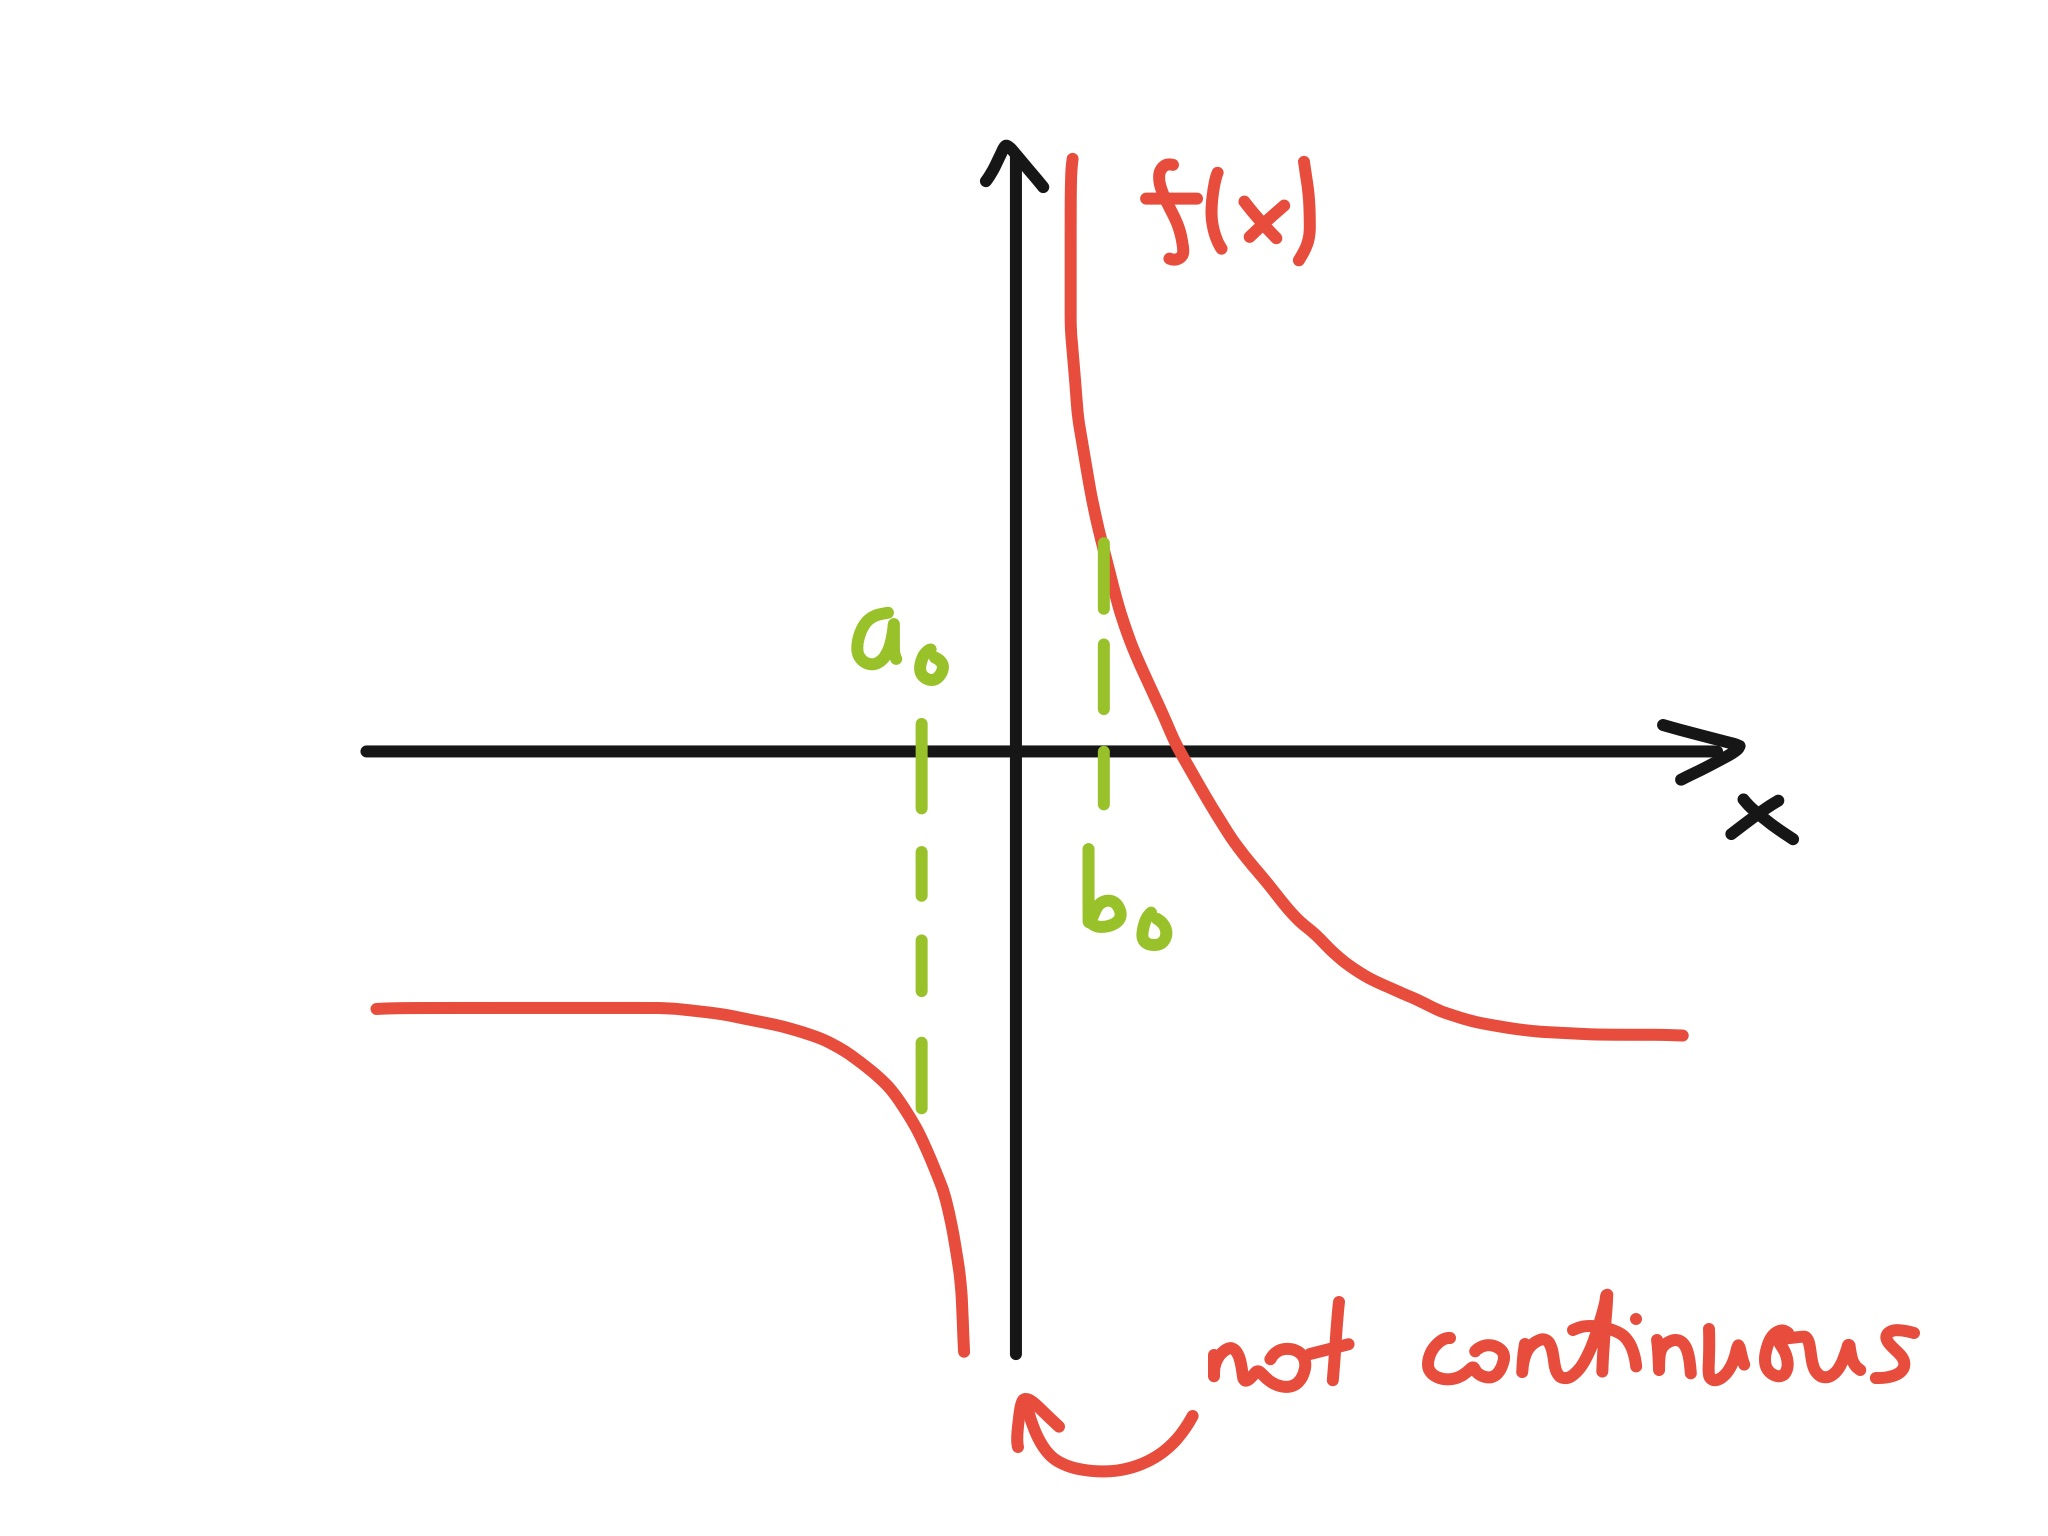
\includegraphics[width=0.7\linewidth,height=\textheight,keepaspectratio]{im/root2.jpg}
\end{center}

In this case \(f(a_0)f(b_0)<0\), but there is no root in the interval.

\end{fbxSimple}

The rate of convergence is steady, so we can pre-determine how many
iterations will be needed to converge to a given accuracy. After \(k\)
iterations, the interval has length \[
|b_k - a_k| = \frac{|b_0 - a_0|}{2^k},
\] so the error in the mid-point satisfies \[
|m_k - x_*| \leq \frac{|b_0 - a_0|}{2^{k+1}}.
\] In order for \(|m_k - x_*| \leq \delta\), we need \(n\) iterations,
where \[
\frac{|b_0 - a_0|}{2^{n+1}} \leq \delta \quad \implies \log|b_0-a_0| - (n+1)\log(2) \leq \log(\delta) \quad \implies n \geq \frac{\log|b_0-a_0| - \log(\delta)}{\log(2)} - 1.
\]

\phantomsection\label{previous-example-continued}
\begin{fbxSimple}{eg}{Example 2.14: }{Previous example continued}
\phantomsection\label{previous-example-continued}
With \(a_0=1.5\), \(b_0=3\), as in the above example, then for
\(\delta = \epsilon_{\rm M}=1.1\times 10^{-16}\) we would need \[
n \geq \frac{\log(1.5) - \log(1.1\times 10^{-16})}{\log(2)}-1 \quad \implies n \geq 53 \textrm{ iterations}.
\]

\end{fbxSimple}

\begin{tcolorbox}[enhanced jigsaw, bottomrule=.15mm, colbacktitle=quarto-callout-note-color!10!white, breakable, arc=.35mm, coltitle=black, colback=white, bottomtitle=1mm, opacityback=0, title=\textcolor{quarto-callout-note-color}{\faInfo}\hspace{0.5em}{Note}, titlerule=0mm, toptitle=1mm, opacitybacktitle=0.6, colframe=quarto-callout-note-color-frame, leftrule=.75mm, rightrule=.15mm, left=2mm, toprule=.15mm]

This convergence is pretty slow, but the method has the advantage of
being very robust (i.e., use it if all else fails\ldots). It has the
more serious disadvantage of \emph{only working in one dimension}.

\end{tcolorbox}

\subsection{Fixed point iteration}\label{fixed-point-iteration}

This is a very common type of rootfinding method. The idea is to
transform \(f(x)=0\) into the form \(g(x)=x\), so that a root \(x_*\) of
\(f\) is a \textbf{fixed point} of \(g\), meaning \(g(x_*)=x_*\). To
find \(x_*\), we start from some initial guess \(x_0\) and iterate \[
x_{k+1} = g(x_k)
\] until \(|x_{k+1}-x_k|\) is sufficiently small. For a given equation
\(f(x)=0\), there are many ways to transform it into the form
\(x=g(x)\). Only some will result in a convergent iteration.

\phantomsection\label{fxx2-2x-3.}
\begin{fbxSimple}{eg}{Example 2.15: }{\(f(x)=x^2-2x-3\).}
\phantomsection\label{fxx2-2x-3.}
Note that the roots are \(-1\) and \(3\). Consider some different
rearrangements, with \(x_0=0\).

\begin{enumerate}
\def\labelenumi{\arabic{enumi}.}
\item
  \(g(x) = \sqrt{2x+3}\), gives \(x_k\to 3\) {[}to machine accuracy
  after 33 iterations{]}.
\item
  \(g(x) = 3/(x-2)\), gives \(x_k\to -1\) {[}to machine accuracy after
  33 iterations{]}.
\item
  \(g(x) = (x^2 - 3)/2\), gives \(x_k\to -1\) {[}but very slowly!{]}.
\item
  \(g(x) = x^2 - x - 3\), gives \(x_k\to\infty\).
\item
  \(g(x) = (x^2+3)/(2x-2)\), gives \(x_k\to -1\) {[}to machine accuracy
  after 5 iterations{]}.
\end{enumerate}

If instead we take \(x_0=42\), then (1) and (2) still converge to the
same roots, (3) now diverges, (4) still diverges, and (5) now converges
to the other root \(x_k\to 3\).

\end{fbxSimple}

In this section, we will consider which iterations will converge, before
addressing the \emph{rate} of convergence in Section~\ref{sec-order}.

One way to ensure that the iteration will work is to find a
\textbf{contraction mapping} \(g\), which is a map \(L\to L\) (for some
closed interval \(L\)) satisfying \[
|g(x)-g(y)| \leq \lambda|x-y|
\] for some \(\lambda < 1\) and for all \(x\), \(y \in L\). The sketch
below shows the idea:

\begin{center}
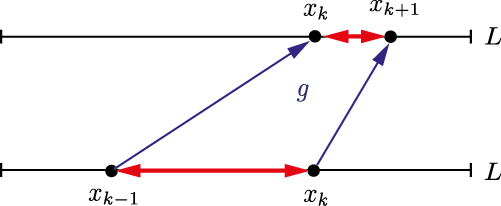
\includegraphics[width=0.7\linewidth,height=\textheight,keepaspectratio]{im/contraction.png}
\end{center}

\phantomsection\label{contraction-mapping-theorem}
\begin{fbxSimple}{theorem}{Theorem 2.9: }{Contraction Mapping Theorem}
\phantomsection\label{contraction-mapping-theorem}
If \(g\) is a contraction mapping on \(L=[a,b]\), then 1. There exists a
unique fixed point \(x_*\in L\) with \(g(x_*)=x_*\). 2. For any
\(x_0\in L\), the iteration \(x_{k+1}=g(x_k)\) will converge to \(x_*\)
as \(k\to\infty\).

\end{fbxSimple}

\textbf{Proof:}\\
To prove \emph{existence}, consider \(h(x)=g(x)-x\). Since \(g:L\to L\)
we have \(h(a)=g(a)-a\geq 0\) and \(h(b)=g(b)-b\leq 0\). Moreover, it
follows from the contraction property above that \(g\) is continuous
(think of ``\(\epsilon\delta\)''), therefore so is \(h\). So the
Intermediate Value Theorem guarantees the existence of at least one
point \(x_*\in L\) such that \(h(x_*)=0\), i.e.~\(g(x_*)=x_*\).

For \emph{uniqueness}, suppose \(x_*\) and \(y_*\) are both fixed points
of \(g\) in \(L\). Then \[
|x_*-y_*| = |g(x_*)-g(y_*)| \leq \lambda |x_*-y_*| < |x_*-y_*|,
\] which is a contradiction.

Finally, to show \emph{convergence}, consider \[
|x_*- x_{k+1} | = |g(x_*) - g(x_k)| \leq \lambda |x_* - x_k| \leq \ldots \leq \lambda^{k+1}|x_*-x_0|.
\] Since \(\lambda<1\), we see that \(x_k\to x_*\) as \(k\to\infty\).

\begin{tcolorbox}[enhanced jigsaw, bottomrule=.15mm, colbacktitle=quarto-callout-note-color!10!white, breakable, arc=.35mm, coltitle=black, colback=white, bottomtitle=1mm, opacityback=0, title=\textcolor{quarto-callout-note-color}{\faInfo}\hspace{0.5em}{Note}, titlerule=0mm, toptitle=1mm, opacitybacktitle=0.6, colframe=quarto-callout-note-color-frame, leftrule=.75mm, rightrule=.15mm, left=2mm, toprule=.15mm]

The Contraction Mapping Theorem is also known as the \textbf{Banach
fixed point theorem}, and was proved by Stefan Banach in his 1920 PhD
thesis.

\end{tcolorbox}

To apply this result in practice, we need to know whether a given
function \(g\) is a contraction mapping on some interval.

If \(g\) is differentiable, then Taylor's theorem says that there exists
\(\xi\in(x,y)\) with \[
g(x) = g(y) + g'(\xi)(x-y) \,\, \implies \,\, |g(x)-g(y)| \leq \Big(\max_{\xi\in L}|g'(\xi)|\Big)\,|x-y|.
\] So if (a) \(g:L\to L\) and (b) \(|g'(x)|\leq M\) for all \(x\in L\)
with \(M<1\), then \(g\) is a contraction mapping on \(L\).

\phantomsection\label{iteration-a-from-previous-example-gx-sqrt2x-3.}
\begin{fbxSimple}{eg}{Example 2.16: }{Iteration (a) from previous example, \(g(x) = \sqrt{2x + 3}\).}
\phantomsection\label{iteration-a-from-previous-example-gx-sqrt2x-3.}
Here \(g'=(2x + 3)^{-1/2}\), so we see that \(|g'(x)|<1\) for all
\(x>-1\).

For \(g\) to be a contraction mapping on an interval \(L\), we also need
that \(g\) maps \(L\) into itself. Since our particular \(g\) is
continuous and monotonic increasing (for \(x>-\tfrac32\)), it will map
an interval \([a,b]\) to another interval whose end-points are \(g(a)\)
and \(g(b)\).

For example, \(g(-\tfrac12)=\sqrt{2}\) and \(g(4)=\sqrt{11}\), so the
interval \(L=[-\tfrac12,4]\) is mapped into itself. It follows by the
Contraction Mapping Theorem that (1) there is a unique fixed point
\(x_*\in[-\tfrac12,4]\) (which we know is \(x_*=3\)), and (2) the
iteration will converge to \(x_*\) for any \(x_0\) in this interval (as
we saw for \(x_0=0\)).

\end{fbxSimple}

In practice, it is not always easy to find a suitable interval \(L\).
But knowing that \(|g'(x_*)|<1\) is enough to guarantee that the
iteration will converge if \(x_0\) is close enough to \(x_*\).

\phantomsection\label{local-convergence-theorem}
\begin{fbxSimple}{theorem}{Theorem 2.10: }{Local Convergence Theorem}
\phantomsection\label{local-convergence-theorem}
Let \(g\) and \(g'\) be continuous in the neighbourhood of an isolated
fixed point \(x_*=g(x_*)\). If \(|g'(x_*)|<1\) then there is an interval
\(L=[x_*-\delta,x_*+\delta]\) such that \(x_{k+1}=g(x_k)\) converges to
\(x_*\) whenever \(x_0\in L\).

\end{fbxSimple}

\textbf{Proof:}\\
By continuity of \(g'\), there exists some interval
\(L=[x_*-\delta,x_*+\delta]\) with \(\delta>0\) such that \(|g'(x)|\leq
M\) for some \(M<1\), for all \(x\in L\). Now let \(x\in L\). It follows
that \[
|x_* - g(x)| = |g(x_*)-g(x)| \leq M|x_*-x| < |x_*-x| \leq \delta,
\] so \(g(x)\in L\). Hence \(g\) is a contraction mapping on \(L\) and
the Contraction Mapping Theorem shows that \(x_k\to x_*\).

\phantomsection\label{iteration-a-again-gx-sqrt2x-3.}
\begin{fbxSimple}{eg}{Example 2.17: }{Iteration (a) again, \(g(x) = \sqrt{2x + 3}\).}
\phantomsection\label{iteration-a-again-gx-sqrt2x-3.}
Here we know that \(x_*=3\), and \(|g'(3)|=\tfrac13 < 1\), so the Local
Convergence Theorem tells us that the iteration will converge to \(3\)
if \(x_0\) is close enough to \(3\).

\end{fbxSimple}

\phantomsection\label{iteration-e-again-gx-x232x-2.}
\begin{fbxSimple}{eg}{Example 2.18: }{Iteration (e) again, \(g(x) = (x^2+3)/(2x-2)\).}
\phantomsection\label{iteration-e-again-gx-x232x-2.}
Here we have \[
g'(x) = \frac{x^2-2x-3}{2(x-1)^2},
\] so we see that \(g'(-1)=g'(3)=0 < 1\). So the Local Convergence
Theorem tells us that the iteration will converge to either root if we
start close enough.

\end{fbxSimple}

\begin{tcolorbox}[enhanced jigsaw, bottomrule=.15mm, colbacktitle=quarto-callout-note-color!10!white, breakable, arc=.35mm, coltitle=black, colback=white, bottomtitle=1mm, opacityback=0, title=\textcolor{quarto-callout-note-color}{\faInfo}\hspace{0.5em}{Note}, titlerule=0mm, toptitle=1mm, opacitybacktitle=0.6, colframe=quarto-callout-note-color-frame, leftrule=.75mm, rightrule=.15mm, left=2mm, toprule=.15mm]

As we will see, the fact that \(g'(x_*)=0\) is related to the fast
convergence of iteration (e).

\end{tcolorbox}

\subsection{Orders of convergence}\label{sec-order}

To measure the speed of convergence, we compare the error
\(|x_*-x_{k+1}|\) to the error at the previous step, \(|x_*-x_k|\).

\phantomsection\label{eg-2.19}
\begin{fbxSimple}{eg}{Example 2.19: }{Interval bisection.}
\phantomsection\label{eg-2.19}
Here we had \(|x_*-m_{k+1}| \leq \tfrac12|x_*-m_k|\). This is called
\textbf{linear convergence}, meaning that we have
\(|x_*-x_{k+1}|\leq \lambda |x_* - x_{k}|\) for some constant
\(\lambda < 1\).

\end{fbxSimple}

We can compare a few different iteration schemes that should converge to
the same answer to get a sense for how our choice of scheme can impact
the convergence order.

\phantomsection\label{iteration-a-again-gxsqrt2x3.}
\begin{fbxSimple}{eg}{Example 2.20: }{Iteration (a) again, \(g(x)=\sqrt{2x+3}\).}
\phantomsection\label{iteration-a-again-gxsqrt2x3.}
Look at the sequence of errors in this case:

\begin{longtable}[]{@{}lll@{}}
\toprule\noalign{}
\(x_k\) & \(|3-x_k|\) & \(|3-x_k|/|3-x_{k-1}|\) \\
\midrule\noalign{}
\endhead
\bottomrule\noalign{}
\endlastfoot
0.0000000000 & 3.0000000000 & - \\
1.7320508076 & 1.2679491924 & 0.4226497308 \\
2.5424597568 & 0.4575402432 & 0.3608506129 \\
2.8433992885 & 0.1566007115 & 0.3422665304 \\
2.9473375404 & 0.0526624596 & 0.3362849319 \\
2.9823941860 & 0.0176058140 & 0.3343143126 \\
2.9941256440 & 0.0058743560 & 0.3336600063 \\
\end{longtable}

We see that the ratio \(|x_*-x_k|/|x_*-x_{k-1}|\) is indeed less than
\(1\), and seems to be converging to \(\lambda\approx\tfrac13\). So this
is a linearly convergent iteration.

\end{fbxSimple}

\phantomsection\label{iteration-e-again-gx-x232x-2.-1}
\begin{fbxSimple}{eg}{Example 2.21: }{Iteration (e) again, \(g(x) = (x^2+3)/(2x-2)\).}
\phantomsection\label{iteration-e-again-gx-x232x-2.-1}
Now the sequence is:

\begin{longtable}[]{@{}lll@{}}
\toprule\noalign{}
\(x_k\) & \(|(-1)-x_k|\) & \(|(-1)-x_k|/|(-1)-x_{k-1}|\) \\
\midrule\noalign{}
\endhead
\bottomrule\noalign{}
\endlastfoot
0.0000000000 & 1.0000000000 & - \\
-1.5000000000 & 0.5000000000 & 0.5000000000 \\
-1.0500000000 & 0.0500000000 & 0.1000000000 \\
-1.0006097561 & 0.0006097561 & 0.0121951220 \\
-1.0000000929 & 0.0000000929 & 0.0001523926 \\
\end{longtable}

Again the ratio \(|x_*-x_{k}|/|x_*-x_{k-1}|\) is certainly less than
\(1\), but this time we seem to have \(\lambda\to 0\) as \(k\to\infty\).
This is called \textbf{superlinear convergence}, meaning that the
convergence is in some sense ``accelerating''.

\end{fbxSimple}

In general, if \(x_k\to x_*\) then we say that the sequence \(\{x_k\}\)
\textbf{converges linearly} if \[
\lim_{k\to\infty}\frac{|x_*-x_{k+1}|}{|x_*-x_k|} = \lambda \quad \textrm{with} \quad 0<\lambda <1.
\] If \(\lambda=0\) then the convergence is \textbf{superlinear}.

\begin{tcolorbox}[enhanced jigsaw, bottomrule=.15mm, colbacktitle=quarto-callout-note-color!10!white, breakable, arc=.35mm, coltitle=black, colback=white, bottomtitle=1mm, opacityback=0, title=\textcolor{quarto-callout-note-color}{\faInfo}\hspace{0.5em}{Note}, titlerule=0mm, toptitle=1mm, opacitybacktitle=0.6, colframe=quarto-callout-note-color-frame, leftrule=.75mm, rightrule=.15mm, left=2mm, toprule=.15mm]

The constant \(\lambda\) is called the \textbf{rate} or \textbf{ratio}.

\end{tcolorbox}

The following result establishes conditions for linear and superlinear
convergence.

\phantomsection\label{theorem-2.11}
\begin{fbxSimple}{theorem}{Theorem 2.11}{}
\phantomsection\label{theorem-2.11}

Let \(g'\) be continuous in the neighbourhood of a fixed point
\(x_*=g(x_*)\), and suppose that \(x_{k+1}=g(x_k)\) converges to \(x_*\)
as \(k\to\infty\).

\begin{enumerate}
\def\labelenumi{\arabic{enumi}.}
\item
  If \(|g'(x_*)|\neq 0\) then the convergence will be linear with rate
  \(\lambda=|g'(x_*)|\).
\item
  If \(|g'(x_*)|=0\) then the convergence will be superlinear.
\end{enumerate}

\end{fbxSimple}

\textbf{Proof:}\\
By Taylor's theorem, note that \[
x_* - x_{k+1} = g(x_*) - g(x_k) = g(x_*) - \Big[g(x_*) + g'(\xi_k)(x_k-x_*)\Big] = g'(\xi_k)(x_* - x_k)
\] for some \(\xi_k\) between \(x_*\) and \(x_k\). Since \(x_k\to x_*\),
we have \(\xi_k\to x_*\) as \(k\to\infty\), so \[
\lim_{k\to\infty}\frac{|x_*-x_{k+1}|}{|x_*-x_k|} = \lim_{k\to\infty}|g'(\xi_k)| = |g'(x_*)|.
\] This proves the result.

\phantomsection\label{iteration-a-again-gxsqrt2x3.-1}
\begin{fbxSimple}{eg}{Example 2.22: }{Iteration (a) again, \(g(x)=\sqrt{2x+3}\).}
\phantomsection\label{iteration-a-again-gxsqrt2x3.-1}
We saw before that \(g'(3)=\tfrac13\), so the theorem above shows that
convergence will be linear with \(\lambda = |g'(3)| = \tfrac13\) as we
found numerically.

\end{fbxSimple}

\phantomsection\label{iteration-e-again-gx-x232x-2.-2}
\begin{fbxSimple}{eg}{Example 2.23: }{Iteration (e) again, \(g(x) = (x^2+3)/(2x-2)\).}
\phantomsection\label{iteration-e-again-gx-x232x-2.-2}
We saw that \(g'(-1)=0\), so the theorem above shows that convergence
will be superlinear, again consistent with our numerical findings.

\end{fbxSimple}

We can further classify superlinear convergence by the \textbf{order of
convergence}, defined as \[
\alpha = \sup\left\{\beta \, : \, \lim_{k\to\infty}\frac{|x_*-x_{k+1}|}{|x_*-x_k|^\beta} < \infty \right\}.
\]

For example, \(\alpha=2\) is called \textbf{quadratic} convergence and
\(\alpha=3\) is called \textbf{cubic} convergence, although for a
general sequence \(\alpha\) need not be an integer (e.g.~the secant
method below).

\subsection{Newton's method}\label{newtons-method}

This is a particular fixed point iteration that is very widely used
because (as we will see) it usually converges superlinearly.

\begin{center}
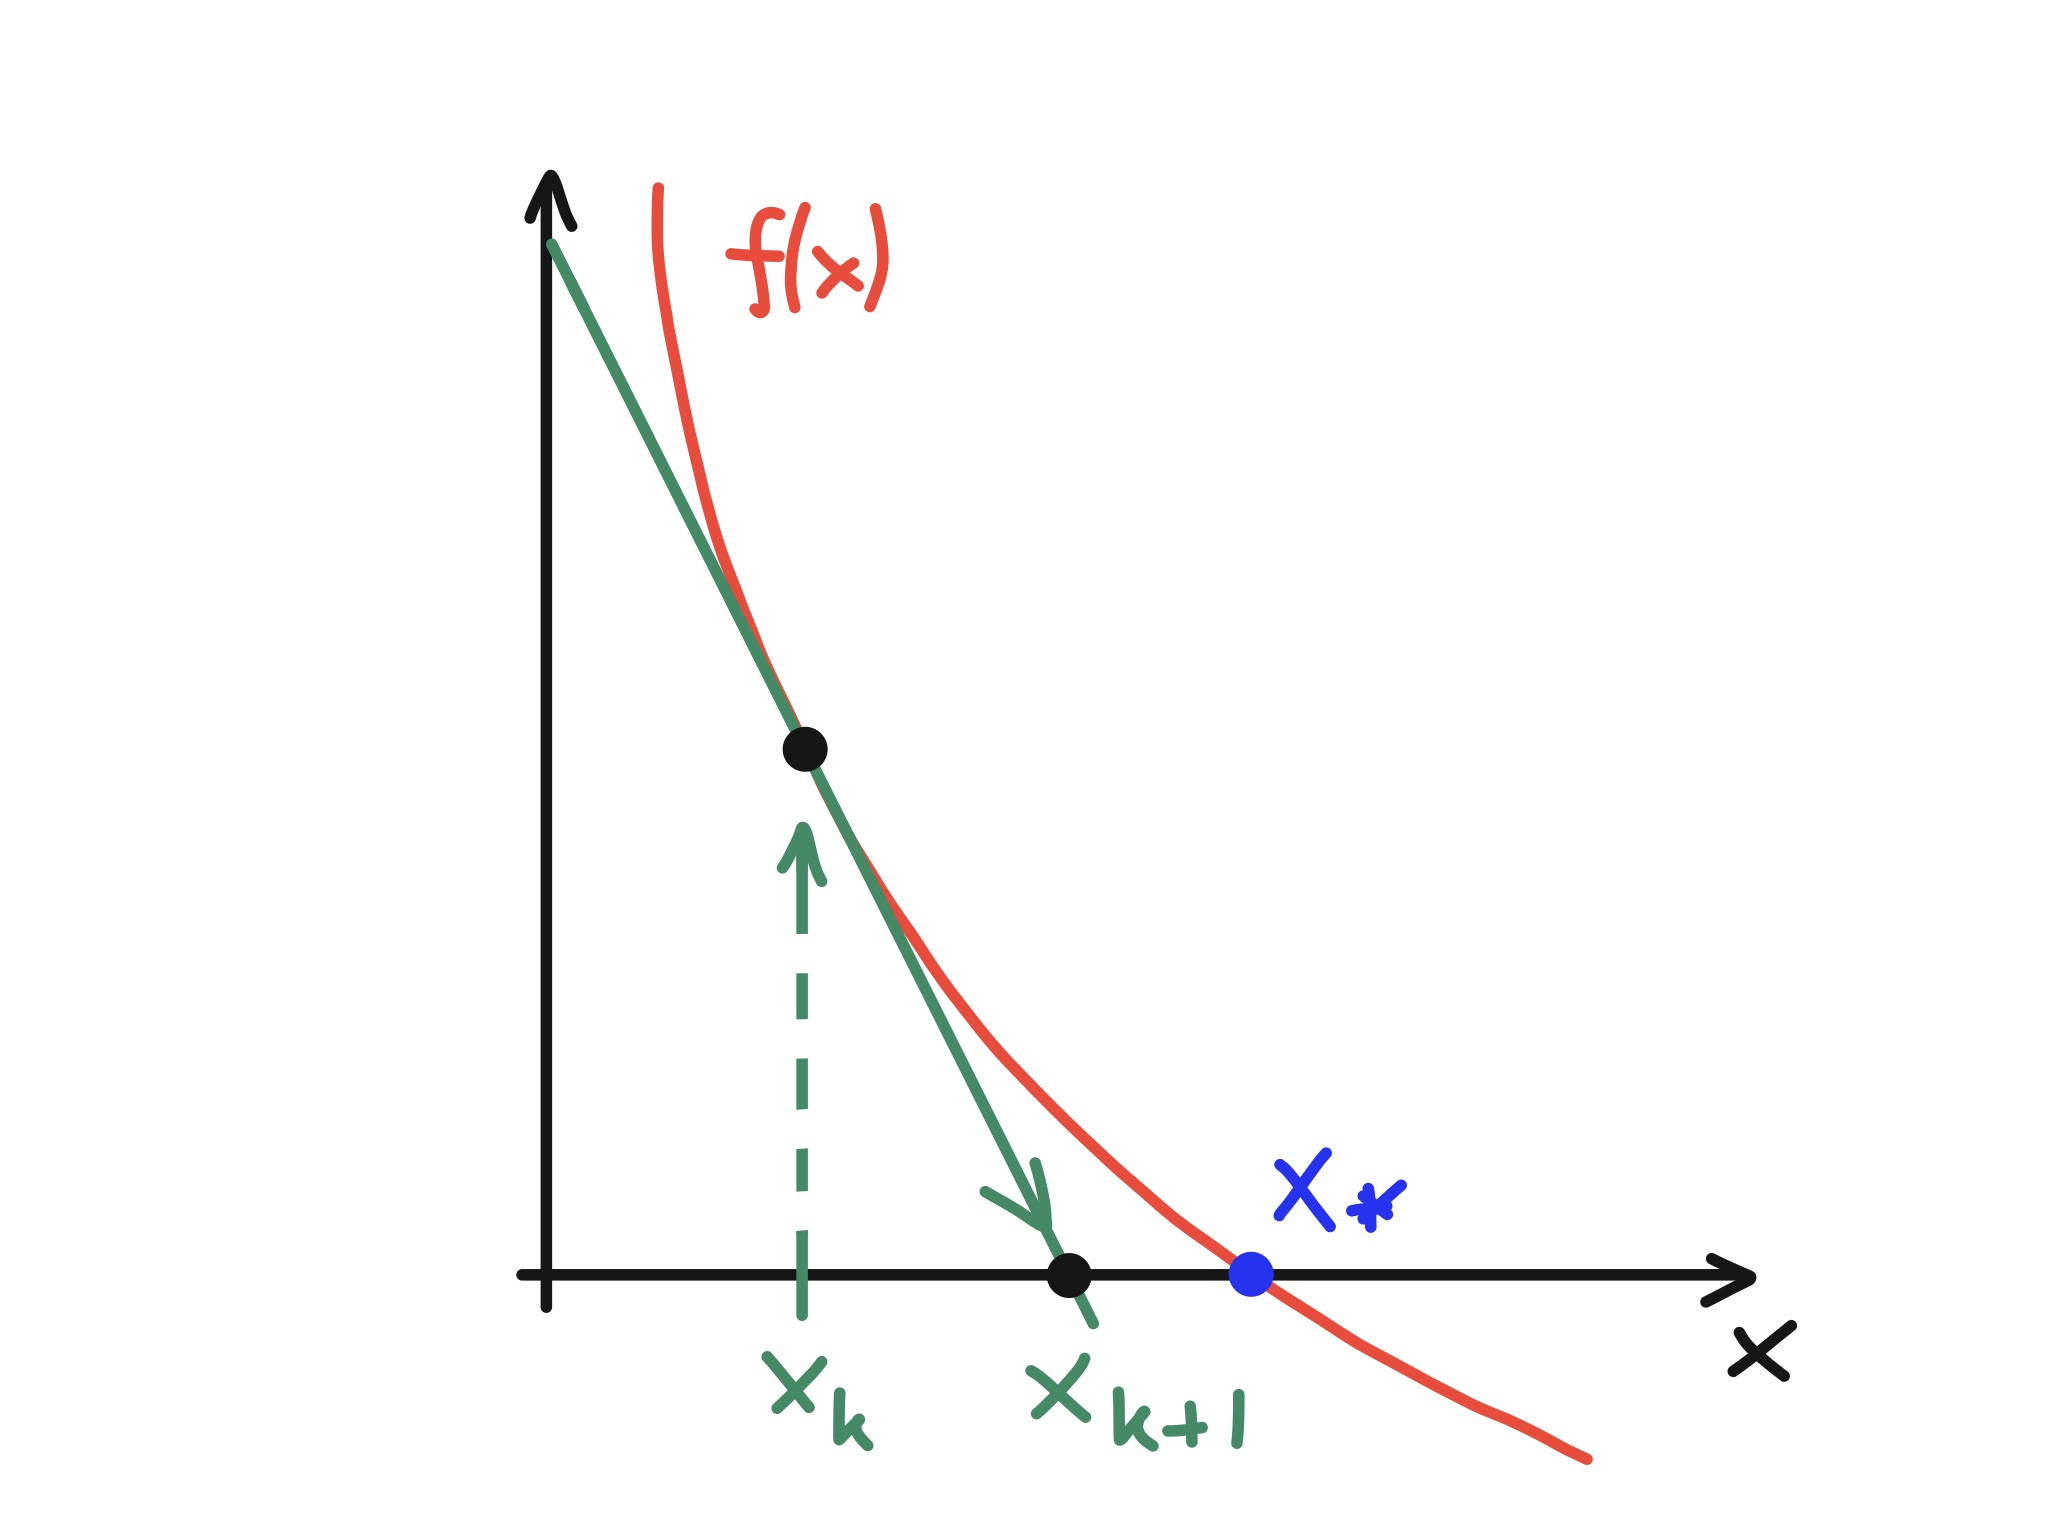
\includegraphics[width=0.7\linewidth,height=\textheight,keepaspectratio]{im/newton.jpg}
\end{center}

Graphically, the idea of \textbf{Newton's method} is simple: given
\(x_k\), draw the tangent line to \(f\) at \(x=x_k\), and let
\(x_{k+1}\) be the \(x\)-intercept of this tangent. So \[
\frac{0 - f(x_k)}{x_{k+1} - x_k} = f'(x_k) \quad \implies\quad  x_{k+1} = x_k - \frac{f(x_k)}{f'(x_k)}.
\]

\begin{tcolorbox}[enhanced jigsaw, bottomrule=.15mm, colbacktitle=quarto-callout-note-color!10!white, breakable, arc=.35mm, coltitle=black, colback=white, bottomtitle=1mm, opacityback=0, title=\textcolor{quarto-callout-note-color}{\faInfo}\hspace{0.5em}{Note}, titlerule=0mm, toptitle=1mm, opacitybacktitle=0.6, colframe=quarto-callout-note-color-frame, leftrule=.75mm, rightrule=.15mm, left=2mm, toprule=.15mm]

In fact, Newton only applied the method to polynomial equations, and
without using calculus. The general form using derivatives
(``fluxions'') was first published by Thomas Simpson in 1740. {[}See
``Historical Development of the Newton-Raphson Method'' by T.J. Ypma,
\emph{SIAM Review} \textbf{37}, 531 (1995).{]}

\end{tcolorbox}

Another way to derive this iteration is to approximate \(f(x)\) by the
linear part of its Taylor series centred at \(x_k\): \[
0 \approx f(x_{k+1}) \approx f(x_k) + f'(x_k)(x_{k+1} - x_{k}).
\]

The iteration function for Newton's method is \[
g(x) = x - \frac{f(x)}{f'(x)},
\] so using \(f(x_*)=0\) we see that \(g(x_*)=x_*\). To assess the
convergence, note that \[
g'(x) = 1 - \frac{f'(x)f'(x) - f(x)f''(x)}{[f'(x)]^2} = \frac{f(x)f''(x)}{[f'(x)]^2} \quad \implies g'(x_*)=0 \quad \textrm{if $f'(x_*)\neq 0$}.
\] So if \(f'(x_*)\neq 0\), the Local Convergence Theorem shows that the
iteration will converge for \(x_0\) close enough to \(x_*\). Moreover,
since \(g'(x_*)=0\), the order theorem shows that this convergence will
be superlinear.

\phantomsection\label{calculate-a-1-using-fxfrac1x---a-for-a0.}
\begin{fbxSimple}{eg}{Example 2.24: }{Calculate \(a^{-1}\) using \(f(x)=\frac1x - a\) for \(a>0\).}
\phantomsection\label{calculate-a-1-using-fxfrac1x---a-for-a0.}
Newton's method gives the iterative formula \[
x_{k+1} = x_k - \frac{\frac{1}{x_k}-a}{-\frac{1}{x_k^2}} = 2x_k - a x_k^2.
\] From the graph of \(f\), it is clear that the iteration will converge
for any \(x_0\in(0,a^{-1})\), but will diverge if \(x_0\) is too large.
With \(a=0.5\) and \(x_0=1\), Python gives

\begin{longtable}[]{@{}
  >{\raggedright\arraybackslash}p{(\linewidth - 6\tabcolsep) * \real{0.1786}}
  >{\raggedright\arraybackslash}p{(\linewidth - 6\tabcolsep) * \real{0.2500}}
  >{\raggedright\arraybackslash}p{(\linewidth - 6\tabcolsep) * \real{0.2738}}
  >{\raggedright\arraybackslash}p{(\linewidth - 6\tabcolsep) * \real{0.2976}}@{}}
\toprule\noalign{}
\begin{minipage}[b]{\linewidth}\raggedright
\(x_k\)
\end{minipage} & \begin{minipage}[b]{\linewidth}\raggedright
\(|2 - x_k|\)
\end{minipage} & \begin{minipage}[b]{\linewidth}\raggedright
\(|2-x_k|/|2-x_{k-1}|\)
\end{minipage} & \begin{minipage}[b]{\linewidth}\raggedright
\(|2-x_k|/|2-x_{k-1}|^2\)
\end{minipage} \\
\midrule\noalign{}
\endhead
\bottomrule\noalign{}
\endlastfoot
1.0 & 1.0 & - & - \\
1.5 & 0.5 & 0.5 & 0.5 \\
1.875 & 0.125 & 0.25 & 0.5 \\
1.9921875 & 0.0078125 & 0.0625 & 0.5 \\
1.999969482 & \(3.05\times 10^{-5}\) & 0.00390625 & 0.5 \\
2.0 & \(4.65\times 10^{-10}\) & \(1.53\times 10^{-5}\) & 0.5 \\
2.0 & \(1.08\times 10^{-19}\) & \(2.33\times 10^{-10}\) & 0.5 \\
\end{longtable}

In 6 steps, the error is below \(\epsilon_{\rm M}\): pretty rapid
convergence! The third column shows that the convergence is superlinear.
The fourth column shows that \(|x_*-x_{k+1}|/|x_*-x_k|^2\) is constant,
indicating that the convergence is quadratic (order \(\alpha=2\)).

\end{fbxSimple}

\begin{tcolorbox}[enhanced jigsaw, bottomrule=.15mm, colbacktitle=quarto-callout-note-color!10!white, breakable, arc=.35mm, coltitle=black, colback=white, bottomtitle=1mm, opacityback=0, title=\textcolor{quarto-callout-note-color}{\faInfo}\hspace{0.5em}{Note}, titlerule=0mm, toptitle=1mm, opacitybacktitle=0.6, colframe=quarto-callout-note-color-frame, leftrule=.75mm, rightrule=.15mm, left=2mm, toprule=.15mm]

Although the solution \(\tfrac1a\) is known exactly, this method is so
efficient that it is sometimes used in computer hardware to do division!

\end{tcolorbox}

In practice, it is not usually possible to determine ahead of time
whether a given starting value \(x_0\) will converge.

A robust computer implementation should catch any attempt to take too
large a step, and switch to a less sensitive (but slower) algorithm
(e.g.~bisection).

However, it always makes sense to avoid any points where \(f'(x)=0\).

\phantomsection\label{fx-x3-2x2.}
\begin{fbxSimple}{eg}{Example 2.25: }{\(f(x) = x^3-2x+2\).}
\phantomsection\label{fx-x3-2x2.}
Here \(f'(x) = 3x^2-2\) so there are turning points at
\(x=\pm\sqrt{\tfrac23}\) where \(f'(x)=0\), as well as a single real
root at \(x_*\approx -1.769\). The presence of points where \(f'(x)=0\)
means that care is needed in choosing a starting value \(x_0\).

If we take \(x_0=0\), then \(x_1 = 0 - f(0)/f'(0) = 1\), but then
\(x_2 = 1 - f(1)/f'(1)=0\), so the iteration gets stuck in an infinite
loop:

\begin{center}
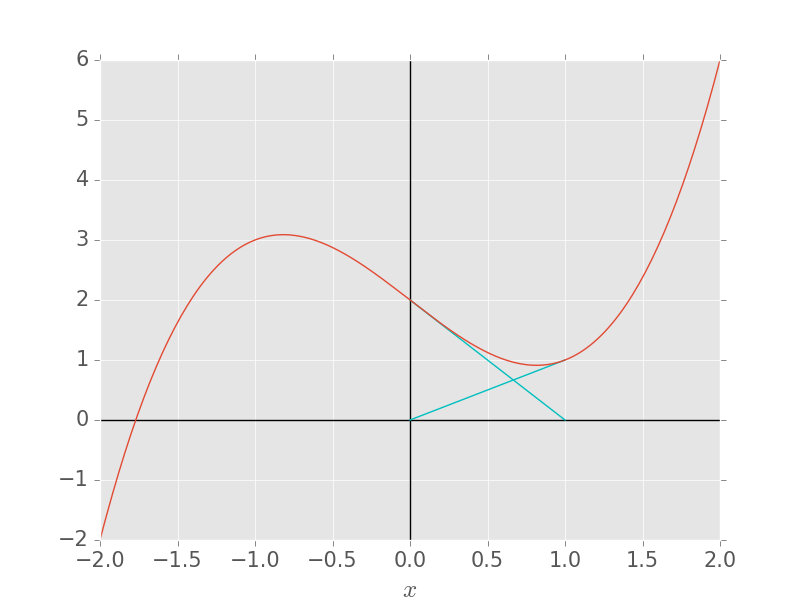
\includegraphics[width=0.7\linewidth,height=\textheight,keepaspectratio]{im/newton_fail1.png}
\end{center}

Other starting values, e.g.~\(x_0=-0.5\) can also be sucked into this
infinite loop! The correct answer is obtained for \(x_0=-1.0\).

\end{fbxSimple}

\begin{tcolorbox}[enhanced jigsaw, bottomrule=.15mm, colbacktitle=quarto-callout-note-color!10!white, breakable, arc=.35mm, coltitle=black, colback=white, bottomtitle=1mm, opacityback=0, title=\textcolor{quarto-callout-note-color}{\faInfo}\hspace{0.5em}{Note}, titlerule=0mm, toptitle=1mm, opacitybacktitle=0.6, colframe=quarto-callout-note-color-frame, leftrule=.75mm, rightrule=.15mm, left=2mm, toprule=.15mm]

The sensitivity of Newton's method to the choice of \(x_0\) is
beautifully illustrated by applying it to a \textbf{complex} function
such as \(f(z) = z^3 - 1\). The following plot colours points \(z_0\) in
the complex plane according to which root they converge to (\(1\),
\(e^{2\pi i/3}\), or \(e^{-2\pi i/3}\)):

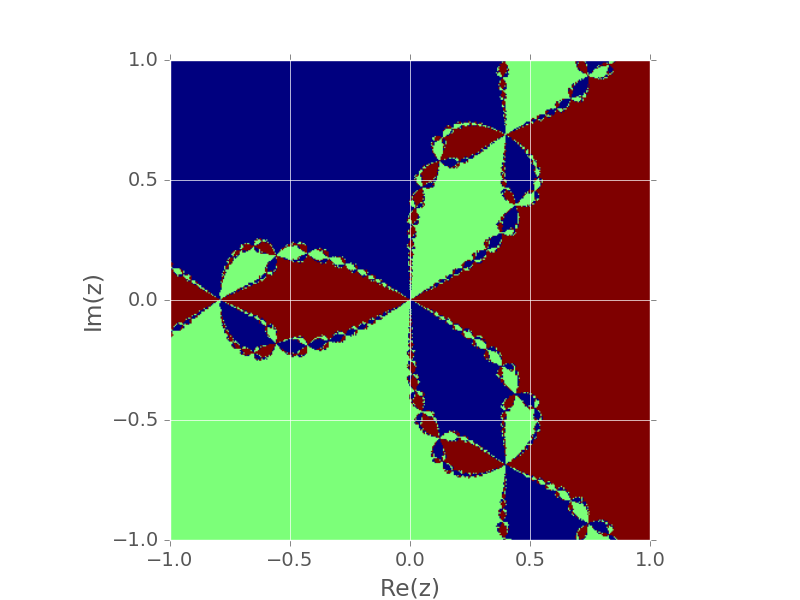
\includegraphics[width=0.8\linewidth,height=\textheight,keepaspectratio]{im/newton_basins.png}

The boundaries of these \textbf{basins of attraction} are fractal.

\end{tcolorbox}

\subsection{Newton's method for
systems}\label{newtons-method-for-systems}

Newton's method generalizes to higher-dimensional problems where we want
to find \(\mathbf{x}\in\mathbb{R}^m\) that satisfies
\(\mathbf{f}(\mathbf{x})=0\) for some function
\(\mathbf{f}:\mathbb{R}^m\to\mathbb{R}^m\).

To see how it works, take \(m=2\) so that \(\mathbf{x}=(x_1,x_2)^\top\)
and \(\mathbf{f}=[f_1(\mathbf{x}),f_2(\mathbf{x})]^\top\). Taking the
linear terms in Taylor's theorem for two variables gives \[
\begin{aligned}
0 &\approx f_1(\mathbf{x}_{k+1}) \approx f_1(\mathbf{x}_k) + \left.\frac{\partial f_1}{\partial x_1}\right|_{\mathbf{x}_k}(x_{1,k+1} - x_{1,k}) + \left.\frac{\partial f_1}{\partial x_2}\right|_{\mathbf{x}_k}(x_{2,k+1} - x_{2,k}),\\
0 &\approx f_2(\mathbf{x}_{k+1}) \approx f_2(\mathbf{x}_k) + \left.\frac{\partial f_2}{\partial x_1}\right|_{\mathbf{x}_k}(x_{1,k+1} - x_{1,k}) + \left.\frac{\partial f_2}{\partial x_2}\right|_{\mathbf{x}_k}(x_{2,k+1} - x_{2,k}).
\end{aligned}
\]

In matrix form, we can write \[
\begin{pmatrix}
0\\
0
\end{pmatrix}
=
\begin{pmatrix}
f_1(\mathbf{x}_k)\\
f_2(\mathbf{x}_k)
\end{pmatrix}
+
\begin{pmatrix}
\frac{\partial f_1}{\partial x_1}(\mathbf{x}_k) & \frac{\partial f_1}{\partial x_2}(\mathbf{x}_k)\\
\frac{\partial f_2}{\partial x_1}(\mathbf{x}_k) & \frac{\partial f_2}{\partial x_2}(\mathbf{x}_k)
\end{pmatrix}
\begin{pmatrix}
x_{1,k+1} - x_{1,k}\\
x_{2,k+1} - x_{2,k}
\end{pmatrix}.
\]

The matrix of partial derivatives is called the \textbf{Jacobian matrix}
\(J(\mathbf{x}_k)\), so (for any \(m\)) we have \[
\mathbf{0} = \mathbf{f}(\mathbf{x}_k) + J(\mathbf{x}_k)(\mathbf{x}_{k+1} - \mathbf{x}_{k}).
\]

To derive Newton's method, we rearrange this equation for
\(\mathbf{x}_{k+1}\), \[
J(\mathbf{x}_k)(\mathbf{x}_{k+1}-\mathbf{x}_k) = -\mathbf{f}(\mathbf{x}_k) \quad \implies \quad \mathbf{x}_{k+1} = \mathbf{x}_k - J^{-1}(\mathbf{x}_k)\mathbf{f}(\mathbf{x}_k).
\] So to apply the method, we need the inverse of \(J\).

\begin{tcolorbox}[enhanced jigsaw, bottomrule=.15mm, colbacktitle=quarto-callout-note-color!10!white, breakable, arc=.35mm, coltitle=black, colback=white, bottomtitle=1mm, opacityback=0, title=\textcolor{quarto-callout-note-color}{\faInfo}\hspace{0.5em}{Note}, titlerule=0mm, toptitle=1mm, opacitybacktitle=0.6, colframe=quarto-callout-note-color-frame, leftrule=.75mm, rightrule=.15mm, left=2mm, toprule=.15mm]

If \(m=1\), then \(J(x_k) = \frac{\partial f}{\partial x}(x_k)\), and
\(J^{-1}=1/J\), so this reduces to the scalar Newton's method.

\end{tcolorbox}

\phantomsection\label{apply-newtons-method-to-the-simultaneous-equations-xy---y3---1-0-and-x2y-y--50-with-starting-values-x_02-y_03.}
\begin{fbxSimple}{eg}{Example 2.26: }{Apply Newton’s method to the simultaneous equations \(xy - y^3 - 1 = 0\) and \(x^2y + y -5=0\), with starting values \(x_0=2\), \(y_0=3\).}
\phantomsection\label{apply-newtons-method-to-the-simultaneous-equations-xy---y3---1-0-and-x2y-y--50-with-starting-values-x_02-y_03.}
The Jacobian matrix is \[
J(x,y) = \begin{pmatrix}
y & x-3y^2\\
2xy & x^2 + 1
\end{pmatrix},
\] and hence its inverse is given by \[
J^{-1}(x,y) = \frac{1}{y(x^2+1)-2xy(x-3y^2)}\begin{pmatrix}
x^2 + 1 & 3y^2-x\\
-2xy & y
\end{pmatrix}.
\]

The first iteration of Newton's method gives \[
\begin{pmatrix}
x_1\\
y_1
\end{pmatrix}
= \begin{pmatrix}
2\\
3
\end{pmatrix}
- \frac{1}{3(5)-12(2-27)}
\begin{pmatrix}
5 & 25\\
-12 & 3
\end{pmatrix}
\begin{pmatrix}
-22\\
10
\end{pmatrix}
= \begin{pmatrix}
1.55555556\\
2.06666667
\end{pmatrix}.
\]

Subsequent iterations give \[
\begin{pmatrix}
x_2\\
y_2
\end{pmatrix}
=
\begin{pmatrix}
1.54720541\\
1.47779333
\end{pmatrix}, \, 
\begin{pmatrix}
x_3\\
y_3
\end{pmatrix}
=
\begin{pmatrix}
1.78053503\\
1.15886481
\end{pmatrix},
\] and \[
\begin{pmatrix}
x_4\\
y_4
\end{pmatrix}
=
\begin{pmatrix}
1.952843\\
1.02844269
\end{pmatrix}, \\ 
\begin{pmatrix}
x_5\\
y_5
\end{pmatrix}
=
\begin{pmatrix}
1.99776297\\
1.00124041
\end{pmatrix}, 
\]

so the method is converging accurately to the root \(x_*=2\), \(y_*=1\),
shown in the following plot:

\begin{center}
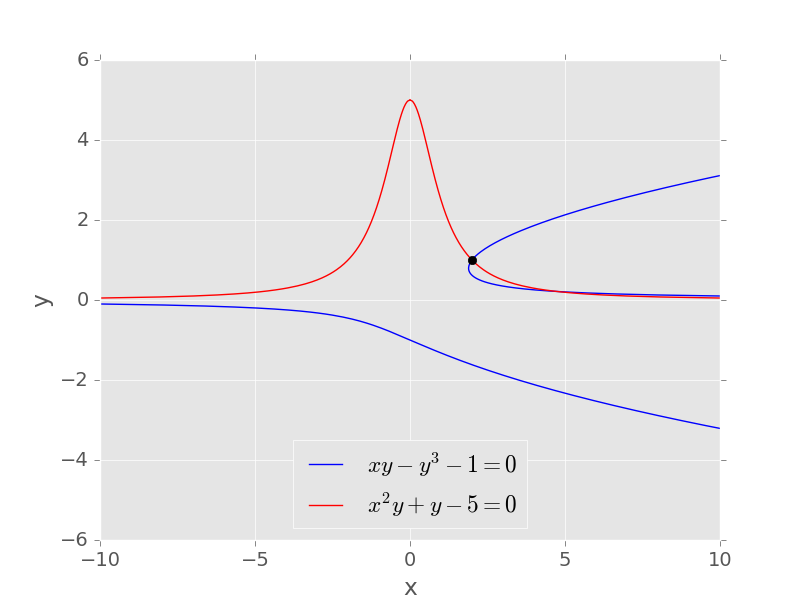
\includegraphics[width=0.7\linewidth,height=\textheight,keepaspectratio]{im/newton2d.png}
\end{center}

\end{fbxSimple}

By generalising the scalar analysis (beyond the scope of this course),
it can be shown that the convergence is quadratic for \(\mathbf{x}_0\)
sufficiently close to \(\mathbf{x}_*\), provided that
\(J(\mathbf{x}_*)\) is non-singular (i.e.,
\(\det[J(\mathbf{x}_*)]\neq 0\)).

\begin{tcolorbox}[enhanced jigsaw, bottomrule=.15mm, colbacktitle=quarto-callout-note-color!10!white, breakable, arc=.35mm, coltitle=black, colback=white, bottomtitle=1mm, opacityback=0, title=\textcolor{quarto-callout-note-color}{\faInfo}\hspace{0.5em}{Note}, titlerule=0mm, toptitle=1mm, opacitybacktitle=0.6, colframe=quarto-callout-note-color-frame, leftrule=.75mm, rightrule=.15mm, left=2mm, toprule=.15mm]

In general, finding a good starting point in more than one dimension is
difficult, particularly because interval bisection is not available.
Algorithms that try to mimic bisection in higher dimensions are
available, proceeding by a `grid search' approach.

\end{tcolorbox}

\subsection{Quasi-Newton methods}\label{quasi-newton-methods}

A drawback of Newton's method is that the derivative \(f'(x_k)\) must be
computed at each iteration. This may be expensive to compute, or may not
be available as a formula. For example, the function \(f\) might be the
right-hand side of some complex partial differential equation, and hence
both difficult to differentiate and very high dimensional!

Instead we can use a \textbf{quasi-Newton method} \[
x_{k+1} = x_k - \frac{f(x_k)}{g_k},
\] where \(g_k\) is some easily-computed approximation to \(f'(x_k)\).

\phantomsection\label{eg-2.27}
\begin{fbxSimple}{eg}{Example 2.27: }{Steffensen's method}
\phantomsection\label{eg-2.27}
\[
g_k = \frac{f\big(f(x_k) + x_k\big) - f(x_k)}{f(x_k)}.
\] This has the form \(\frac{1}{h}\big(f(x_k+h) - f(x_k)\big)\) with
\(h=f(x_k)\).

\end{fbxSimple}

Steffensen's method requires two function evaluations per iteration. But
once the iteration has started, we already have two nearby points
\(x_{k-1}\), \(x_k\), so we could approximate \(f'(x_k)\) by a backward
difference \[
g_k = \frac{f(x_k) - f(x_{k-1})}{x_k - x_{k-1}} \quad \implies \quad x_{k+1} = x_k - \frac{f(x_k)(x_k - x_{k-1})}{f(x_k) - f(x_{k-1})}.
\] This is called the \textbf{secant method}, and requires only one
function evaluation per iteration (once underway). The name comes from
its graphical interpretation:

\begin{center}
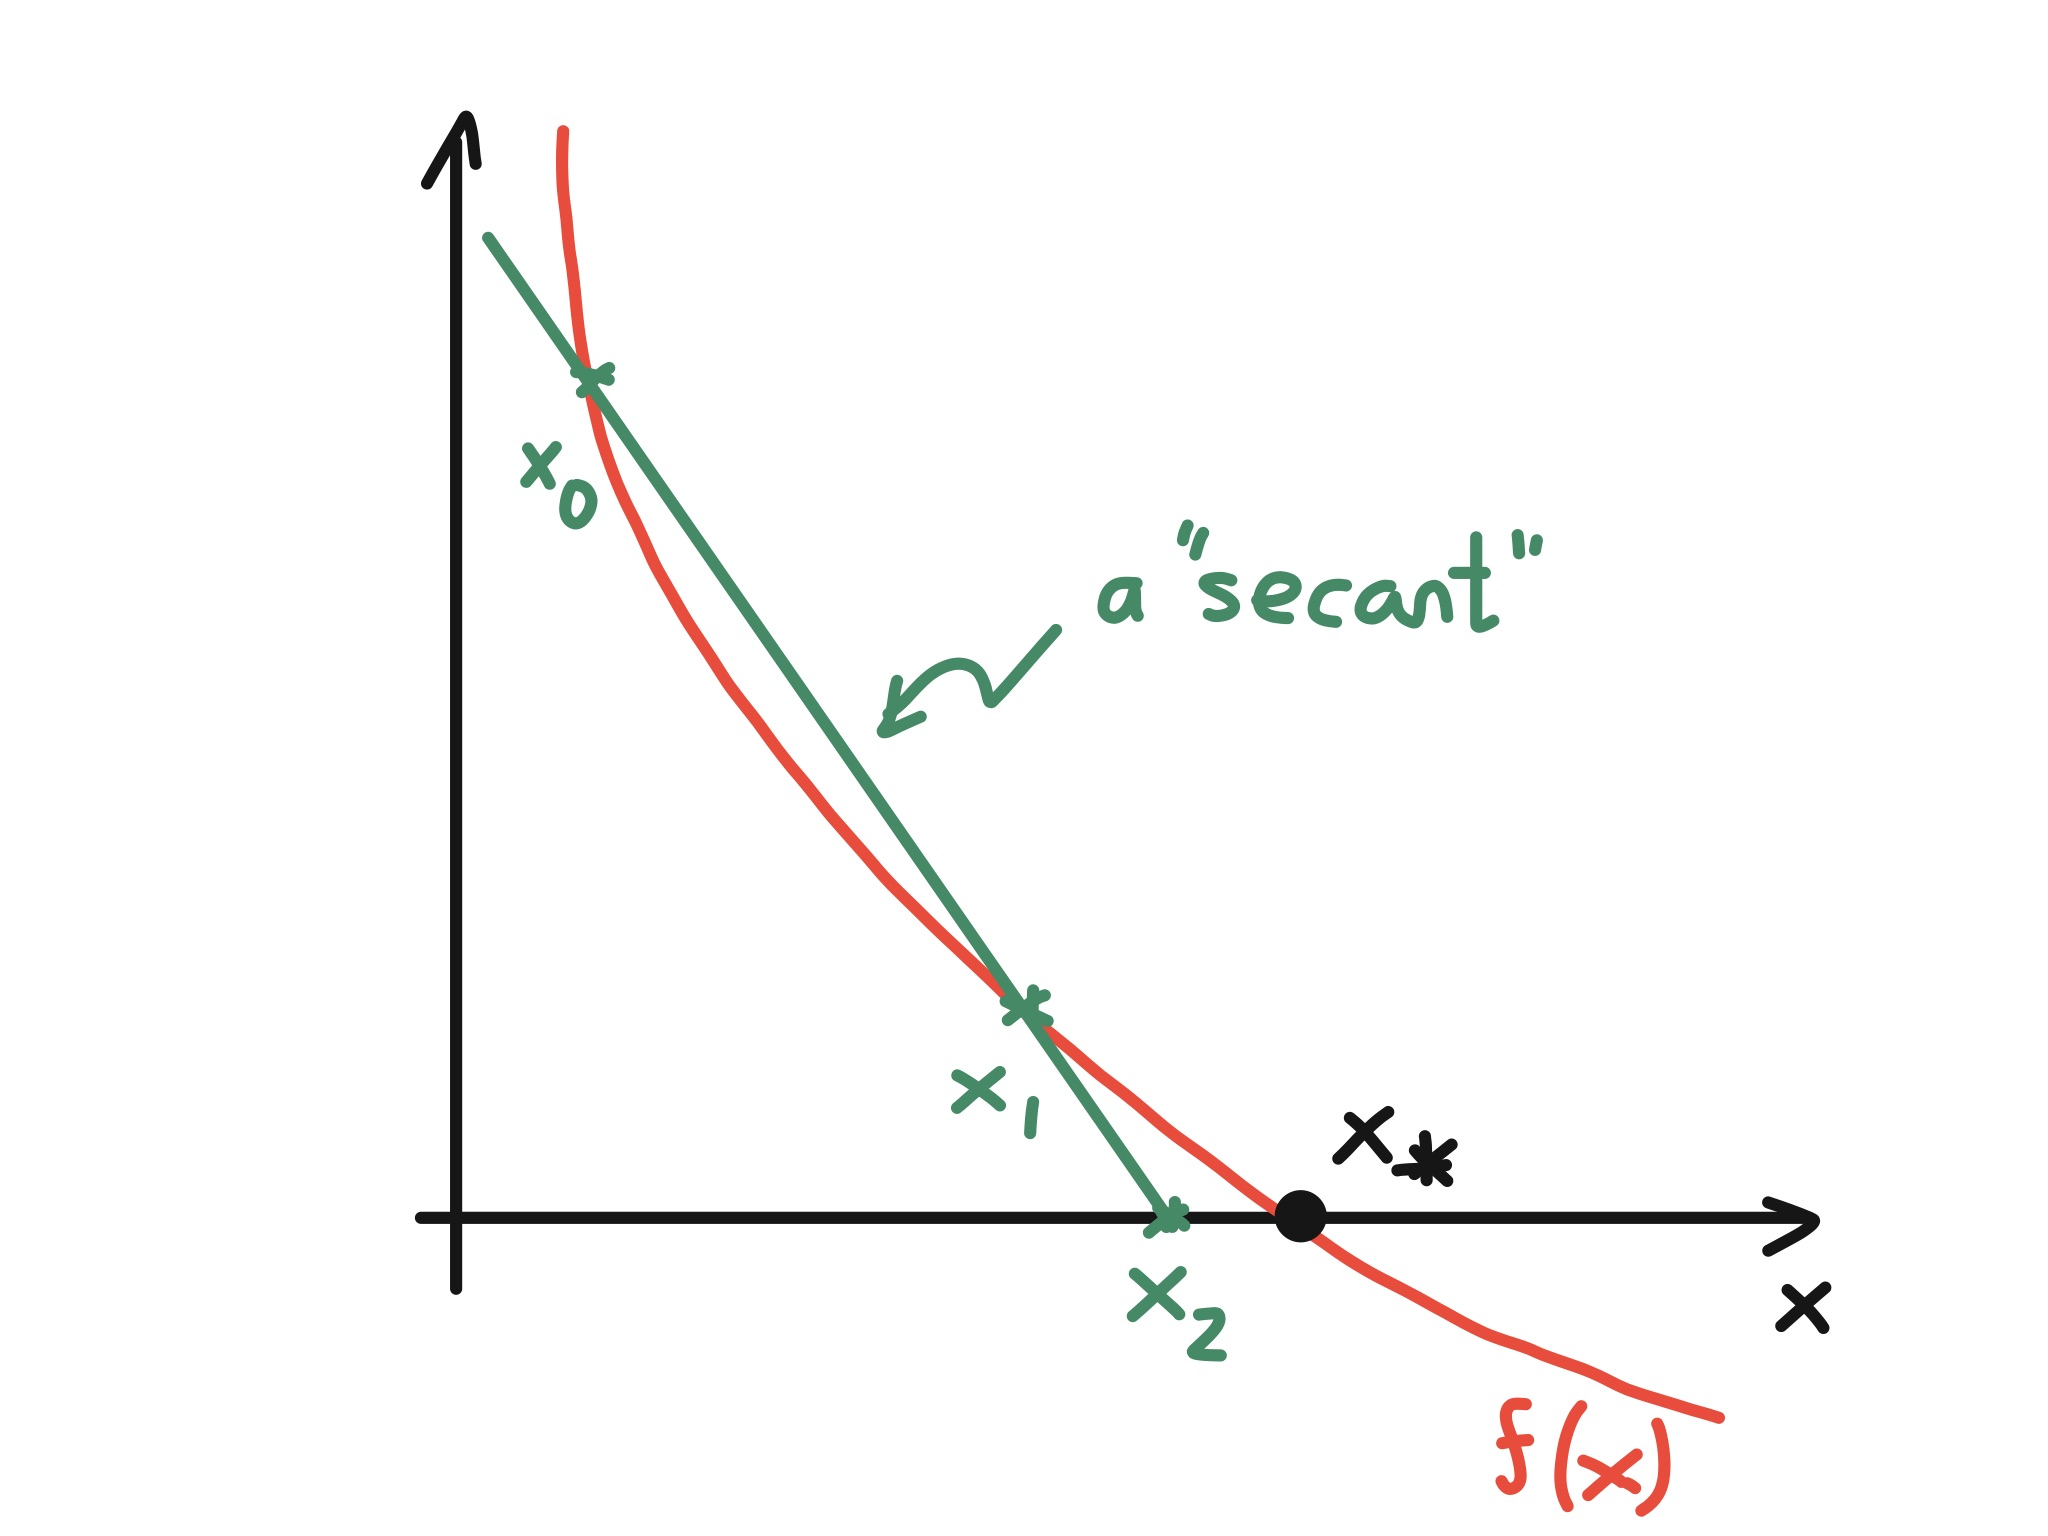
\includegraphics[width=0.7\linewidth,height=\textheight,keepaspectratio]{im/secant.jpg}
\end{center}

\begin{tcolorbox}[enhanced jigsaw, bottomrule=.15mm, colbacktitle=quarto-callout-note-color!10!white, breakable, arc=.35mm, coltitle=black, colback=white, bottomtitle=1mm, opacityback=0, title=\textcolor{quarto-callout-note-color}{\faInfo}\hspace{0.5em}{Note}, titlerule=0mm, toptitle=1mm, opacitybacktitle=0.6, colframe=quarto-callout-note-color-frame, leftrule=.75mm, rightrule=.15mm, left=2mm, toprule=.15mm]

The secant method was introduced by Newton.

\end{tcolorbox}

\phantomsection\label{fxtfrac1x---0.5.-1}
\begin{fbxSimple}{eg}{Example 2.28: }{\(f(x)=\tfrac1x - 0.5\).}
\phantomsection\label{fxtfrac1x---0.5.-1}
Now we need two starting values, so take \(x_0=0.25\), \(x_1=0.5\). The
secant method gives:

\begin{longtable}[]{@{}lll@{}}
\toprule\noalign{}
\(k\) & \(x_k\) & \(|x_* - x_k|/|x_* - x_{k-1}|\) \\
\midrule\noalign{}
\endhead
\bottomrule\noalign{}
\endlastfoot
2 & 0.6875 & 0.75 \\
3 & 1.01562 & 0.75 \\
4 & 1.354 & 0.65625 \\
5 & 1.68205 & 0.492188 \\
6 & 1.8973 & 0.322998 \\
7 & 1.98367 & 0.158976 \\
8 & 1.99916 & 0.0513488 \\
\end{longtable}

Convergence to \(\epsilon_{\rm M}\) is achieved in 12 iterations. Notice
that the error ratio is decreasing, so the convergence is superlinear.

\end{fbxSimple}

The secant method is a \textbf{two-point method} since
\(x_{k+1} = g(x_{k-1},x_k)\). So theorems about single-point fixed-point
iterations do not apply.

In general, one can have \textbf{multipoint methods} based on
higher-order interpolation.

\phantomsection\label{theorem-2.12}
\begin{fbxSimple}{theorem}{Theorem 2.12}{}
\phantomsection\label{theorem-2.12}
If \(f'(x_*)\neq 0\) then the secant method converges for \(x_0\),
\(x_1\) sufficiently close to \(x_*\), and the order of convergence is
\((1+\sqrt{5})/2 = 1.618\ldots\).

\end{fbxSimple}

\begin{tcolorbox}[enhanced jigsaw, bottomrule=.15mm, colbacktitle=quarto-callout-note-color!10!white, breakable, arc=.35mm, coltitle=black, colback=white, bottomtitle=1mm, opacityback=0, title=\textcolor{quarto-callout-note-color}{\faInfo}\hspace{0.5em}{Note}, titlerule=0mm, toptitle=1mm, opacitybacktitle=0.6, colframe=quarto-callout-note-color-frame, leftrule=.75mm, rightrule=.15mm, left=2mm, toprule=.15mm]

This illustrates that orders of convergence need not be integers, and is
also an appearance of the \textbf{golden ratio}.

\end{tcolorbox}

\textbf{Proof:}\\
To simplify the notation, denote the truncation error by \[
\varepsilon_k := x_* - x_k. 
\] Expanding in Taylor series around \(x_*\), and using \(f(x_*)=0\),
gives \[
\begin{aligned}
f(x_{k-1}) &= -f'(x_*)\varepsilon_{k-1} + \frac{f''(x_*)}{2}\varepsilon_{k-1}^2 + {\cal O}(\varepsilon_{k-1}^3),\\
f(x_{k}) &= -f'(x_*)\varepsilon_{k} + \frac{f''(x_*)}{2}\varepsilon_{k}^2 + {\cal O}(\varepsilon_{k}^3).
\end{aligned}
\] So using the secant formula above we get \[
\begin{aligned}
\varepsilon_{k+1} &= \varepsilon_k - (\varepsilon_{k}-\varepsilon_{k-1})\frac{-f'(x_*)\varepsilon_{k} + \frac{f''(x_*)}{2}\varepsilon_{k}^2 + {\cal O}(\varepsilon_{k}^3)}{-f'(x_*)(\varepsilon_{k}-\varepsilon_{k-1})+ \frac{f''(x_*)}{2}(\varepsilon_{k}^2 - \varepsilon_{k-1}^2) + {\cal O}(\varepsilon_{k-1}^3)}\\
&= \varepsilon_k - \frac{ -f'(x_*)\varepsilon_{k} + \frac{f''(x_*)}{2}\varepsilon_{k}^2 + {\cal O}(\varepsilon_{k}^3)}{-f'(x_*) + \frac{f''(x_*)}{2}(\varepsilon_k + \varepsilon_{k-1}) + {\cal O}(\varepsilon_{k-1}^2)}\\
&= \varepsilon_k + \frac{-\varepsilon_k + \tfrac12\varepsilon_k^2f''(x_*)/f'(x_*) + {\cal O}(\varepsilon_k^3)}{1 - \tfrac12(\varepsilon_k + \varepsilon_{k-1})f''(x_*)/f'(x_*) + {\cal O}(\varepsilon_{k-1}^2)}\\
&= \varepsilon_k + \left(-\varepsilon_k + \frac{f''(x_*)}{2f'(x_*)}\varepsilon_k^2 + {\cal O}(\varepsilon_k^3) \right)\left(1 + (\varepsilon_k + \varepsilon_{k-1})\frac{f''(x_*)}{2f'(x_*)} + {\cal O}(\varepsilon_{k-1}^2) \right)\\
&= \varepsilon_k - \varepsilon_k + \frac{f''(x_*)}{2f'(x_*)}\varepsilon_k^2 - \frac{f''(x_*)}{2f'(x_*)}\varepsilon_k(\varepsilon_k + \varepsilon_{k-1}) + {\cal O}(\varepsilon_{k-1}^3)\\
&= -\frac{f''(x_*)}{2f'(x_*)}\varepsilon_k\varepsilon_{k-1} + {\cal O}(\varepsilon_{k-1}^3).
\end{aligned}
\] This is similar to the corresponding formula for Newton's method,
where we have \[
\varepsilon_{k+1} = -\frac{f''(x_*)}{2f'(x_*)}\varepsilon_k^2 + {\cal O}(\varepsilon_k^3).
\] The above tells us that the error for the secant method tends to zero
faster than linearly, but not quadratically (because
\(\varepsilon_{k-1} > \varepsilon_k\)).

To find the order of convergence, note that
\(\varepsilon_{k+1}\sim \varepsilon_k\varepsilon_{k-1}\) suggests a
power-law relation of the form \[
|\varepsilon_k| = |\varepsilon_{k-1}|^\alpha\left|\frac{f''(x_*)}{2f'(x_*)}\right|^\beta \quad \implies \quad |\varepsilon_{k-1}| = |\varepsilon_k|^{1/\alpha}\left|\frac{f''(x_*)}{2f'(x_*)}\right|^{-\beta/\alpha}.
\] Putting this in both sides of the previous equation gives \[
|\varepsilon_{k}|^\alpha\left|\frac{f''(x_*)}{2f'(x_*)}\right|^\beta = |\varepsilon_k|^{(1+\alpha)/\alpha}\left|\frac{f''(x_*)}{2f'(x_*)}\right|^{(\alpha-\beta)/\alpha}.
\] Equating powers gives \[
\alpha = \frac{1+\alpha}{\alpha} \quad \implies \alpha = \frac{1 + \sqrt{5}}{2}, \quad \beta = \frac{\alpha - \beta}{\alpha} \quad \implies \beta = \frac{\alpha}{\alpha + 1} = \frac{1}{\alpha}.
\] It follows that \[
\lim_{k\to\infty}\frac{|x_* - x_{k+1}|}{|x_* - x_k|^\alpha} = \lim_{k\to\infty}\frac{|\varepsilon_{k+1}|}{|\varepsilon_k|^\alpha} = \left|\frac{f''(x_*)}{2f'(x_*)}\right|^{1/\alpha},
\] so the secant method has order of convergence \(\alpha\).

\section*{Knowledge checklist}\label{knowledge-checklist-1}
\addcontentsline{toc}{section}{Knowledge checklist}

\markright{Knowledge checklist}

\textbf{Key topics:}

\begin{enumerate}
\def\labelenumi{\arabic{enumi}.}
\item
  Polynomial interpolation, including the Lagrange and Newton
  divided-difference forms of polynomial interpolation.
\item
  Interpolation error estimates, truncation error, and the significance
  of node placement (e.g.~the Runge phenomenon).
\item
  Numerical rootfinding methods, including interval bisection and fixed
  point iteration, with discussion of existence, uniqueness, and orders
  of convergence (linear, superlinear).
\end{enumerate}

\textbf{Key skills:}

\begin{itemize}
\item
  Constructing and analyzing polynomial interpolants for a given data
  set and function, using Taylor, Lagrange, and Newton methods.
\item
  Estimating approximation errors and choosing optimal interpolation
  nodes to improve numerical stability and convergence.
\item
  Implementing and evaluating iterative algorithms for solving nonlinear
  equations, including measuring and understanding convergence rates.
\end{itemize}

\bookmarksetup{startatroot}

\chapter{Linear Algebra}\label{linear-algebra}

\section{Systems of Linear Equations}\label{s-lin}

The central goal of this chapter is to answer the following seemingly
straightforward question:

\begin{quote}
\emph{How do we solve a linear system numerically?}
\end{quote}

Linear systems of the form \[
\begin{aligned}
a_{11}x_1 &+ a_{12}x_2 + \ldots + a_{1n}x_n = b_1,\\
a_{21}x_1 &+ a_{22}x_2 + \ldots + a_{2n}x_n = b_2,\\
\vdots    &\qquad\vdots\qquad\qquad\vdots\\
a_{n1}x_1 &+ a_{n2}x_2 + \ldots + a_{nn}x_n = b_n
\end{aligned}
\] occur in many applications (often with very large \(n\)). It is
convenient to express this in matrix form: \[
A\mathbf{x} = \mathbf{b},
\] where \(A\) is an \(n\times n\) square matrix with elements
\(a_{ij}\), and \(\mathbf{x}\), \(\mathbf{b}\) are \(n\times 1\)
vectors.

We will need some basic facts from linear algebra:

\begin{enumerate}
\def\labelenumi{\arabic{enumi}.}
\item
  \(A^\top\) is the \textbf{transpose} of \(A\), so
  \((a^\top)_{ij} = a_{ji}\).
\item
  \(A\) is \textbf{symmetric} if \(A=A^\top\).
\item
  \(A\) is \textbf{non-singular} iff there exists a solution
  \(\mathbf{x}\in\mathbb{R}^n\) for every \(\mathbf{b}\in\mathbb{R}^n\).
\item
  \(A\) is non-singular iff \(\det(A)\neq 0\).
\item
  \(A\) is non-singular iff there exists a unique \textbf{inverse}
  \(A^{-1}\) such that \(AA^{-1}=A^{-1}A = I\).
\end{enumerate}

It follows from fact 5 above that \(A\mathbf{x} = \mathbf{b}\) has a
unique solution iff \(A\) is non-singular, given by
\(\mathbf{x} = A^{-1}\mathbf{b}\).

In this chapter, we will see how to solve \(A\mathbf{x} = \mathbf{b}\)
both \textbf{efficiently} and \textbf{accurately}.

Although this seems like a conceptually easy problem (just use Gaussian
elimination!), it is actually a hard one when \(n\) gets large.
Nowadays, linear systems with \(n=1\) million arise routinely in
computational problems. And even for small \(n\) there are some
potential pitfalls, as we will see.

\begin{tcolorbox}[enhanced jigsaw, bottomrule=.15mm, colbacktitle=quarto-callout-note-color!10!white, breakable, arc=.35mm, coltitle=black, colback=white, bottomtitle=1mm, opacityback=0, title=\textcolor{quarto-callout-note-color}{\faInfo}\hspace{0.5em}{Note}, titlerule=0mm, toptitle=1mm, opacitybacktitle=0.6, colframe=quarto-callout-note-color-frame, leftrule=.75mm, rightrule=.15mm, left=2mm, toprule=.15mm]

If \(A\) is instead rectangular (\(m\times n\)), then there are
different numbers of equations and unknowns, and we do not expect a
unique solution. Nevertheless, we can still look for an approximate
solution in this case and there are methods for this problem in the
course reading list.

\end{tcolorbox}

Many algorithms are based on the idea of rewriting
\(A\mathbf{x} = \mathbf{b}\) in a form where the matrix is easier to
invert. Easiest to invert are diagonal matrices, followed by orthogonal
matrices (where \(A^{-1}=A^\top\)). However, the most common method for
solving \(A\mathbf{x} = \mathbf{b}\) transforms the system to
\emph{triangular} form.

\section{Triangular systems}\label{triangular-systems}

If the matrix \(A\) is triangular, then \(A\mathbf{x} = \mathbf{b}\) is
straightforward to solve.

A matrix \(L\) is called \textbf{lower triangular} if all entries above
the diagonal are zero: \[
L = \begin{pmatrix}
l_{11} & 0 & \cdots & 0\\
l_{21} & l_{22} & \ddots & \vdots\\
\vdots & &\ddots & 0\\
l_{n1} & \cdots & \cdots & l_{nn}
\end{pmatrix}.
\] The determinant is just \[
\det(L) = l_{11}l_{22}\cdots l_{nn},
\] so the matrix will be non-singular iff all of the diagonal elements
are non-zero.

\phantomsection\label{solve-lmathbfx-mathbfb-for-n4.}
\begin{fbxSimple}{eg}{Example 3.1: }{Solve \(L\mathbf{x} = \mathbf{b}\) for \(n=4\).}
\phantomsection\label{solve-lmathbfx-mathbfb-for-n4.}
The system is \[
\begin{pmatrix}
l_{11} & 0 & 0 & 0\\
l_{21} & l_{22} & 0 & 0\\
l_{31} & l_{32} & l_{33} & 0\\
l_{41} & l_{42} & l_{43} & l_{44}
\end{pmatrix}
\begin{pmatrix}
x_1\\ x_2\\ x_3\\ x_4
\end{pmatrix}
=
\begin{pmatrix}
b_1\\ b_2\\ b_3\\ b_4
\end{pmatrix}
\] which is equivalent to \[
\begin{aligned}
l_{11}x_1 &= b_1,\\
l_{21}x_1 + l_{22}x_2 &= b_2,\\
l_{31}x_1 + l_{32}x_2 + l_{33}x_3 &= b_3,\\
l_{41}x_1 + l_{42}x_2 + l_{43}x_3 + l_{44}x_4 &= b_4.
\end{aligned}
\] We can just solve step-by-step: \[
x_1 = \frac{b_1}{l_{11}}, \,\, x_2 = \frac{b_2 - l_{21}x_1}{l_{22}},
\]
\[x_3 = \frac{b_3 - l_{31}x_1 - l_{32}x_2}{l_{33}}, \,\, x_4 = \frac{b_4 - l_{41}x_1 - l_{42}x_2 - l_{43}x_3}{l_{44}}.
\] This is fine since we know that \(l_{11}\), \(l_{22}\), \(l_{33}\),
\(l_{44}\) are all non-zero when a solution exists.

\end{fbxSimple}

In general, any lower triangular system \(L\mathbf{x}=\mathbf{b}\) can
be solved by \textbf{forward substitution} \[
x_j = \frac{b_j - \sum_{k=1}^{j-1}l_{jk}x_k}{l_{jj}}, \quad j=1,\ldots,n.
\]

Similarly, an \textbf{upper triangular} matrix \(U\) has the form \[
U = \begin{pmatrix}
u_{11} & u_{12} & \cdots & u_{1n}\\
0 & u_{22} & & \vdots\\
\vdots & \ddots & \ddots & \vdots\\
0 & \cdots & 0 & u_{nn}
\end{pmatrix},
\] and an upper-triangular system \(U\mathbf{x} = \mathbf{b}\) may be
solved by \textbf{backward substitution} \[
x_j = \frac{b_j - \sum_{k=j+1}^{n}u_{jk}x_k}{u_{jj}}, \quad j=n,\ldots,1.
\]

To estimate the computational cost of forward substitution, we can count
the number of floating-point operations (\(+\), \(-\), \(\times\),
\(\div\)).

\phantomsection\label{eg-3.2}
\begin{fbxSimple}{eg}{Example 3.2: }{Number of operations required for forward substitution.}
\phantomsection\label{eg-3.2}
Consider each \(x_j\). We have - \(j=1\): 1 division - \(j=2\): 1
division + {[}1 subtraction + 1 multiplication{]} - \(j=3\): 1 division
+ \(2\,\times\){[}1 subtraction + 1 multiplication{]} - \(\vdots\) -
\(j=n\): 1 division + \((n-1)\,\times\){[}1 subtraction + 1
multiplication{]}

So the total number of operations required is \[
\sum_{j=1}^n\Big(1 + 2(j-1)\Big) = 2\sum_{j=1}^nj - \sum_{j=1}^n1 = n(n+1) - n = n^2.
\]

\end{fbxSimple}

So solving a triangular system by forward (or backward) substitution
takes \(n^2\) operations. We may say that the \textbf{computational
complexity} of the algorithm is \(n^2\).

\begin{tcolorbox}[enhanced jigsaw, bottomrule=.15mm, colbacktitle=quarto-callout-note-color!10!white, breakable, arc=.35mm, coltitle=black, colback=white, bottomtitle=1mm, opacityback=0, title=\textcolor{quarto-callout-note-color}{\faInfo}\hspace{0.5em}{Note}, titlerule=0mm, toptitle=1mm, opacitybacktitle=0.6, colframe=quarto-callout-note-color-frame, leftrule=.75mm, rightrule=.15mm, left=2mm, toprule=.15mm]

In practice, this is only a rough estimate of the computational cost,
because reading from and writing to the computer's memory also take
time. This can be estimated given a ``memory model'', but this depends
on the particular computer.

\end{tcolorbox}

\section{Gaussian elimination}\label{gaussian-elimination}

If our matrix \(A\) is not triangular, we can try to transform it to
triangular form. \textbf{Gaussian elimination} uses elementary row
operations to transform the system to upper triangular form
\(U\mathbf{x} = \mathbf{y}\).

Elementary row operations include swapping rows and adding multiples of
one row to another. They won't change the solution \(\mathbf{x}\), but
will change the matrix \(A\) and the right-hand side \(\mathbf{b}\).

\phantomsection\label{eg-3.3}
\begin{fbxSimple}{eg}{Example 3.3: }{Transform to upper triangular form the system}
\phantomsection\label{eg-3.3}
\[
\begin{aligned}
x_1 + 2x_2 + x_3 &= 0,\\
x_1 - 2x_2 + 2x_3 &= 4,\\
2x_1 + 12x_2 - 2x_3 &= 4.
\end{aligned}
\] \[
A=\begin{pmatrix}
1 & 2 & 1\\
1 & -2 & 2\\
2 & 12 & -2
\end{pmatrix},
\quad
\mathbf{b}=\begin{pmatrix}
0\\ 4\\ 4
\end{pmatrix}.
\]

\textbf{Stage 1.} Subtract \(1\) times equation 1 from equation 2, and
\(2\) times equation 1 from equation 3, so as to eliminate \(x_1\) from
equations 2 and 3: \[
\begin{aligned}
x_1 + 2x_2 + x_3 &= 0,\\
-4x_2 + x_3 &= 4,\\
8x_2 - 4x_3 &= 4.
\end{aligned}
\] \[
A^{(2)}=\begin{pmatrix}
1 & 2 & 1\\
0 & -4 & 1\\
0 & 8 & -4
\end{pmatrix}
\quad
\mathbf{b}^{(2)}=\begin{pmatrix}
0\\ 4\\ 4
\end{pmatrix},
\quad m_{21}=1, \quad m_{31}=2.
\]

\textbf{Stage 2.} Subtract \(-2\) times equation 2 from equation 3, to
eliminate \(x_2\) from equation 3: \[
\begin{aligned}
x_1 + 2x_2 + x_3 &= 0,\\
-4x_2 + x_3 &= 4,\\
-2x_3 = 12.
\end{aligned}
\] \[
A^{(3)}=\begin{pmatrix}
1 & 2 & 1\\
0 & -4 & 1\\
0 & 0 & -2
\end{pmatrix}
\quad
\mathbf{b}^{(3)}=\begin{pmatrix}
0\\ 4\\ 12
\end{pmatrix},
\quad m_{32}=-2.
\]

Now the system is upper triangular, and back substitution gives
\(x_1=11\), \(x_2=-\tfrac{5}{2}\), \(x_3=-6\).

\end{fbxSimple}

We can write the general algorithm as follows.

\phantomsection\label{algorithm-3.1}
\begin{fbxSimple}{algorithm}{Algorithm 3.1: }{Gaussian elimination}
\phantomsection\label{algorithm-3.1}

Let \(A^{(1)}=A\) and \(\mathbf{b}^{(1)}=\mathbf{b}\). Then for each
\(k\) from 1 to \(n-1\), compute a new matrix \(A^{(k+1)}\) and
right-hand side \(\mathbf{b}^{(k+1)}\) by the following procedure:

\begin{enumerate}
\def\labelenumi{\arabic{enumi}.}
\tightlist
\item
  Define the row multipliers \[
  m_{ik} = \frac{a_{ik}^{(k)}}{a_{kk}^{(k)}}, \quad i=k+1,\ldots,n.
  \]
\item
  Use these to remove the unknown \(x_k\) from equations \(k+1\) to
  \(n\), leaving \[
  a_{ij}^{(k+1)} = a_{ij}^{(k)} - m_{ik}a_{kj}^{(k)}, \quad b_i^{(k+1)} = b_i^{(k)} - m_{ik}b_k^{(k)}, \quad i,j=k+1,\ldots,n.
  \] The final matrix \(A^{(n)}=U\) will then be upper triangular.
\end{enumerate}

\end{fbxSimple}

This procedure will work providing \(a_{kk}^{(k)}\neq 0\) for every
\(k\). (We will worry about this later.)

What about the computational cost of Gaussian elimination?

\phantomsection\label{number-of-operations-required-to-find-u.}
\begin{fbxSimple}{eg}{Example 3.4: }{Number of operations required to find \(U\).}
\phantomsection\label{number-of-operations-required-to-find-u.}
Computing \(A^{(k+1)}\) requires: - \(n-(k+1)+1 = n-k\) divisions to
compute \(m_{ik}\). - \((n-k)^2\) subtractions and the same number of
multiplications to compute \(a_{ij}^{(k+1)}\).

So in total \(A^{(k+1)}\) requires \(2(n-k)^2 + n-k\) operations.
Overall, we need to compute \(A^{(k+1)}\) for \(k=1,\ldots,n-1\), so the
total number of operations is \[
\begin{aligned}
N &= \sum_{k=1}^{n-1}\Big(2n^2 + n - (4n+1)k + 2k^2\Big) \\
  &= n(2n+1)\sum_{k=1}^{n-1}1 - (4n+1)\sum_{k=1}^{n-1}k + 2\sum_{k=1}^{n-1}k^2.
\end{aligned}
\] Recalling that \[
\sum_{k=1}^n k = \tfrac12n(n+1), \,\, \sum_{k=1}^n k^2 = \tfrac16n(n+1)(2n+1),
\] we find \[
\begin{aligned}
N &= n(2n+1)(n-1) - \tfrac12(4n+1)(n-1)n + \tfrac13(n-1)n(2n-1) \\
&= \tfrac23n^3 - \tfrac12n^2 - \tfrac16n.
\end{aligned}
\] So the number of operations required to find \(U\) is
\({\cal O}(n^3)\).

\end{fbxSimple}

It is known that \({\cal O}(n^3)\) is not optimal, and the best
theoretical algorithm known for inverting a matrix takes
\({\cal O}(n^{2.3728639})\) operations. However, algorithms achieving
this bound are highly impractical for most real-world uses due to
massive constant factors and implementation overhead. It remains an open
conjecture that there exists an \({\cal O}(n^{2+\epsilon})\) algorithm,
for \(\epsilon\) arbitrarily small.

\section{LU decomposition}\label{lu-decomposition}

In Gaussian elimination, both the final matrix \(U\) and the sequence of
row operations are determined solely by \(A\), and do not depend on
\(\mathbf{b}\). We will see that the sequence of row operations that
transforms \(A\) to \(U\) is equivalent to left-multiplying by a matrix
\(F\), so that \[
FA = U, \qquad U\mathbf{x} = F\mathbf{b}.
\] To see this, note that step \(k\) of Gaussian elimination can be
written in the form \[
A^{(k+1)} = F^{(k)}A^{(k)}, \quad \mathbf{b}^{(k+1)} = F^{(k)}\mathbf{b}^{(k)},
\] where \[
F^{(k)} := \begin{pmatrix}
1 & 0&\cdots & \cdots &\cdots&0\\
0 & \ddots & \ddots&&&\vdots \\
\vdots & \ddots& 1 &\ddots&&\vdots \\
\vdots & & -m_{k+1,k} & \ddots &\ddots&\vdots \\
\vdots & & \vdots & \ddots& \ddots &0\\
0& \cdots  & -m_{n,k} &\cdots&0&1
\end{pmatrix}.
\] Multiplying by \(F^{(k)}\) has the effect of subtracting \(m_{ik}\)
times row \(k\) from row \(i\), for \(i=k+1,\ldots,n\).

\begin{tcolorbox}[enhanced jigsaw, bottomrule=.15mm, colbacktitle=quarto-callout-note-color!10!white, breakable, arc=.35mm, coltitle=black, colback=white, bottomtitle=1mm, opacityback=0, title=\textcolor{quarto-callout-note-color}{\faInfo}\hspace{0.5em}{Note}, titlerule=0mm, toptitle=1mm, opacitybacktitle=0.6, colframe=quarto-callout-note-color-frame, leftrule=.75mm, rightrule=.15mm, left=2mm, toprule=.15mm]

A matrix with this structure (the identity except for a single column
below the diagonal) is called a \textbf{Frobenius matrix}.

\end{tcolorbox}

\phantomsection\label{eg-3.5}
\begin{fbxSimple}{eg}{Example 3.5}{}
\phantomsection\label{eg-3.5}
You can check in the earlier example that \[
F^{(1)}A=\begin{pmatrix}
1 & 0 & 0\\
-1 & 1 & 0\\
-2 & 0 & 1
\end{pmatrix}
\begin{pmatrix}
1 & 2 & 1\\
1 & -2 & 2\\
2 & 12 & -2
\end{pmatrix}
=
\begin{pmatrix}
1 & 2 & 1\\
0 & -4 & 1\\
0 & 8 & -4
\end{pmatrix} = A^{(2)},
\] and \[
F^{(2)}A^{(2)}=
\begin{pmatrix}
1 & 0 & 0\\
0 & 1 & 0\\
0 & 2 & 1
\end{pmatrix}
\begin{pmatrix}
1 & 2 & 1\\
0 & -4 & 1\\
0 & 8 & -4
\end{pmatrix}
=
\begin{pmatrix}
1 & 2 & 1\\
0 & -4 & 1\\
0 & 0 & -2
\end{pmatrix} = A^{(3)}=U.
\]

\end{fbxSimple}

It follows that \[
U = A^{(n)} = F^{(n-1)}F^{(n-2)}\cdots F^{(1)}A.
\] Now the \(F^{(k)}\) are invertible, and the inverse is just given by
adding rows instead of subtracting: \[
(F^{(k)})^{-1} = \begin{pmatrix}
1 & 0&\cdots & \cdots &\cdots&0\\
0 & \ddots & \ddots&&&\vdots \\
\vdots & \ddots& 1 &\ddots&&\vdots \\
\vdots & & m_{k+1,k} & \ddots &\ddots&\vdots \\
\vdots & & \vdots & \ddots& \ddots &0\\
0& \cdots  & m_{n,k} &\cdots&0&1
\end{pmatrix}.
\] So we could write \[
A = (F^{(1)})^{-1}(F^{(2)})^{-1}\cdots (F^{(n-1)})^{-1}U.
\] Since the successive operations don't ``interfere'' with each other,
we can write \[
  (F^{(1)})^{-1}(F^{(2)})^{-1}\cdots (F^{(n-1)})^{-1} =  \begin{pmatrix}
1 & 0& \cdots&\cdots&\cdots&0\\
m_{2,1} & 1 &\ddots&&&\vdots\\
m_{3,1} & m_{3,2} & 1&\ddots&&\vdots\\
m_{4,1} & m_{4,2} & m_{4,3}&\ddots&\ddots&\vdots\\
\vdots & \vdots&\vdots&&1&0\\
m_{n,1} & m_{n,2} & m_{n,3}&\cdots&m_{n,n-1} &1
\end{pmatrix} := L.
\] Thus we have established the following result.

\phantomsection\label{theorem-3.1}
\begin{fbxSimple}{theorem}{Theorem 3.1: }{LU decomposition}
\phantomsection\label{theorem-3.1}
Let \(U\) be the upper triangular matrix from Gaussian elimination of
\(A\) (without pivoting), and let \(L\) be the unit lower triangular
matrix above. Then \[
A = LU.
\]

\end{fbxSimple}

\begin{tcolorbox}[enhanced jigsaw, bottomrule=.15mm, colbacktitle=quarto-callout-note-color!10!white, breakable, arc=.35mm, coltitle=black, colback=white, bottomtitle=1mm, opacityback=0, title=\textcolor{quarto-callout-note-color}{\faInfo}\hspace{0.5em}{Note}, titlerule=0mm, toptitle=1mm, opacitybacktitle=0.6, colframe=quarto-callout-note-color-frame, leftrule=.75mm, rightrule=.15mm, left=2mm, toprule=.15mm]

\emph{Unit} lower triangular means that there are all 1's on the
diagonal.

\end{tcolorbox}

The theorem above says that Gaussian elimination is equivalent to
factorising \(A\) as the product of a lower triangular and an upper
triangular matrix. This is not at all obvious from the algorithm! The
decomposition is unique up to a scaling \(LD\), \(D^{-1}U\) for some
diagonal matrix \(D\).

The system \(A\mathbf{x}=\mathbf{b}\) becomes
\(LU\mathbf{x}=\mathbf{b}\), which we can readily solve by setting
\(U\mathbf{x}=\mathbf{y}\). We first solve \(L\mathbf{y}=\mathbf{b}\)
for \(\mathbf{y}\), then \(U\mathbf{x}=\mathbf{y}\) for \(\mathbf{x}\).
Both are triangular systems.

Moreover, if we want to solve several systems
\(A\mathbf{x} = \mathbf{b}\) with different \(\mathbf{b}\) but the same
matrix, we just need to compute \(L\) and \(U\) once. This saves time
because, although the initial \(LU\) factorisation takes
\({\cal O}(n^3)\) operations, the evaluation takes only
\({\cal O}(n^2)\).

\begin{tcolorbox}[enhanced jigsaw, bottomrule=.15mm, colbacktitle=quarto-callout-note-color!10!white, breakable, arc=.35mm, coltitle=black, colback=white, bottomtitle=1mm, opacityback=0, title=\textcolor{quarto-callout-note-color}{\faInfo}\hspace{0.5em}{Note}, titlerule=0mm, toptitle=1mm, opacitybacktitle=0.6, colframe=quarto-callout-note-color-frame, leftrule=.75mm, rightrule=.15mm, left=2mm, toprule=.15mm]

This matrix factorisation viewpoint dates only from the 1940s, and LU
decomposition was introduced by Alan Turing in a 1948 paper (\emph{Q. J.
Mechanics Appl. Mat.} \textbf{1}, 287). Other common factorisations used
in numerical linear algebra are \textbf{QR} (which we will see later)
and \emph{Cholesky}.

\end{tcolorbox}

\phantomsection\label{eg-3.6}
\begin{fbxSimple}{eg}{Example 3.6}{}
\phantomsection\label{eg-3.6}
Solve our earlier example by LU decomposition.

\[
\begin{pmatrix}
1 & 2 & 1\\
1 & -2 & 2\\
2 & 12 & -2
\end{pmatrix}
\begin{pmatrix}
x_1\\ x_2\\ x_3
\end{pmatrix}
=
\begin{pmatrix}
0\\ 4\\ 4
\end{pmatrix}.
\]

We apply Gaussian elimination as before, but ignore \(\mathbf{b}\) (for
now), leading to \[
U = \begin{pmatrix}
1 & 2 & 1\\
0 & -4 & 1\\
0 & 0 & -2
\end{pmatrix}.
\] As we apply the elimination, we record the multipliers so as to
construct the matrix \[
L = \begin{pmatrix}
1 & 0 & 0\\
1 & 1 & 0\\
2 & -2 & 1
\end{pmatrix}.
\] Thus we have the factorisation/decomposition \[
\begin{pmatrix}
1 & 2 & 1\\
1 & -2 & 2\\
2 & 12 & -2
\end{pmatrix} =
\begin{pmatrix}
1 & 0 & 0\\
1 & 1 & 0\\
2 & -2 & 1
\end{pmatrix}
\begin{pmatrix}
1 & 2 & 1\\
0 & -4 & 1\\
0 & 0 & -2
\end{pmatrix}.
\]

With the matrices \(L\) and \(U\), we can readily solve for any
right-hand side \(\mathbf{b}\). We illustrate for our particular
\(\mathbf{b}\). Firstly, solve \(L\mathbf{y}=\mathbf{b}\): \[
\begin{pmatrix}
1 & 0 & 0\\
1 & 1 & 0\\
2 & -2 & 1
\end{pmatrix}
\begin{pmatrix}
y_1\\y_2\\y_3
\end{pmatrix}
=
\begin{pmatrix}
0\\ 4\\ 4
\end{pmatrix}
\] \[
\implies y_1 = 0, \,\, y_2 = 4-y_1 =4, \,\, y_3=4-2y_1+2y_2 = 12.
\] Notice that \(\mathbf{y}\) is the right-hand side
\(\mathbf{b}^{(3)}\) constructed earlier. Then, solve
\(U\mathbf{x} = \mathbf{y}\): \[
\begin{pmatrix}
1 & 2 & 1\\
0 & -4 & 1\\
0 & 0 & -2
\end{pmatrix}
\begin{pmatrix}
x_1\\x_2\\x_3
\end{pmatrix}=
\begin{pmatrix}
0\\4\\12
\end{pmatrix}
\] \[
\implies x_3 = -6, \,\, x_2=-\tfrac14(4-x_3)=-\tfrac52, \,\, x_1 = -2x_2 - x_3 = 11.
\]

\end{fbxSimple}

\section{Vector norms}\label{vector-norms}

To measure the error when the solution is a vector, as opposed to a
scalar, we usually summarize the error in a single number called a
\textbf{norm}. A \textbf{norm} effectively gives us a way to define a
notion of distance in higher dimensions.

A \textbf{vector norm} on \(\mathbb{R}^n\) is a real-valued function
that satisfies: 1.
\(\|\mathbf{x} + \mathbf{y}\| \leq \|\mathbf{x}\| + \|\mathbf{y}\|\) for
every \(\mathbf{x},\mathbf{y}\in \mathbb{R}^n\) (\textbf{triangle
inequality}). 2. \(\|\alpha \mathbf{x}\| = |\alpha|\,\|\mathbf{x}\|\)
for every \(\mathbf{x}\in \mathbb{R}^n\) and every
\(\alpha\in\mathbb{R}\). 3. \(\|\mathbf{x}\| \geq 0\) for every
\(\mathbf{x}\in \mathbb{R}^n\), and \(\|\mathbf{x}\|=0\) implies
\(\mathbf{x}=0\).

\phantomsection\label{eg-3.7}
\begin{fbxSimple}{eg}{Example 3.7: }{There are three common examples:}
\phantomsection\label{eg-3.7}

\begin{enumerate}
\def\labelenumi{\arabic{enumi}.}
\item
  The \textbf{\(\ell_2\)-norm}\\
  \[
  \|\mathbf{x}\|_2 := \sqrt{\sum_{k=1}^n x_k^2} = \sqrt{\mathbf{x}^\top \mathbf{x}}.
  \] This is just the usual Euclidean length of \(\mathbf{x}\).
\item
  The \textbf{\(\ell_1\)-norm}\\
  \[
  \|\mathbf{x}\|_1 := \sum_{k=1}^n |x_k|.
  \] This is sometimes known as the \textbf{taxicab} or
  \textbf{Manhattan} norm, because it corresponds to the distance that a
  taxi has to drive on a rectangular grid of streets to get to
  \(\mathbf{x}\in\mathbb{R}^2\).
\item
  The \textbf{\(\ell_\infty\)-norm}\\
  \[
  \|\mathbf{x}\|_\infty := \max_{k=1,\ldots,n} |x_k|.
  \] This is sometimes known as the \textbf{maximum} norm.
\end{enumerate}

\end{fbxSimple}

The norms in the example above are all special cases of the
\(\ell_p\)-norm, \[
\|\mathbf{x}\|_p = \left(\sum_{k=1}^n |x_k|^p\right)^{1/p},
\] which is a norm for any real number \(p\geq 1\). Increasing \(p\)
means that more and more emphasis is given to the maximum element
\(|x_k|\).

\phantomsection\label{consider-the-vectors-mathbfa1-23top-mathbfb20-1top-and-mathbfc014top.}
\begin{fbxSimple}{eg}{Example 3.8: }{Consider the vectors \(\mathbf{a}=(1,-2,3)^\top\), \(\mathbf{b}=(2,0,-1)^\top\), and \(\mathbf{c}=(0,1,4)^\top\).}
\phantomsection\label{consider-the-vectors-mathbfa1-23top-mathbfb20-1top-and-mathbfc014top.}
The \(\ell_1\)-, \(\ell_2\)-, and \(\ell_\infty\)-norms are: \[
\begin{aligned}
\|\mathbf{a}\|_1 &= 1 + 2 + 3 = 6 \\
\|\mathbf{b}\|_1 &= 2 + 0 + 1 = 3 \\
\|\mathbf{c}\|_1 &= 0 + 1 + 4 = 5 \\
\\
\|\mathbf{a}\|_2 &= \sqrt{1 + 4 + 9} \approx 3.74 \\
\|\mathbf{b}\|_2 &= \sqrt{4 + 0 + 1} \approx 2.24 \\
\|\mathbf{c}\|_2 &= \sqrt{0 + 1 + 16} \approx 4.12 \\
\\
\|\mathbf{a}\|_\infty &= \max\{1,2,3\} = 3 \\
\|\mathbf{b}\|_\infty &= \max\{2,0,1\} = 2 \\
\|\mathbf{c}\|_\infty &= \max\{0,1,4\} = 4
\end{aligned}
\] Notice that, for a single vector \(\mathbf{x}\), the norms satisfy
the ordering
\(\|\mathbf{x}\|_1 \geq \|\mathbf{x}\|_2 \geq \|\mathbf{x}\|_\infty\),
but that vectors may be ordered differently by different norms.

\end{fbxSimple}

\phantomsection\label{sketch-the-unit-circles-mathbfxinmathbbr2-mathbfx_p1-for-p12infty.}
\begin{fbxSimple}{eg}{Example 3.9: }{Sketch the ‘unit circles’ \(\{\mathbf{x}\in\mathbb{R}^2 : \|\mathbf{x}\|_p=1\}\) for \(p=1,2,\infty\).}
\phantomsection\label{sketch-the-unit-circles-mathbfxinmathbbr2-mathbfx_p1-for-p12infty.}
\begin{center}
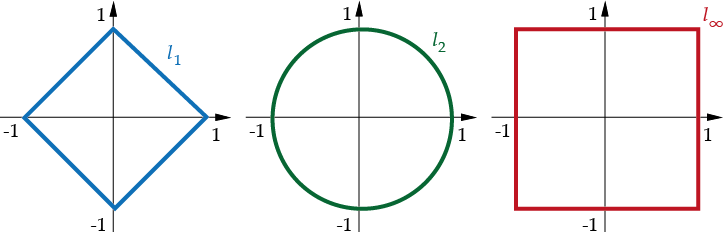
\includegraphics[width=0.7\linewidth,height=\textheight,keepaspectratio]{im/norms.png}
\end{center}

\end{fbxSimple}

\section{Matrix norms}\label{matrix-norms}

We also use norms to measure the ``size'' of matrices. Since the set
\(\mathbb{R}^{n\times n}\) of \(n\times n\) matrices with real entries
is a vector space, we could just use a vector norm on this space. But
usually we add an additional axiom.

A \textbf{matrix norm} is a real-valued function \(\|\cdot\|\) on
\(\mathbb{R}^{n\times n}\) that satisfies:

\begin{enumerate}
\def\labelenumi{\arabic{enumi}.}
\item
  \(\|A + B\| \leq \|A\| + \|B\|\) for every
  \(A,B\in\mathbb{R}^{n\times n}\).
\item
  \(\|\alpha A\| = |\alpha|\,\|A\|\) for every
  \(A\in \mathbb{R}^{n\times n}\) and every \(\alpha\in\mathbb{R}\).
\item
  \(\|A\| \geq 0\) for every \(A\in \mathbb{R}^{n\times n}\) and
  \(\|A\|=0\) implies \(A=0\).
\item
  \(\|AB\| \leq \|A\|\|B\|\) for every \(A,B\in\mathbb{R}^{n\times n}\)
  (\textbf{consistency}).
\end{enumerate}

\begin{tcolorbox}[enhanced jigsaw, bottomrule=.15mm, colbacktitle=quarto-callout-note-color!10!white, breakable, arc=.35mm, coltitle=black, colback=white, bottomtitle=1mm, opacityback=0, title=\textcolor{quarto-callout-note-color}{\faInfo}\hspace{0.5em}{Note}, titlerule=0mm, toptitle=1mm, opacitybacktitle=0.6, colframe=quarto-callout-note-color-frame, leftrule=.75mm, rightrule=.15mm, left=2mm, toprule=.15mm]

We usually want this additional axiom because matrices are more than
just vectors. Some books call this a \textbf{submultiplicative norm} and
define a ``matrix norm'' to satisfy just the first three properties,
perhaps because (4) only works for square matrices.

\end{tcolorbox}

\phantomsection\label{eg-3.10}
\begin{fbxSimple}{eg}{Example 3.10: }{Frobenius norm}
\phantomsection\label{eg-3.10}
If we treat a matrix as a big vector with \(n^2\) components, then the
\(\ell_2\)-norm is called the \textbf{Frobenius norm} of the matrix: \[
\|A\|_F = \sqrt{\sum_{i=1}^n\sum_{j=1}^n a_{ij}^2}.
\] This norm is rarely used in numerical analysis because it is not
induced by any vector norm (as we are about to define).

\end{fbxSimple}

The most important matrix norms are so-called \textbf{induced} or
\textbf{operator} norms. Remember that \(A\) is a linear map on
\(\mathbb{R}^n\), meaning that it maps every vector to another vector.
So we can measure the size of \(A\) by how much it can stretch vectors
with respect to a given vector norm. Specifically, if \(\|\cdot\|_p\) is
a vector norm, then the \textbf{induced} norm is defined as \[
\|A\|_p := \sup_{\mathbf{x}\neq \boldsymbol{0}}\frac{\|A\mathbf{x}\|_p}{\|\mathbf{x}\|_p} = \max_{\|\mathbf{x}\|_p=1}\|A\mathbf{x}\|_p.
\] To see that the two definitions here are equivalent, use the fact
that \(\|\cdot\|_p\) is a vector norm. So by property (2) we have \[
\sup_{\mathbf{x}\neq \boldsymbol{0}}\frac{\|A\mathbf{x}\|_p}{\|\mathbf{x}\|_p} = \sup_{\mathbf{x}\neq \boldsymbol{0}}\left\| A\frac{\mathbf{x}}{\|\mathbf{x}\|_p}\right\|_p = \sup_{\|\mathbf{y}\|_p=1}\|A\mathbf{y}\|_p = \max_{\|\mathbf{y}\|_p=1}\|A\mathbf{y}\|_p.
\]

\begin{tcolorbox}[enhanced jigsaw, bottomrule=.15mm, colbacktitle=quarto-callout-note-color!10!white, breakable, arc=.35mm, coltitle=black, colback=white, bottomtitle=1mm, opacityback=0, title=\textcolor{quarto-callout-note-color}{\faInfo}\hspace{0.5em}{Note}, titlerule=0mm, toptitle=1mm, opacitybacktitle=0.6, colframe=quarto-callout-note-color-frame, leftrule=.75mm, rightrule=.15mm, left=2mm, toprule=.15mm]

Usually we use the same notation for the induced matrix norm as for the
original vector norm. The meaning should be clear from the context.

\end{tcolorbox}

\phantomsection\label{eg-3.11}
\begin{fbxSimple}{eg}{Example 3.11}{}
\phantomsection\label{eg-3.11}
Let \[
A = \begin{pmatrix}
0 & 1\\
3 & 0
\end{pmatrix}.
\] In the \(\ell_2\)-norm, a unit vector in \(\mathbb{R}^2\) has the
form \(\mathbf{x}=(\cos\theta,\sin\theta)^\top\), so the image of the
unit circle is \[
A\mathbf{x} = \begin{pmatrix}
\sin\theta\\
3\cos\theta
\end{pmatrix}.
\] This is illustrated below:

\begin{center}
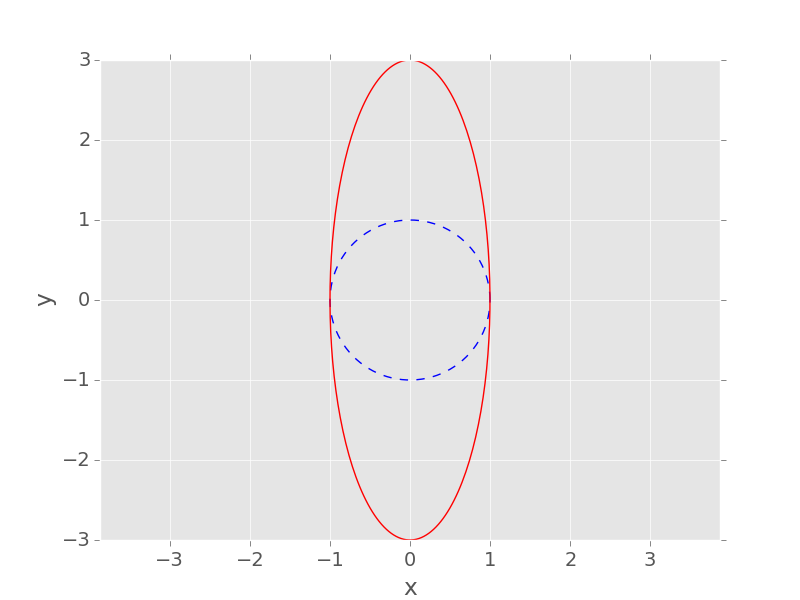
\includegraphics[width=0.6\linewidth,height=\textheight,keepaspectratio]{im/matrixnorm.png}
\end{center}

The induced matrix norm is the maximum stretching of this unit circle,
which is \[
\|A\|_2 = \max_{\|\mathbf{x}\|_2=1}\|A\mathbf{x}\|_2 = \max_\theta\big(\sin^2\theta + 9\cos^2\theta \big)^{1/2} = \max_\theta\big(1 + 8\cos^2\theta\big)^{1/2} = 3.
\]

\end{fbxSimple}

\phantomsection\label{induced-norms-are-matrix-norms}
\begin{fbxSimple}{theorem}{Theorem 3.2: }{Induced norms are matrix norms}
\phantomsection\label{induced-norms-are-matrix-norms}
The induced norm corresponding to any vector norm is a matrix norm, and
the two norms satisfy \(\|A\mathbf{x}\| \leq \|A\|\|\mathbf{x}\|\) for
any matrix \(A\in\mathbb{R}^{n\times n}\) and any vector
\(\mathbf{x}\in\mathbb{R}^n\).

\end{fbxSimple}

\textbf{Proof:}\\
Properties (1)-(3) follow from the fact that the vector norm satisfies
the corresponding properties. To show (4), note that, by the definition
above, we have for any vector \(\mathbf{y}\in\mathbb{R}^n\) that \[
\|A\| \geq \frac{\|A\mathbf{y}\|}{\|\mathbf{y}\|} \quad \implies \quad
\|A\mathbf{y}\| \leq \|A\|\|\mathbf{y}\|.
\] Taking \(\mathbf{y} = B\mathbf{x}\) for some \(\mathbf{x}\) with
\(\|\mathbf{x}\|=1\), we get \[
\|AB\mathbf{x}\|\leq\|A\|\|B\mathbf{x}\| \leq \|A\|\|B\|.
\] This holds in particular for the vector \(\mathbf{x}\) that maximises
\(\|AB\mathbf{x}\|\), so \[
\|AB\| = \max_{\|\mathbf{x}\|=1}\|AB\mathbf{x}\| \leq \|A\|\|B\|. 
\]

It is cumbersome to compute the induced norms from their definition, but
fortunately there are some very useful alternative formulae.

\phantomsection\label{matrix-norms-induced-by-ell_1-and-ell_infty}
\begin{fbxSimple}{theorem}{Theorem 3.3: }{Matrix norms induced by \(\ell_1\) and \(\ell_\infty\)}
\phantomsection\label{matrix-norms-induced-by-ell_1-and-ell_infty}
The matrix norms induced by the \(\ell_1\)-norm and \(\ell_\infty\)-norm
satisfy \[
\|A\|_1 = \max_{j=1,\ldots,n}\sum_{i=1}^n|a_{ij}|, \quad \text{(maximum column sum)}
\] \[
\|A\|_\infty = \max_{i=1,\ldots,n}\sum_{j=1}^n|a_{ij}|. \quad \text{(maximum row sum)}
\]

\end{fbxSimple}

\textbf{Proof:}\\
We will prove the result for the \(\ell_1\)-norm as an illustration of
the method: \[
\|A\mathbf{x}\|_1 = \sum_{i=1}^n\left|\sum_{j=1}^n a_{ij}x_j\right| \leq \sum_{i=1}^n\sum_{j=1}^n|a_{ij}|\,|x_j| = \sum_{j=1}^n|x_j|\sum_{i=1}^n|a_{ij}|.
\] If we let \[
c = \max_{j=1,\ldots,n}\sum_{i=1}^n|a_{ij}|,
\] then \[
\|A\mathbf{x}\|_1 \leq c\|\mathbf{x}\|_1 \quad \implies \|A\|_1 \leq c.
\] Now let \(m\) be the column where the maximum sum is attained. If we
choose \(\mathbf{y}\) to be the vector with components
\(y_k=\delta_{km}\), then we have \(\|A\mathbf{y}\|_1 = c\). Since
\(\|\mathbf{y}\|_1=1\), we must have that \[
\max_{\|\mathbf{x}\|_1=1}\|A\mathbf{x}\|_1 \geq \|A\mathbf{y}\|_1=c \quad \implies \|A\|_1 \geq c.
\] The only way to satisfy both inequalities is if \(\|A\|_1=c\).

\phantomsection\label{eg-3.12}
\begin{fbxSimple}{eg}{Example 3.12}{}
\phantomsection\label{eg-3.12}
For the matrix \[
A = \begin{pmatrix}
-7 & 3 & -1\\
2 & 4 & 5\\
-4 & 6 & 0
\end{pmatrix}
\] we have \[
\|A\|_1 = \max\{13, 13, 6\} = 13, \qquad \|A\|_\infty = \max\{11,11,10\} = 11.
\]

\end{fbxSimple}

What about the matrix norm induced by the \(\ell_2\)-norm? This turns
out to be related to the eigenvalues of \(A\). Recall that
\(\lambda\in\mathbb{C}\) is an \textbf{eigenvalue} of \(A\) with
associated \textbf{eigenvector} \(\mathbf{u}\) if \[
A\mathbf{u} = \lambda\mathbf{u}.
\] We define the \textbf{spectral radius} \(\rho(A)\) of \(A\) to be the
maximum \(|\lambda|\) over all eigenvalues \(\lambda\) of \(A\).

\phantomsection\label{spectral-norm}
\begin{fbxSimple}{theorem}{Theorem 3.4: }{Spectral norm}
\phantomsection\label{spectral-norm}
The matrix norm induced by the \(\ell_2\)-norm satisfies \[
\|A\|_2 = \sqrt{\rho(A^\top A)}.
\]

\end{fbxSimple}

As a result of the theorem above, this norm is sometimes known as the
\textbf{spectral norm}.

\phantomsection\label{eg-3.13}
\begin{fbxSimple}{eg}{Example 3.13}{}
\phantomsection\label{eg-3.13}
For our matrix \[
A = \begin{pmatrix}
0 & 1\\
3 & 0
\end{pmatrix},
\] we have \[
A^\top A = \begin{pmatrix}
0 & 3\\
1 & 0
\end{pmatrix}
\begin{pmatrix}
0 & 1\\
3 & 0
\end{pmatrix}
=\begin{pmatrix}
9 & 0\\
0 & 1
\end{pmatrix}.
\] We see that the eigenvalues of \(A^\top A\) are \(\lambda=1,9\), so
\(\|A\|_2=\sqrt{9}=3\) (as we calculated earlier).

\end{fbxSimple}

\textbf{Proof:}\\
We want to show that \[
\max_{\|\mathbf{x}\|_2 = 1}\|A\mathbf{x}\|_2  = \max\{\sqrt{|\lambda|} \,: \,\textrm{$\lambda$ eigenvalue of $A^\top A$} \}.
\] For \(A\) real, \(A^\top A\) is symmetric, so has real eigenvalues
\(\lambda_1 \leq\lambda_2 \leq \ldots \leq \lambda_n\) with
corresponding orthonormal eigenvectors
\(\mathbf{u}_1, \ldots,\mathbf{u}_n\) in \(\mathbb{R}^n\). (Orthonormal
means that \(\mathbf{u}_j^\top \mathbf{u}_k = \delta_{jk}\).) Note also
that all of the eigenvalues are non-negative, since \[
A^\top A\mathbf{u}_1 = \lambda_1\mathbf{u}_1 \quad \implies \lambda_1 = \frac{\mathbf{u}_1^\top A^\top A\mathbf{u}_1}{\mathbf{u}_1^\top\mathbf{u}_1} = \frac{\|A\mathbf{u}_1\|_2^2}{\|\mathbf{u}_1\|_2^2} \geq 0.
\] So we want to show that \(\|A\|_2=\sqrt{\lambda_n}\). The
eigenvectors form a basis, so every vector \(\mathbf{x}\in\mathbb{R}^n\)
can be expressed as a linear combination
\(\mathbf{x} = \sum_{k=1}^n\alpha_k\mathbf{u}_k\). Therefore \[
\|A\mathbf{x}\|_2^2 = \mathbf{x}^\top A^\top A\mathbf{x} = \mathbf{x}^\top\sum_{k=1}^n\alpha_k\lambda_k\mathbf{u}_k = \sum_{j=1}^n\alpha_j\mathbf{u}_j^\top\sum_{k=1}^n\alpha_k\lambda_k\mathbf{u}_k = \sum_{k=1}^n\alpha_k^2\lambda_k,
\] where the last step uses orthonormality of the \(\mathbf{u}_k\). It
follows that \[
\|A\mathbf{x}\|_2^2 \leq \lambda_n\sum_{k=1}^n\alpha_k^2.
\] But if \(\|\mathbf{x}\|_2=1\), then
\(\|\mathbf{x}\|_2^2=\sum_{k=1}^n\alpha_k^2 = 1\), so
\(\|A\mathbf{x}\|_2^2 \leq \lambda_n\). To show that the maximum of
\(\|A\mathbf{x}\|_2^2\) is equal to \(\lambda_n\), we can choose
\(\mathbf{x}\) to be the corresponding eigenvector
\(\mathbf{x}=\mathbf{u}_n\). In that case,
\(\alpha_1=\ldots=\alpha_{n-1}=0\) and \(\alpha_n=1\), so
\(\|A\mathbf{x}\|_2^2 =\lambda_n\).

\section{Conditioning}\label{conditioning}

Some linear systems are inherently more difficult to solve than others,
because the solution is sensitive to small perturbations in the input.
We will examine how to quantify this sensitivity and how to adjust our
methods to control for it.

\phantomsection\label{eg-3.14}
\begin{fbxSimple}{eg}{Example 3.14}{}
\phantomsection\label{eg-3.14}
Consider the linear system \[
\begin{pmatrix}
1 & 1\\
0 & 1
\end{pmatrix}
\begin{pmatrix}
x_1\\ x_2
\end{pmatrix}
= \begin{pmatrix}
1\\ 1
\end{pmatrix}
\implies
\begin{pmatrix}
x_1\\ x_2
\end{pmatrix}= 
\begin{pmatrix}
0\\ 1
\end{pmatrix}.
\] If we add a small rounding error \(0<\delta \ll 1\) to the data
\(b_1\) then \[
\begin{pmatrix}
1 & 1\\
0 & 1
\end{pmatrix}
\begin{pmatrix}
x_1\\ x_2
\end{pmatrix}
= \begin{pmatrix}
1 + \delta\\ 1
\end{pmatrix}
\implies
\begin{pmatrix}
x_1\\ x_2
\end{pmatrix}= 
\begin{pmatrix}
\delta\\ 1
\end{pmatrix}.
\] The solution is within rounding error of the true solution, so the
system is called \textbf{well conditioned}.

\end{fbxSimple}

\phantomsection\label{eg-3.15}
\begin{fbxSimple}{eg}{Example 3.15}{}
\phantomsection\label{eg-3.15}
Now let \(\epsilon \ll 1\) be a fixed positive number, and consider the
linear system \[
\begin{pmatrix}
\epsilon & 1\\
0 & 1
\end{pmatrix}
\begin{pmatrix}
x_1\\ x_2
\end{pmatrix}
= \begin{pmatrix}
1 + \delta\\ 1
\end{pmatrix}
\implies
\begin{pmatrix}
x_1\\ x_2
\end{pmatrix}= 
\begin{pmatrix}
\delta/\epsilon\\ 1
\end{pmatrix}.
\] The true solution is still \((0,1)^\top\), but if the error
\(\delta\) is as big as the matrix entry \(\epsilon\), then the solution
for \(x_1\) will be completely wrong. This system is much more sensitive
to errors in \(\mathbf{b}\), so is called \textbf{ill-conditioned}.

Graphically, this system (right) is more sensitive to \(\delta\) than
the first system (left) because the two lines are closer to parallel:

\begin{center}
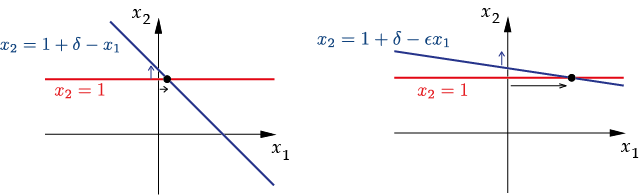
\includegraphics[width=0.8\linewidth,height=\textheight,keepaspectratio]{im/conditioning.png}
\end{center}

\end{fbxSimple}

To measure the \textbf{conditioning} of a linear system, consider the
following estimate of the ratio of the relative errors in the output
(\(x\)) versus the input (\(b\)): \[
\begin{aligned}
\frac{|\textrm{relative error in }\mathbf{x}|}{|\textrm{relative error in }\mathbf{b}|}
&= \frac{\|\delta\mathbf{x}\|/\|\mathbf{x}\|}{\|\delta\mathbf{b}\|/\|\mathbf{b}\|}
= \left(\frac{\|\delta\mathbf{x}\|}{\|\mathbf{x}\|}\right)\left(\frac{\|\mathbf{b}\|}{\|\delta\mathbf{b}\|} \right) \\
&= \left(\frac{\|A^{-1}\delta\mathbf{b}\|}{\|\mathbf{x}\|}\right)\left(\frac{\|\mathbf{b}\|}{\|\delta\mathbf{b}\|} \right) \\
&\leq \frac{\|A^{-1}\|\|\delta\mathbf{b}\|}{\|\mathbf{x}\|}\left(\frac{\|\mathbf{b}\|}{\|\delta\mathbf{b}\|} \right) \\
&= \frac{\|A^{-1}\|\|\mathbf{b}\|}{\|\mathbf{x}\|} = \frac{\|A^{-1}\|\|A\mathbf{x}\|}{\|\mathbf{x}\|}\\
&\leq \|A^{-1}\|\|A\|.
\end{aligned}
\]

We define the \textbf{condition number} of a matrix \(A\) in some
induced norm \(\|\cdot\|_*\) to be \[
\kappa_*(A) = \|A^{-1}\|_*\|A\|_*.
\] If \(\kappa_*(A)\) is large, then the solution will be sensitive to
errors in \(\mathbf{b}\), at least for some \(\mathbf{b}\). A large
condition number means that the matrix is close to being non-invertible
(i.e.~two rows are close to being linearly dependent).

\begin{tcolorbox}[enhanced jigsaw, bottomrule=.15mm, colbacktitle=quarto-callout-note-color!10!white, breakable, arc=.35mm, coltitle=black, colback=white, bottomtitle=1mm, opacityback=0, title=\textcolor{quarto-callout-note-color}{\faInfo}\hspace{0.5em}{Note}, titlerule=0mm, toptitle=1mm, opacitybacktitle=0.6, colframe=quarto-callout-note-color-frame, leftrule=.75mm, rightrule=.15mm, left=2mm, toprule=.15mm]

This is a ``worst case'' amplification of the error by a given matrix.
The actual result will depend on \(\delta\mathbf{b}\) (which we usually
don't know if it arises from previous rounding error).

\end{tcolorbox}

Note that \(\det(A)\) will tell you whether a matrix is singular or not,
but not whether it is ill-conditioned. Since
\(\det(\alpha A) = \alpha^n\det(A)\), the determinant can be made
arbitrarily large or small by scaling (which does not change the
condition number). For instance, the matrix \[
\begin{pmatrix}
10^{-50} & 0\\
0 & 10^{-50}
\end{pmatrix}
\] has tiny determinant but is well-conditioned.

\phantomsection\label{eg-3.16}
\begin{fbxSimple}{eg}{Example 3.16}{}
\phantomsection\label{eg-3.16}
Return to our earlier examples and consider the condition numbers in the
1-norm.

We have (assuming \(0< \epsilon \ll 1\)) that \[
A = \begin{pmatrix}
1 & 1\\
0 & 1
\end{pmatrix} \implies
A^{-1} = \begin{pmatrix}
1 & -1\\
0 & 1
\end{pmatrix} \implies
\|A\|_1 = \|A^{-1}\|_1 = 2 \implies \kappa_1(A) = 4,
\] \[
B = \begin{pmatrix}
\epsilon & 1\\
0 & 1
\end{pmatrix} \implies
B^{-1} = \frac{1}{\epsilon}\begin{pmatrix}
1 & -1\\
0 & \epsilon
\end{pmatrix} 
\] \[
\implies
\|B\|_1 = 2, \,\, \|B^{-1}\|_1 = \frac{1 + \epsilon}{\epsilon} \implies \kappa_1(B) = \frac{2(1+\epsilon)}{\epsilon}.
\] For matrix \(B\), \(\kappa_1(B)\to\infty\) as \(\epsilon\to 0\),
showing that the matrix \(B\) is ill-conditioned.

\end{fbxSimple}

\phantomsection\label{eg-3.17}
\begin{fbxSimple}{eg}{Example 3.17}{}
\phantomsection\label{eg-3.17}
The \textbf{Hilbert matrix} \(H_n\) is the \(n\times n\) symmetric
matrix with entries \[
(h_n)_{ij} = \frac{1}{i+j-1}.
\] These matrices are notoriously ill-conditioned. For example,
\(\kappa_2(H_5) \approx 4.8\times 10^5\), and
\(\kappa_2(H_{20})\approx 2.5\times 10^{28}\). Solving an associated
linear system in floating-point arithmetic would be hopeless.

\end{fbxSimple}

A practical limitation of the condition number is that you have to know
\(A^{-1}\) before you can calculate it. We can always estimate
\(\|A^{-1}\|\) by taking some arbitrary vectors \(\mathbf{x}\) and using
\[
\|A^{-1}\| \geq \frac{\|\mathbf{x}\|}{\|\mathbf{b}\|}.
\]

\section{Iterative methods}\label{iterative-methods}

For large systems, the \({\cal O}(n^3)\) cost of Gaussian elimination is
prohibitive. Fortunately, many such systems that arise in practice are
\textbf{sparse}, meaning that most of the entries of the matrix \(A\)
are zero. In this case, we can often use iterative algorithms to do
better than \({\cal O}(n^3)\).

In this course, we will only study algorithms for symmetric positive
definite matrices. A matrix \(A\) is called \textbf{symmetric positive
definite} (or \textbf{SPD}) if \(\mathbf{x}^\top A\mathbf{x}>0\) for
every vector \(\mathbf{x}\neq 0\).

\begin{tcolorbox}[enhanced jigsaw, bottomrule=.15mm, colbacktitle=quarto-callout-note-color!10!white, breakable, arc=.35mm, coltitle=black, colback=white, bottomtitle=1mm, opacityback=0, title=\textcolor{quarto-callout-note-color}{\faInfo}\hspace{0.5em}{Note}, titlerule=0mm, toptitle=1mm, opacitybacktitle=0.6, colframe=quarto-callout-note-color-frame, leftrule=.75mm, rightrule=.15mm, left=2mm, toprule=.15mm]

Recall that a symmetric matrix has real eigenvalues. It is positive
definite iff all of its eigenvalues are positive.

\end{tcolorbox}

\phantomsection\label{eg-3.18}
\begin{fbxSimple}{eg}{Example 3.18}{}
\phantomsection\label{eg-3.18}
Show that the following matrix is SPD: \[
A = \begin{pmatrix}
3 & 1 & -1\\
1 & 4 & 2\\
-1 & 2 & 5
\end{pmatrix}.
\] With \(\mathbf{x} = (x_1,x_2,x_3)^\top\), we have \[
\begin{aligned}
\mathbf{x}^\top A\mathbf{x} &= 3x_1^2 + 4x_2^2 + 5x_3^2 + 2x_1x_2 + 4x_2x_3 - 2x_1x_3\\
&= x_1^2 + x_2^2 + 2x_3^2 + (x_1+x_2)^2 + (x_1-x_3)^2 + 2(x_2+x_3)^2.
\end{aligned}
\] This is positive for any non-zero vector
\(\mathbf{x}\in\mathbb{R}^3\), so \(A\) is SPD (eigenvalues \(1.29\),
\(4.14\) and \(6.57\)).

\end{fbxSimple}

If \(A\) is SPD, then solving \(A\mathbf{x} = \mathbf{b}\) is equivalent
to minimizing the quadratic functional \[
f:\mathbb{R}^n \to \mathbb{R}, \qquad f(\mathbf{x}) = \tfrac12\mathbf{x}^\top A\mathbf{x} -\mathbf{b}^\top\mathbf{x}.
\] When \(A\) is SPD, this functional behaves like a U-shaped parabola,
and has a unique finite global minimizer \(\mathbf{x}_*\) such that
\(f(\mathbf{x}_*)< f(\mathbf{x})\) for all
\(\mathbf{x}\in\mathbb{R}^n\), \(\mathbf{x}\neq\mathbf{x}_*\).

To find \(\mathbf{x}_*\), we need to set \(\nabla f = \boldsymbol{0}\).
We have \[
f(\mathbf{x}) = \tfrac12\sum_{i=1}^n x_i\left(\sum_{j=1}^n a_{ij}x_j\right) - \sum_{j=1}^nb_jx_j
\] so \[
\begin{aligned}
\frac{\partial f}{\partial x_k} &= \tfrac12\left(\sum_{i=1}^n x_ia_{ik} + \sum_{j=1}^na_{kj}x_j \right) - b_k \\ &= \tfrac12\left(\sum_{i=1}^n a_{ki}x_i + \sum_{j=1}^na_{kj}x_j \right) - b_k = \sum_{j=1}^na_{kj}x_j - b_k.
\end{aligned}
\] In the penultimate step we used the symmetry of \(A\) to write
\(a_{ik}=a_{ki}\). It follows that \[
\nabla f = A\mathbf{x} - \mathbf{b},
\] so locating the minimum of \(f(\mathbf{x})\) is indeed equivalent to
solving \(A\mathbf{x}=\mathbf{b}\).

\begin{tcolorbox}[enhanced jigsaw, bottomrule=.15mm, colbacktitle=quarto-callout-note-color!10!white, breakable, arc=.35mm, coltitle=black, colback=white, bottomtitle=1mm, opacityback=0, title=\textcolor{quarto-callout-note-color}{\faInfo}\hspace{0.5em}{Note}, titlerule=0mm, toptitle=1mm, opacitybacktitle=0.6, colframe=quarto-callout-note-color-frame, leftrule=.75mm, rightrule=.15mm, left=2mm, toprule=.15mm]

Minimizing functions is a vast sub-field of numerical analysis known as
\textbf{optimization}. We will only cover this specific case.

\end{tcolorbox}

A popular class of methods for optimization are \textbf{line search}
methods, where at each iteration the search is restricted to a single
\textbf{search direction} \(\mathbf{d}_k\). The iteration takes the form
\[
\mathbf{x}_{k+1} = \mathbf{x}_k + \alpha_k\mathbf{d}_k.
\] The \textbf{step size} \(\alpha_k\) is chosen by minimizing
\(f(\mathbf{x})\) along the line
\(\mathbf{x} = \mathbf{x}_k + \alpha\mathbf{d}_k\). For our functional
above, we have \[
\begin{aligned}
f(\mathbf{x}_{k} + \alpha\mathbf{d}_{k}) &= \big(\tfrac12\mathbf{d}_{k}^\top A\mathbf{d}_{k}\big)\alpha^2 + \mathbf{d}_{k}^\top\big(  A\mathbf{x}_k - \mathbf{b} \big)\alpha + \tfrac12\mathbf{x}_k^\top A\mathbf{x}_k - \mathbf{b}^\top\mathbf{x}_k.
\end{aligned}
\] This is a quadratic in \(\alpha\), and the coefficient of
\(\alpha^2\) is positive because \(A\) is positive definite. It is
therefore a U-shaped parabola and achieves its minimum when \[
\frac{\partial f}{\partial\alpha} = \mathbf{d}_k^\top A\mathbf{d}_k \alpha + \mathbf{d}_k^\top\big(A\mathbf{x}_k - \mathbf{b}\big) = 0.
\] Defining the \textbf{residual}
\(\mathbf{r}_k := A\mathbf{x}_k - \mathbf{b}\), we see that the desired
choice of step size is \[
\alpha_k = - \frac{\mathbf{d}_k^\top\mathbf{r}_k}{\mathbf{d}_k^\top A\mathbf{d}_k}.
\]

Different line search methods differ in how the search direction
\(\mathbf{d}_k\) is chosen at each iteration. For example, the
\textbf{method of steepest descent} sets \[
\mathbf{d}_k = - \nabla f (\mathbf{x}_k) = -\mathbf{r}_k,
\] where we have remembered the gradient formula above.

\phantomsection\label{eg-3.19}
\begin{fbxSimple}{eg}{Example 3.19}{}
\phantomsection\label{eg-3.19}
Use the method of steepest descent to solve the system \[
\begin{pmatrix}
3 & 2\\ 2 & 6
\end{pmatrix}\begin{pmatrix}
x_1\\ x_2
\end{pmatrix}=\begin{pmatrix}
2\\ -8
\end{pmatrix}.
\] Starting from \(\mathbf{x}_0=(-2,-2)^\top\), we get \[
\begin{aligned}
\mathbf{d}_0 = \mathbf{b} - A\mathbf{x}_0 = \begin{pmatrix}
12\\ 8
\end{pmatrix} &\implies \alpha_0 = \frac{\mathbf{d}_0^\top\mathbf{d}_0}{\mathbf{d}_0^\top A\mathbf{d}_0} = \frac{208}{1200} \\ &\implies \mathbf{x}_1 = \mathbf{x}_0 + \alpha_0\mathbf{d}_0 \approx \begin{pmatrix}
0.08\\ -0.613
\end{pmatrix}.
\end{aligned}
\] Continuing the iteration, \(\mathbf{x}_k\) proceeds towards the
solution \((2,-2)^\top\) as illustrated below. The coloured contours
show the value of \(f(x_1,x_2)\).

\begin{center}
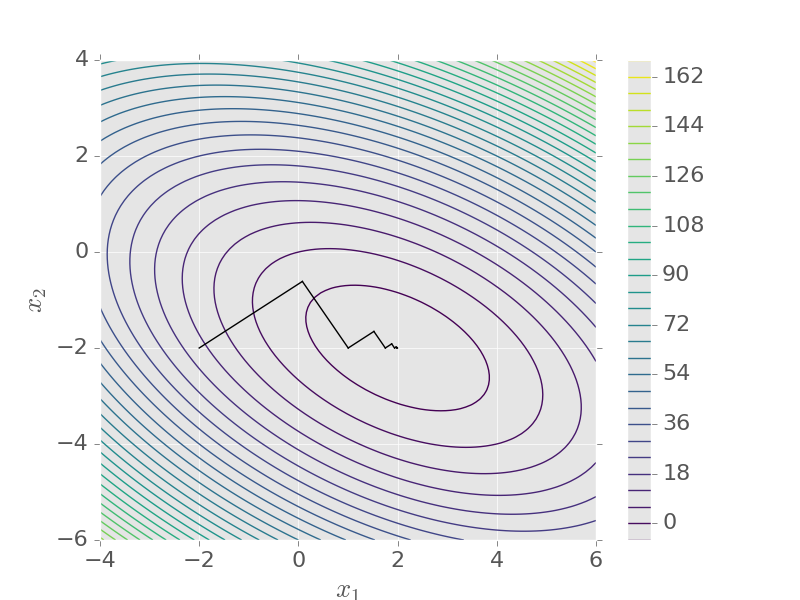
\includegraphics[width=0.7\linewidth,height=\textheight,keepaspectratio]{im/linear_steepest.png}
\end{center}

\end{fbxSimple}

Unfortunately, the method of steepest descent can be slow to converge.
In the \textbf{conjugate gradient method}, we still take
\(\mathbf{d}_0=-\mathbf{r}_0\), but subsequent search directions
\(\mathbf{d}_k\) are chosen to be \textbf{\(A\)-conjugate}, meaning that
\[
\mathbf{d}_{k+1}^\top A \mathbf{d}_k = 0.
\] This means that minimization in one direction does not undo the
previous minimizations.

In particular, we construct \(\mathbf{d}_{k+1}\) by writing \[
\mathbf{d}_{k+1} = -\mathbf{r}_{k+1} + \beta_k\mathbf{d}_k,
\] then choosing the scalar \(\beta_k\) such that
\(\mathbf{d}_{k+1}^\top A\mathbf{d}_k = 0\). This gives \[
0 = \big(-\mathbf{r}_{k+1} + \beta_k\mathbf{d}_k\big)^\top A \mathbf{d}_{k} = -\mathbf{r}_{k+1}^\top A \mathbf{d}_k + \beta_k\mathbf{d}_k^\top A \mathbf{d}_k
\] and hence \[
\beta_k = \frac{\mathbf{r}_{k+1}^\top A\mathbf{d}_k}{\mathbf{d}_k^\top A \mathbf{d}_k}.
\]

Thus we get the basic conjugate gradient algorithm.

\phantomsection\label{algorithm-3.2}
\begin{fbxSimple}{algorithm}{Algorithm 3.2: }{Conjugate gradient method}
\phantomsection\label{algorithm-3.2}

Start with an initial guess \(\mathbf{x}_0\) and initial search
direction \(\mathbf{d}_0 = -\mathbf{r}_0 = \mathbf{b} - A\mathbf{x}_0\).
For each \(k=0,1,\ldots\), do the following:

\begin{enumerate}
\def\labelenumi{\arabic{enumi}.}
\item
  Compute step size \[
  \alpha_k = -\frac{\mathbf{d}_k^\top\mathbf{r}_k}{\mathbf{d}_k^\top A \mathbf{d}_k}.
  \]
\item
  Compute \(\mathbf{x}_{k+1} = \mathbf{x}_k + \alpha_k\mathbf{d}_k\).
\item
  Compute residual
  \(\mathbf{r}_{k+1} = A\mathbf{x}_{k+1} - \mathbf{b}\).
\item
  If \(\|\mathbf{r}_{k+1}\| <\) tolerance, output \(\mathbf{x}_{k+1}\)
  and stop.
\item
  Determine new search direction \[
  \mathbf{d}_{k+1} = -\mathbf{r}_{k+1} + \beta_k\mathbf{d}_k \quad \textrm{where} \quad\beta_k = \frac{\mathbf{r}_{k+1}^\top A \mathbf{d}_k}{\mathbf{d}_k^\top A \mathbf{d}_k}.
  \]
\end{enumerate}

\end{fbxSimple}

\phantomsection\label{eg-3.20}
\begin{fbxSimple}{eg}{Example 3.20}{}
\phantomsection\label{eg-3.20}
Solve our previous example with the conjugate gradient method.

Starting with \(\mathbf{x}_0=(-2,-2)^\top\), the first step is the same
as in steepest descent, giving \(\mathbf{x}_1 = (0.08, -0.613)^\top\).
But then we take \[
\mathbf{r}_1 = A\mathbf{x}_1 -\mathbf{b} = \begin{pmatrix}
-2.99\\ 4.48
\end{pmatrix}, \quad \beta_0 = \frac{\mathbf{r}_1^\top A\mathbf{d}_0}{\mathbf{d}_0^\top A\mathbf{d}_0} = 0.139, \quad \mathbf{d}_1 = -\mathbf{r}_1 + \beta_0\mathbf{d}_0 = \begin{pmatrix}
4.66\\-3.36
\end{pmatrix}.
\] The second iteration then gives \[
\alpha_1 = -\frac{\mathbf{d}_1^\top\mathbf{r}_1}{\mathbf{d}_1^\top A\mathbf{d}_1} = 0.412 \implies \mathbf{x}_2 = \mathbf{x}_1 + \alpha_1\mathbf{d}_1 = \begin{pmatrix}
2\\-2
\end{pmatrix}.
\] This time there is no zig-zagging and the solution is reached in just
two iterations:

\begin{center}
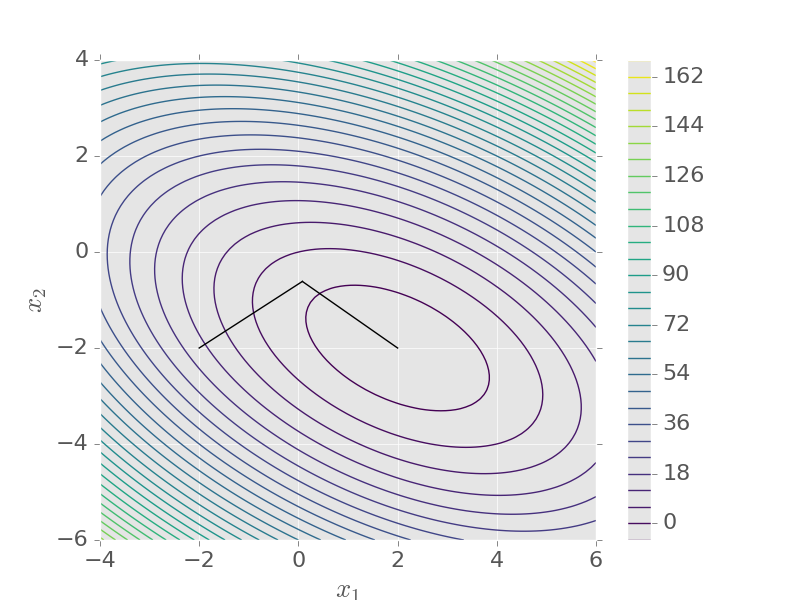
\includegraphics[width=0.7\linewidth,height=\textheight,keepaspectratio]{im/linear_cg.png}
\end{center}

\end{fbxSimple}

In exact arithmetic, the conjugate gradient method will always give the
exact answer in \(n\) iterations -- one way to see this is to use the
following.

\phantomsection\label{theorem-3.5}
\begin{fbxSimple}{theorem}{Theorem 3.5}{}
\phantomsection\label{theorem-3.5}
The residuals \(\mathbf{r}_k:=A\mathbf{x}_k - \mathbf{b}\) at each stage
of the conjugate gradient method are mutually orthogonal, meaning
\(\mathbf{r}_j^\top \mathbf{r}_k = 0\) for \(j=0,\ldots,k-1\).

\end{fbxSimple}

After \(n\) iterations, the only residual vector that can be orthogonal
to all of the previous ones is \(\mathbf{r}_n=\boldsymbol{0}\), so
\(\mathbf{x}_n\) must be the exact solution.

In practice, conjugate gradients is not competitive as a direct method.
It is computationally intensive, and rounding errors can destroy the
orthogonality, meaning that more than \(n\) iterations may be required.
Instead, its main use is for large sparse systems. For suitable matrices
(perhaps after \textbf{preconditioning}), it can converge very rapidly.

We can save computation by using the alternative formulae \[
\mathbf{r}_{k+1} = \mathbf{r}_k + \alpha_k A\mathbf{d}_k, \quad
\alpha_k = \frac{\mathbf{r}_k^\top \mathbf{r}_k}{\mathbf{d}_k^\top A \mathbf{d}_k}, \quad
\beta_k = \frac{\mathbf{r}_{k+1}^\top\mathbf{r}_{k+1}}{\mathbf{r}_k^\top\mathbf{r}_k}.
\] With these formulae, each iteration requires only one matrix-vector
product, two vector-vector products, and three vector additions. Compare
this to the basic algorithm above which requires two matrix-vector
products, four vector-vector products and three vector additions.

\section*{Knowledge checklist}\label{knowledge-checklist-2}
\addcontentsline{toc}{section}{Knowledge checklist}

\markright{Knowledge checklist}

\textbf{Key topics:}

\begin{enumerate}
\def\labelenumi{\arabic{enumi}.}
\item
  Direct and iterative methods for solving linear systems: triangular
  systems, Gaussian elimination, LU decomposition, and iterative
  algorithms.
\item
  Vector and matrix norms, including induced matrix norms and their role
  in error analysis.
\item
  Conditioning and the condition number: sensitivity of solutions to
  input errors and implications for numeric stability.
\end{enumerate}

\textbf{Key skills:}

\begin{itemize}
\item
  Formulate and solve linear systems using direct and iterative methods
  (e.g., Gaussian elimination, LU decomposition).
\item
  Apply norms to measure errors and conditioning, and calculate
  condition numbers.
\item
  Analyze computational complexity and efficiency of matrix algorithms.
\end{itemize}

\bookmarksetup{startatroot}

\chapter{Calculus}\label{calculus}

\section{Differentiation}\label{s-diff}

\begin{quote}
\emph{How do we differentiate functions numerically?}
\end{quote}

\subsection{Basics}\label{basics}

The definition of the derivative as \[
f'(x_0) = \lim_{h\to 0}\frac{f(x_0+h) - f(x_0)}{h},
\] suggests an obvious approximation: just pick some small finite \(h\)
to give the estimate \[
f'(x_0) \approx \frac{f(x_0 + h) - f(x_0)}{h}.
\] For \(h>0\) this is called a \textbf{forward difference} (and, for
\(h<0\), a \textbf{backward difference}). It is an example of a
\textbf{finite-difference formula}.

\begin{center}
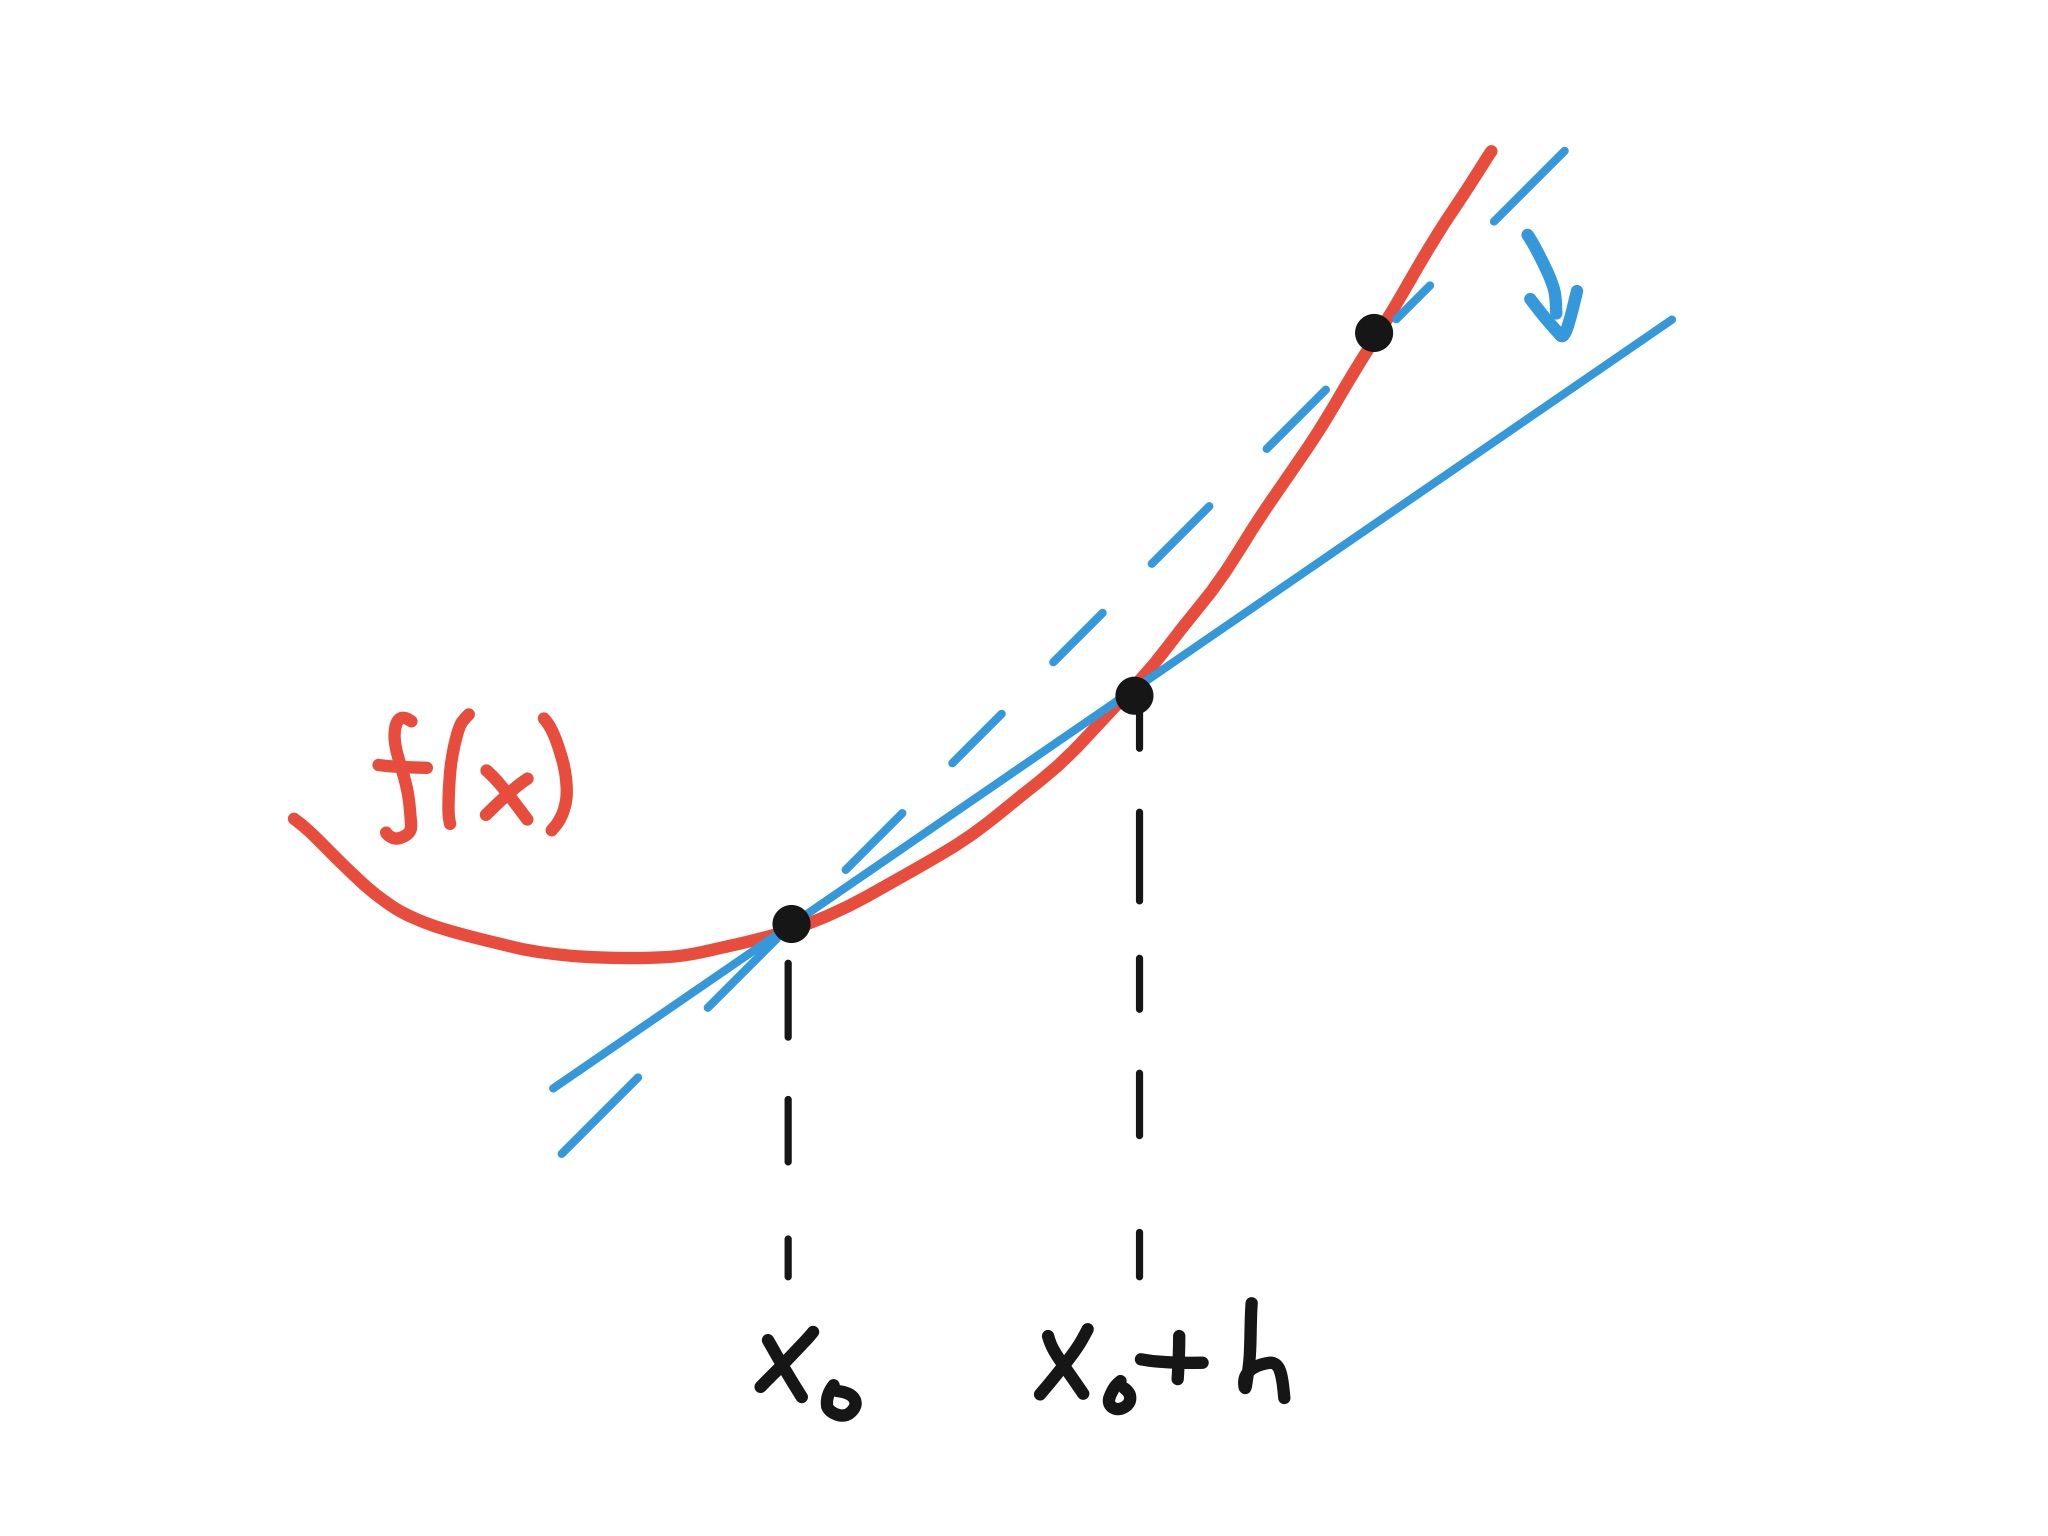
\includegraphics[width=0.6\linewidth,height=\textheight,keepaspectratio]{im/diff.jpg}
\end{center}

Of course, what we are doing with the forward difference is
approximating \(f'(x_0)\) by the slope of the linear interpolant for
\(f\) at the nodes \(x_0\) and \(x_1=x_0 + h\). So we could also have
derived the forward difference formula by starting with the Lagrange
form of the interpolating polynomial, \[
f(x) = \frac{x-x_1}{x_0-x_1}f(x_0) + \frac{x-x_0}{x_1-x_0}f(x_1) + \frac{f''(\xi)}{2}(x-x_0)(x-x_1)
\] for some \(\xi\in[x_0,x_1]\). Differentiating -- and remembering that
\(\xi\) depends on \(x\), so that we need to use the chain rule -- we
get \[
\begin{aligned}
f'(x) &= \frac{1}{x_0-x_1}f(x_0) + \frac{1}{x_1-x_0}f(x_1) + \frac{f''(\xi)}{2}(2x - x_0 - x_1) \\
&\quad + \frac{f'''(\xi)}{2}\left(\frac{\mathrm{d}\xi}{\mathrm{d}x}\right)(x-x_0)(x-x_1),\\
&\implies f'(x_0) = \frac{f(x_1) - f(x_0)}{x_1-x_0} + f''(\xi)\frac{x_0-x_1}{2}.
\end{aligned}
\] Equivalently, \[
f'(x_0) = \frac{f(x_0+h)-f(x_0)}{h} - f''(\xi)\frac{h}{2}.
\] This shows that the \textbf{truncation error} for our forward
difference approximation is \(-f''(\xi)h/2\), for some
\(\xi\in[x_0,x_0+h]\). In other words, a smaller interval or a less
``wiggly'' function will lead to a better estimate, as you would expect.

Another way to estimate the truncation error is to use Taylor's theorem,
which tells us that \[
f(x_0+h) = f(x_0) + h f'(x_0) + h^2\frac{f''(\xi)}{2},
\] for some \(\xi\) between \(x_0\) and \(x_0+h\). Rearranging this will
give back the forward difference error formula.

\phantomsection\label{derivative-of-fxlogx-at-x_02.}
\begin{fbxSimple}{eg}{Example 4.1: }{Derivative of \(f(x)=\log(x)\) at \(x_0=2\).}
\phantomsection\label{derivative-of-fxlogx-at-x_02.}
Using a forward-difference, we get the following sequence of
approximations:

\begin{longtable}[]{@{}lll@{}}
\toprule\noalign{}
\(h\) & Forward difference & Truncation error \\
\midrule\noalign{}
\endhead
\bottomrule\noalign{}
\endlastfoot
1 & 0.405465 & 0.0945349 \\
0.1 & 0.487902 & 0.0120984 \\
0.01 & 0.498754 & 0.00124585 \\
0.001 & 0.499875 & 0.000124958 \\
\end{longtable}

Indeed the error is linear in \(h\), and we estimate that it is
approximately \(0.125 h\) when \(h\) is small. This agrees with the
error formula above, since \(f''(x) = -x^{-2}\), so we expect
\(-f''(\xi)/2\approx \tfrac18\).

\end{fbxSimple}

Since the error is linearly proportional to \(h\), the approximation is
called \textbf{linear}, or \textbf{first order}.

\subsection{Higher-order finite
differences}\label{higher-order-finite-differences}

To get a higher-order approximation, we can differentiate a higher
degree interpolating polynomial. This means that we need more nodes.

\phantomsection\label{central-difference}
\begin{fbxSimple}{eg}{Example 4.2: }{Central difference}
\phantomsection\label{central-difference}
Take three nodes \(x_0\), \(x_1=x_0+h\), and \(x_2=x_0+2h\). Then the
Lagrange form of the interpolating polynomial is \[
\begin{aligned}
f(x) &= \frac{(x-x_1)(x-x_2)}{(x_0-x_1)(x_0-x_2)}f(x_0) + \frac{(x-x_0)(x-x_2)}{(x_1-x_0)(x_1-x_2)}f(x_1)\\ &+ \frac{(x-x_0)(x-x_1)}{(x_2-x_0)(x_2-x_1)}f(x_2) \\
&+ \frac{f'''(\xi)}{3!}(x-x_0)(x-x_1)(x-x_2).
\end{aligned}
\] Differentiating, we get \[
\begin{aligned}
f'(x) &= \frac{2x - x_1 - x_2}{(x_0-x_1)(x_0-x_2)}f(x_0)\\ &+ \frac{2x - x_0 - x_2}{(x_1-x_0)(x_1-x_2)}f(x_1)\\ &+ \frac{2x-x_0-x_1}{(x_2-x_0)(x_2-x_1)}f(x_2)\\
&+ \frac{f'''(\xi)}{6}\Big((x-x_1)(x-x_2) + (x-x_0)(x-x_2) + (x-x_0)(x-x_1) \Big) \\
&+ \frac{f^{(4)}(\xi)}{6}\left(\frac{\mathrm{d}\xi}{\mathrm{d}x}\right)(x-x_0)(x-x_1)(x-x_2).
\end{aligned}
\] Now substitute in \(x=x_1\) to evaluate this at the central point: \[
\begin{aligned}
f'(x_1) &= \frac{x_1 - x_2}{(x_0-x_1)(x_0-x_2)}f(x_0)\\ &+ \frac{2x_1 - x_0 - x_2}{(x_1-x_0)(x_1-x_2)}f(x_1) + \frac{x_1-x_0}{(x_2-x_0)(x_2-x_1)}f(x_2)\\
&+ \frac{f'''(\xi)}{6}(x_1-x_0)(x_1-x_2),\\
&= \frac{-h}{2h^2}f(x_0) + 0 + \frac{h}{2h^2}f(x_2) - \frac{f'''(\xi)}{6}h^2\\
&= \frac{f(x_1+h) - f(x_1-h)}{2h} - \frac{f'''(\xi)}{6}h^2.
\end{aligned}
\] This is called a \textbf{central difference} approximation for
\(f'(x_1)\), and is frequently used in practice.

\end{fbxSimple}

To see the quadratic behaviour of the truncation error, go back to our
earlier example.

\phantomsection\label{derivative-of-fxlogx-at-x2}
\begin{fbxSimple}{eg}{Example 4.3: }{Derivative of \(f(x)=\log(x)\) at \(x=2\)}
\phantomsection\label{derivative-of-fxlogx-at-x2}

\begin{longtable}[]{@{}
  >{\raggedright\arraybackslash}p{(\linewidth - 8\tabcolsep) * \real{0.0864}}
  >{\raggedright\arraybackslash}p{(\linewidth - 8\tabcolsep) * \real{0.2346}}
  >{\raggedright\arraybackslash}p{(\linewidth - 8\tabcolsep) * \real{0.2222}}
  >{\raggedright\arraybackslash}p{(\linewidth - 8\tabcolsep) * \real{0.2346}}
  >{\raggedright\arraybackslash}p{(\linewidth - 8\tabcolsep) * \real{0.2222}}@{}}
\toprule\noalign{}
\begin{minipage}[b]{\linewidth}\raggedright
\(h\)
\end{minipage} & \begin{minipage}[b]{\linewidth}\raggedright
Forward difference
\end{minipage} & \begin{minipage}[b]{\linewidth}\raggedright
Truncation error
\end{minipage} & \begin{minipage}[b]{\linewidth}\raggedright
Central difference
\end{minipage} & \begin{minipage}[b]{\linewidth}\raggedright
Truncation error
\end{minipage} \\
\midrule\noalign{}
\endhead
\bottomrule\noalign{}
\endlastfoot
1 & 0.405465 & 0.0945349 & 0.549306 & -0.0493061 \\
0.1 & 0.487902 & 0.0120984 & 0.500417 & -0.000417293 \\
0.01 & 0.498754 & 0.00124585 & 0.500004 & -4.16673e-06 \\
0.001 & 0.499875 & 0.000124958 & 0.500000 & -4.16666e-08 \\
\end{longtable}

The truncation error for the central difference is about \(0.04h^2\),
which agrees with the formula since
\(f'''(\xi)\approx 2/2^3 = \tfrac14\) when \(h\) is small.

\end{fbxSimple}

\subsection{Rounding error}\label{rounding-error-1}

The problem with numerical differentiation is that it involves
subtraction of nearly-equal numbers. As \(h\) gets smaller, the problem
gets worse.

To quantify this for the central difference, suppose that we have the
correctly rounded values of \(f(x_1\pm h)\), so that \[
\text{fl}[f(x_1+h)] = (1+\delta_1)f(x_1+h),\qquad
\text{fl}[f(x_1-h)]=(1+\delta_2)f(x_1-h),
\] where \(|\delta_1|,|\delta_2|\leq \epsilon_{\rm M}\). Ignoring the
rounding error in dividing by \(2h\), we then have that \[
\begin{aligned}
&\left| f'(x_1) - \frac{\text{fl}[f(x_1+h)] - \text{fl}[f(x_1-h)]}{2h}\right| \\ = &\left| - \frac{f'''(\xi)}{6}h^2 - \frac{\delta_1f(x_1+h) - \delta_2f(x_1-h)}{2h}\right|\\
\leq &\frac{|f'''(\xi)|}{6}h^2 + \epsilon_{\rm M}\frac{|f(x_1+h)| + |f(x_1-h)|}{2h}\\
\leq &\frac{h^2}{6}\max_{[x_1-h, x_1+h]} |f'''(\xi)| + \frac{\epsilon_{\rm M}}{h}\max_{[x_1-h, x_1+h]}|f(\xi)|.
\end{aligned}
\] The first term is the truncation error, which tends to zero as
\(h\to 0\). But the second term is the rounding error, which tends to
infinity as \(h\to 0\).

\phantomsection\label{derivative-of-fxlogx-at-x2-again}
\begin{fbxSimple}{eg}{Example 4.4: }{Derivative of \(f(x)=\log(x)\) at \(x=2\) again}
\phantomsection\label{derivative-of-fxlogx-at-x2-again}
Here is a comparison of the terms in the inequality above (the red
points are the left-hand side), shown on logarithmic scales, using
\(\xi=2\) to estimate the maxima.

\begin{center}
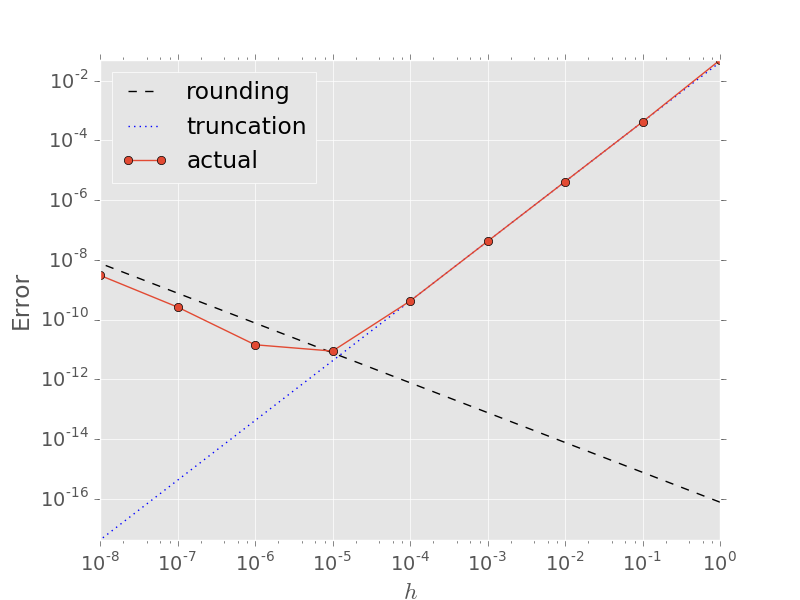
\includegraphics[width=0.6\linewidth,height=\textheight,keepaspectratio]{im/diffrounding.png}
\end{center}

You see that once \(h\) is small enough, rounding error takes over and
the error in the computed derivative starts to increase again.

\end{fbxSimple}

\subsection{Richardson extrapolation}\label{richardson-extrapolation}

Finding higher-order formulae by differentiating Lagrange polynomials is
tedious, and there is a simpler trick to obtain higher-order formulae,
called \textbf{Richardson extrapolation}.

We begin from the central-difference formula. Since we will use formulae
with different \(h\), let us define the notation \[
D_h := \frac{f(x_1+h) - f(x_1-h)}{2h}.
\]

Now use Taylor's theorem to expand more terms in the truncation error:
\[
\begin{aligned}
f(x_1 \pm h) = f(x_1) &\pm f'(x_1)h + \frac{f''(x_1)}{2}h^2 \pm \frac{f'''(x_1)}{3!}h^3 \\ &+ \frac{f^{(4)}(x_1)}{4!}h^4 \pm \frac{f^{(5)}(x_1)}{5!}h^5 + {\cal O}(h^6).
\end{aligned}
\] Substituting into the formula for \(D_h\), the even powers of \(h\)
cancel and we get \[
\begin{aligned}
D_h &= \frac{1}{2h}\Big(2f'(x_1)h + 2f'''(x_1)\frac{h^3}{6} +   2f^{(5)}(x_1)\frac{h^5}{120} + {\cal O}(h^7)  \Big)\\
&=f'(x_1) + f'''(x_1)\frac{h^2}{6} + f^{(5)}(x_1)\frac{h^4}{120} + {\cal O}(h^6).
\end{aligned}
\]

\begin{tcolorbox}[enhanced jigsaw, bottomrule=.15mm, colbacktitle=quarto-callout-note-color!10!white, breakable, arc=.35mm, coltitle=black, colback=white, bottomtitle=1mm, opacityback=0, title=\textcolor{quarto-callout-note-color}{\faInfo}\hspace{0.5em}{Note}, titlerule=0mm, toptitle=1mm, opacitybacktitle=0.6, colframe=quarto-callout-note-color-frame, leftrule=.75mm, rightrule=.15mm, left=2mm, toprule=.15mm]

You may not have seen the \textbf{big-Oh notation}. When we write
\(f(x) = {\cal O}(g(x))\), we mean \[
\lim_{x\to 0}\frac{|f(x)|}{|g(x)|} \leq M < \infty.
\] So the error is \({\cal O}(h^6)\) if it gets smaller at least as fast
as \(h^6\) as \(h\to 0\) (essentially, it contains no powers of \(h\)
less than 6).

\end{tcolorbox}

The leading term in the error here has the same coefficient \(h^2/6\) as
the truncation error we derived earlier, although we have now expanded
the error to higher powers of \(h\).

The trick is to apply the same formula with different step-sizes,
typically \(h\) and \(h/2\): \[
\begin{aligned}
D_h &= f'(x_1) + f'''(x_1)\frac{h^2}{6} + f^{(5)}(x_1)\frac{h^4}{120} + {\cal O}(h^6),\\
D_{h/2} &= f'(x_1) + f'''(x_1)\frac{h^2}{2^2(6)} + f^{(5)}(x_1)\frac{h^4}{2^4(120)} + {\cal O}(h^6).
\end{aligned}
\] We can then eliminate the \(h^2\) term by simple algebra: \[
\begin{aligned}
D_h - 2^2D_{h/2} =& -3f'(x_1) + \left(1 - \frac{2^2}{2^4}\right)f^{(5)}(x_1)\frac{h^4}{120} + {\cal O}(h^6),\\
\implies \quad D_h^{(1)} :=& \frac{2^2D_{h/2} - D_h}{3} = f'(x_1) - f^{(5)}(x_1)\frac{h^4}{480} + {\cal O}(h^6).
\end{aligned}
\] The new formula \(D_h^{(1)}\) is 4th-order accurate.

\phantomsection\label{derivative-of-fxlogx-at-x2-central-difference.}
\begin{fbxSimple}{eg}{Example 4.5: }{Derivative of \(f(x)=\log(x)\) at \(x=2\) (central difference).}
\phantomsection\label{derivative-of-fxlogx-at-x2-central-difference.}

\begin{longtable}[]{@{}
  >{\raggedright\arraybackslash}p{(\linewidth - 8\tabcolsep) * \real{0.1061}}
  >{\raggedright\arraybackslash}p{(\linewidth - 8\tabcolsep) * \real{0.2273}}
  >{\raggedright\arraybackslash}p{(\linewidth - 8\tabcolsep) * \real{0.2121}}
  >{\raggedright\arraybackslash}p{(\linewidth - 8\tabcolsep) * \real{0.2424}}
  >{\raggedright\arraybackslash}p{(\linewidth - 8\tabcolsep) * \real{0.2121}}@{}}
\toprule\noalign{}
\begin{minipage}[b]{\linewidth}\raggedright
\(h\)
\end{minipage} & \begin{minipage}[b]{\linewidth}\raggedright
\(D_h\)
\end{minipage} & \begin{minipage}[b]{\linewidth}\raggedright
Error
\end{minipage} & \begin{minipage}[b]{\linewidth}\raggedright
\(D_h^{(1)}\)
\end{minipage} & \begin{minipage}[b]{\linewidth}\raggedright
Error
\end{minipage} \\
\midrule\noalign{}
\endhead
\bottomrule\noalign{}
\endlastfoot
1.0 & 0.5493061443 & 0.04930614433 & 0.4979987836 & 0.00200121642 \\
0.1 & 0.5004172928 & 0.00041729278 & 0.4999998434 & 1.56599487e-07 \\
0.01 & 0.5000041667 & 4.16672916e-06 & 0.5000000000 & 1.56388791e-11 \\
0.001 & 0.5000000417 & 4.16666151e-08 & 0.5000000000 & 9.29256672e-14 \\
\end{longtable}

\end{fbxSimple}

In fact, we could have applied this \textbf{Richardson extrapolation}
procedure without knowing the coefficients of the error series. If we
have some general order-\(n\) approximation \[
D_h = f'(x) + Ch^n + {\cal O}(h^{n+1}),
\] then we can always evaluate it with \(h/2\) to get \[
D_{h/2} = f'(x) + C\frac{h^n}{2^n} + {\cal O}(h^{n+1})
\] and then eliminate the \(h^n\) term to get a new approximation \[
D_h^{(1)} := \frac{2^nD_{h/2} - D_h}{2^n - 1} = f'(x) + {\cal O}(h^{n+1}).
\]

\begin{tcolorbox}[enhanced jigsaw, bottomrule=.15mm, colbacktitle=quarto-callout-note-color!10!white, breakable, arc=.35mm, coltitle=black, colback=white, bottomtitle=1mm, opacityback=0, title=\textcolor{quarto-callout-note-color}{\faInfo}\hspace{0.5em}{Note}, titlerule=0mm, toptitle=1mm, opacitybacktitle=0.6, colframe=quarto-callout-note-color-frame, leftrule=.75mm, rightrule=.15mm, left=2mm, toprule=.15mm]

The technique is used not only in differentiation but also in
\textbf{Romberg integration} and the \textbf{Bulirsch-Stoer method} for
solving ODEs.

\end{tcolorbox}

\begin{tcolorbox}[enhanced jigsaw, bottomrule=.15mm, colbacktitle=quarto-callout-note-color!10!white, breakable, arc=.35mm, coltitle=black, colback=white, bottomtitle=1mm, opacityback=0, title=\textcolor{quarto-callout-note-color}{\faInfo}\hspace{0.5em}{Note}, titlerule=0mm, toptitle=1mm, opacitybacktitle=0.6, colframe=quarto-callout-note-color-frame, leftrule=.75mm, rightrule=.15mm, left=2mm, toprule=.15mm]

There is nothing special about taking \(h/2\); we could have taken
\(h/3\) or even \(2h\), and modified the formula accordingly. But
\(h/2\) is usually convenient.

\end{tcolorbox}

Furthermore, Richardson extrapolation can be applied iteratively. In
other words, we can now combine \(D_{h}^{(1)}\) and \(D_{h/2}^{(1)}\) to
get an even higher order approximation \(D_h^{(2)}\), and so on.

\phantomsection\label{iterated-richardson-extrapolation-for-central-differences.}
\begin{fbxSimple}{eg}{Example 4.6: }{Iterated Richardson extrapolation for central differences.}
\phantomsection\label{iterated-richardson-extrapolation-for-central-differences.}
From \[
\begin{aligned}
D_h^{(1)} &= f'(x_1) + C_1h^4 + {\cal O}(h^6),\\
D_{h/2}^{(1)} &= f'(x_1) + C_1\frac{h^4}{2^4} + {\cal O}(h^6),
\end{aligned}
\] we can eliminate the \(h^4\) term to get the 6th-order approximation
\[
D_h^{(2)} := \frac{2^4D_{h/2}^{(1)} - D_h^{(1)}}{2^4 - 1}.
\]

\end{fbxSimple}

\begin{tcolorbox}[enhanced jigsaw, bottomrule=.15mm, colbacktitle=quarto-callout-note-color!10!white, breakable, arc=.35mm, coltitle=black, colback=white, bottomtitle=1mm, opacityback=0, title=\textcolor{quarto-callout-note-color}{\faInfo}\hspace{0.5em}{Note}, titlerule=0mm, toptitle=1mm, opacitybacktitle=0.6, colframe=quarto-callout-note-color-frame, leftrule=.75mm, rightrule=.15mm, left=2mm, toprule=.15mm]

Lewis Fry Richardson (1881--1953) was from Newcastle and an
undergraduate there (when it was still a College of Durham). He was the
first person to apply mathematics (finite differences) to weather
prediction, and was ahead of his time: in the absence of electronic
computers, he estimated that 60,000 people would be needed to predict
the next day's weather!

\end{tcolorbox}

\section{Numerical integration}\label{s-int}

\begin{quote}
\emph{How do we calculate integrals numerically?}
\end{quote}

The definite integral \[
I(f) := \int_a^b f(x)\,\mathrm{d}x
\] can usually not be evaluated in closed form. To approximate it
numerically, we can use a \textbf{quadrature formula} \[
I_n(f) := \sum_{k=0}^n \sigma_k f(x_k),
\] where \(x_0,\ldots,x_n\) are a set of \textbf{nodes} and
\(\sigma_0,\ldots,\sigma_n\) are a set of corresponding
\textbf{weights}.

\begin{tcolorbox}[enhanced jigsaw, bottomrule=.15mm, colbacktitle=quarto-callout-note-color!10!white, breakable, arc=.35mm, coltitle=black, colback=white, bottomtitle=1mm, opacityback=0, title=\textcolor{quarto-callout-note-color}{\faInfo}\hspace{0.5em}{Note}, titlerule=0mm, toptitle=1mm, opacitybacktitle=0.6, colframe=quarto-callout-note-color-frame, leftrule=.75mm, rightrule=.15mm, left=2mm, toprule=.15mm]

The nodes are also known as \textbf{quadrature points} or
\textbf{abscissas}, and the weights as \textbf{coefficients}.

\end{tcolorbox}

\phantomsection\label{the-trapezium-rule}
\begin{fbxSimple}{eg}{Example 4.7: }{The trapezium rule}
\phantomsection\label{the-trapezium-rule}
\[
I_1(f) = \frac{b-a}{2}\Big( f(a) + f(b) \Big).
\]

This is the quadrature formula above with \(x_0=a\), \(x_1=b\),
\(\sigma_0=\sigma_1=\tfrac12(b-a)\).

For example, with \(a=0\), \(b=2\), \(f(x)=\mathrm{e}^x\), we get \[
I_1(f) = \frac{2 - 0}{2}\big(\mathrm{e}^0 + \mathrm{e}^{2}\big) = 8.389 \quad \textrm{to 4 s.f.}
\] The exact answer is \[
I(f) = \int_0^{2}\mathrm{e}^x\,\mathrm{d}x = \mathrm{e}^{2} - \mathrm{e}^0 = 6.389 \quad \textrm{to 4 s.f.}
\] Graphically, \(I_1(f)\) measures the area under the straight line
that interpolates \(f\) at the ends:

\begin{center}
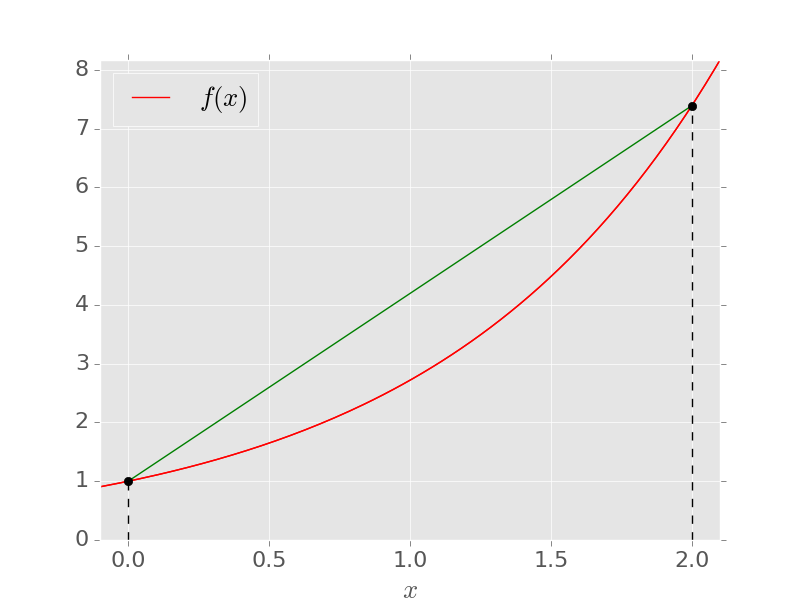
\includegraphics[width=0.6\linewidth,height=\textheight,keepaspectratio]{im/trapz.png}
\end{center}

\end{fbxSimple}

\subsection{Newton-Cotes formulae}\label{newton-cotes-formulae}

We can derive a family of ``interpolatory'' quadrature formulae by
integrating interpolating polynomials of different degrees. We will also
get error estimates using the interpolation error theorem.

Let \(x_0, \ldots, x_n \in [a,b]\), where \(x_0 < x_1 < \cdots < x_n\),
be a set of \(n+1\) nodes, and let \(p_n\in{\cal P}_n\) be the
polynomial that interpolates \(f\) at these nodes. This may be written
in Lagrange form as \[
p_n(x) = \sum_{k=0}^n f(x_k)\ell_k(x), \quad \textrm{where}\quad \ell_k(x) = \prod_{\substack{j=0\\j\neq k}}^n\frac{x - x_j}{x_k - x_j}.
\] To approximate \(I(f)\), we integrate \(p_n(x)\) to define the
quadrature formula \[
I_n(f) := \int_a^b\sum_{k=0}^n f(x_k)\ell_k(x)\,\mathrm{d}x = \sum_{k=0}^n f(x_k)\int_a^b\ell_k(x)\,\mathrm{d}x.
\] In other words, \[
I_n(f) := \sum_{k=0}^n\sigma_k f(x_k), \quad \textrm{where} \quad \sigma_k = \int_a^b\ell_k(x)\,\mathrm{d}x.
\] When the nodes are equidistant, this is called a \textbf{Newton-Cotes
formula}. If \(x_0=a\) and \(x_n=b\), it is called a \textbf{closed
Newton-Cotes formula}.

\begin{tcolorbox}[enhanced jigsaw, bottomrule=.15mm, colbacktitle=quarto-callout-note-color!10!white, breakable, arc=.35mm, coltitle=black, colback=white, bottomtitle=1mm, opacityback=0, title=\textcolor{quarto-callout-note-color}{\faInfo}\hspace{0.5em}{Note}, titlerule=0mm, toptitle=1mm, opacitybacktitle=0.6, colframe=quarto-callout-note-color-frame, leftrule=.75mm, rightrule=.15mm, left=2mm, toprule=.15mm]

An \textbf{open Newton-Cotes formula} has nodes \(x_i = a + (i+1)h\) for
\(h = (b-a)/(n+2)\).

\end{tcolorbox}

\phantomsection\label{trapezium-rule}
\begin{fbxSimple}{eg}{Example 4.8: }{Trapezium rule}
\phantomsection\label{trapezium-rule}
This is the closed Newton-Cotes formula with \(n=1\). To see this, let
\(x_0=a\), \(x_1=b\). Then \[
\begin{aligned}
\ell_0(x) = \frac{x-b}{a-b} \implies \sigma_0 &= \int_a^b\ell_0(x)\,\mathrm{d}x \\ &= \frac{1}{a-b}\int_a^b(x-b)\,\mathrm{d}x \\ &= \frac{1}{2(a-b)}(x-b)^2\big|_a^b \\ &= \frac{b-a}{2},
\end{aligned}
\] and \[
\begin{aligned}
\ell_1(x) = \frac{x-a}{b-a} \implies \sigma_1 &= \int_a^b\ell_1(x)\,\mathrm{d}x \\ &= \frac{1}{b-a}\int_a^b(x-a)\,\mathrm{d}x \\ &= \frac{1}{2(b-a)}(x-a)^2\big|_a^b = \frac{b-a}{2}.
\end{aligned}
\] This gives \[
I_1(f) = \sigma_0f(a) + \sigma_1f(b) = \frac{b-a}{2}\big(f(a) + f(b)\big).
\]

\end{fbxSimple}

\phantomsection\label{theorem-4.1}
\begin{fbxSimple}{theorem}{Theorem 4.1}{}
\phantomsection\label{theorem-4.1}
Let \(f\) be continuous on \([a,b]\) with \(n+1\) continuous derivatives
on \((a,b)\). Then the Newton-Cotes formula above satisfies the error
bound \[
\begin{aligned}
&\big|I(f) - I_n(f)\big| \leq \\ &\frac{\max_{\xi\in[a,b]}|f^{(n+1)}(\xi)|}{(n+1)!}\int_a^b\big|(x-x_0)(x-x_1)\cdots(x-x_{n}) \big|\,\mathrm{d}x.
\end{aligned}
\]

\end{fbxSimple}

\textbf{Proof:}\\
First note that the error in the Newton-Cotes formula may be written \[
\begin{aligned}
\big|I(f) - I_n(f)\big| &= \left|\int_a^bf(x)\,\mathrm{d}x - \int_a^bp_n(x)\,\mathrm{d}x \right| \\
&= \left| \int_a^b\big[f(x) - p_n(x)\big]\,\mathrm{d}x\right| \\
&\leq \int_a^b\big|f(x) - p_n(x)\big|\,\mathrm{d}x.
\end{aligned}
\] Now recall the interpolation error theorem, which says that, for each
\(x\in[a,b]\), we can write \[
f(x) - p_n(x) = \frac{f^{(n+1)}(\xi)}{(n+1)!}(x-x_0)(x-x_1)\cdots(x-x_{n})
\] for some \(\xi\in(a,b)\). The theorem simply follows by inserting
this into the inequality above. \(\Box\)

\phantomsection\label{trapezium-rule-error}
\begin{fbxSimple}{eg}{Example 4.9: }{Trapezium rule error}
\phantomsection\label{trapezium-rule-error}
Let \(M_2 = \max_{\xi\in[a,b]}|f''(\xi)|\). Here the theorem reduces to
\[
\begin{aligned}
\big|I(f) - I_1(f)\big| &\leq \frac{M_2}{(1+1)!}\int_a^b\big|(x-a)(x-b)\big|\,\mathrm{d}x \\ &= \frac{M_2}{2!}\int_a^b(x-a)(b-x)\,\mathrm{d}x \\ &= \frac{(b-a)^3}{12}M_2.
\end{aligned}
\] For our earlier example with \(a=0\), \(b=2\), \(f(x)=\mathrm{e}^x\),
the estimate gives \[
\big|I(f) - I_1(f)\big| \leq \tfrac1{12}(2^3)\mathrm{e}^{2} \approx 4.926.
\] This is an overestimate of the actual error which was
\(\approx 2.000\).

\end{fbxSimple}

The theorem suggests that the accuracy of \(I_n\) is limited both by the
smoothness of \(f\) (outside our control) and by the location of the
nodes \(x_k\). If the nodes are free to be chosen, then we can use
\textbf{Gaussian integration} (more to follow on that topic).

\begin{tcolorbox}[enhanced jigsaw, bottomrule=.15mm, colbacktitle=quarto-callout-note-color!10!white, breakable, arc=.35mm, coltitle=black, colback=white, bottomtitle=1mm, opacityback=0, title=\textcolor{quarto-callout-note-color}{\faInfo}\hspace{0.5em}{Note}, titlerule=0mm, toptitle=1mm, opacitybacktitle=0.6, colframe=quarto-callout-note-color-frame, leftrule=.75mm, rightrule=.15mm, left=2mm, toprule=.15mm]

As with interpolation, taking a high \(n\) is not usually a good idea.
One can prove for the closed Newton-Cotes formula that \[
\sum_{k=0}^n|\sigma_k| \to \infty \quad \textrm{as} \quad n\to\infty.
\] This makes the quadrature vulnerable to rounding errors for large
\(n\).

\end{tcolorbox}

\subsection{Composite Newton-Cotes
formulae}\label{composite-newton-cotes-formulae}

Since the Newton-Cotes formulae are based on polynomial interpolation at
equally-spaced points, the results do not converge as the number of
nodes increases. A better way to improve accuracy is to divide the
interval \([a,b]\) into \(m\) subintervals \([x_{i-1},x_i]\) of equal
length \[
h := \frac{b-a}{m},
\] and use a Newton-Cotes formula of small degree \(n\) on each
subinterval.

\phantomsection\label{composite-trapezium-rule}
\begin{fbxSimple}{eg}{Example 4.10: }{Composite trapezium rule}
\phantomsection\label{composite-trapezium-rule}
Applying the trapezium rule \(I_1(f)\) on each subinterval gives \[
\begin{aligned}
C_{1,m}(f) &= \frac{h}{2}\left[f(x_0) + f(x_1) + f(x_1) + f(x_2) + \ldots + f(x_{m-1}) + f(x_m) \right],\\
&= h\left[\tfrac12 f(x_0) + f(x_1) + f(x_2) + \ldots + f(x_{m-1}) + \tfrac12 f(x_m) \right].
\end{aligned}
\] We are effectively integrating a piecewise-linear approximation of
\(f(x)\); here we show \(m=3\) for our test problem
\(f(x)=\mathrm{e}^x\) on \([0,2]\):

\begin{center}
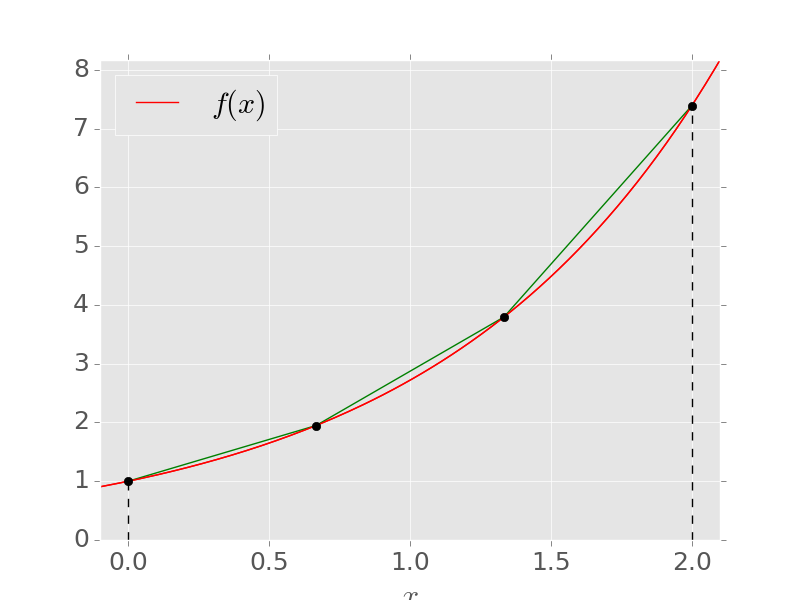
\includegraphics[width=0.75\linewidth,height=\textheight,keepaspectratio]{im/comptrapz.png}
\end{center}

Look at what happens as we increase \(m\) for our test problem:

\begin{longtable}[]{@{}llll@{}}
\toprule\noalign{}
\(m\) & \(h\) & \(C_{1,m}(f)\) & \(|I(f) - C_{1,m}(f)|\) \\
\midrule\noalign{}
\endhead
\bottomrule\noalign{}
\endlastfoot
1 & 2 & 8.389 & 2.000 \\
2 & 1 & 6.912 & 0.524 \\
4 & 0.5 & 6.522 & 0.133 \\
8 & 0.25 & 6.422 & 0.033 \\
16 & 0.125 & 6.397 & 0.008 \\
32 & 0.0625 & 6.391 & 0.002 \\
\end{longtable}

When we halve the sub-interval \(h\), the error goes down by a factor
\(4\), suggesting that we have quadratic convergence, i.e.,
\({\cal O}(h^2)\).

To show this theoretically, we can apply the Newton-Cotes error theorem
in each subinterval. In \([x_{i-1},x_i]\) we have \[
\big|I(f) - I_1(f)\big| \leq \frac{\max_{\xi\in[x_{i-1},x_i]}|f''(\xi)|}{2!}\int_{x_{i-1}}^{x_i}\big|(x-x_{i-1})(x-x_i)\big|\,\mathrm{d}x
\] Note that \[
\begin{aligned}
\int_{x_{i-1}}^{x_i}\big|(x-x_{i-1})(x-x_i)\big|\,\mathrm{d}x &= \int_{x_{i-1}}^{x_i}(x-x_{i-1})(x_i-x)\,\mathrm{d}x \\
&= \int_{x_{i-1}}^{x_i}\big[-x^2 + (x_{i-1} + x_i)x - x_{i-1}x_i\big]\,\mathrm{d}x\\
&= \big[-\tfrac13x^3 + \tfrac12(x_{i-1}+x_i)x^2 - x_{i-1}x_ix\big]_{x_{i-1}}^{x_i} \\
&= \tfrac16 x_{i}^3 - \tfrac12x_{i-1}x_i^2 + \tfrac12x_{i-1}^2x_i - \tfrac16x_{i-1}^3\\
&= \tfrac16(x_i - x_{i-1})^3 = \tfrac16 h^3.
\end{aligned}
\] So overall \[
\begin{aligned}
\big| I(f) - C_{1,m}(f) \big| &\leq \tfrac12 \max_i\left(\max_{\xi\in[x_{i-1},x_i]}|f''(\xi)|\right) m\frac{h^3}{6}\\
  &= \frac{mh^3}{12}\max_{\xi\in[a,b]}|f''(\xi)| =  \frac{b-a}{12}h^2\max_{\xi\in[a,b]}|f''(\xi)|.
 \end{aligned}
\] As long as \(f\) is sufficiently smooth, this shows that the
composite trapezium rule will converge as \(m\to\infty\). Moreover, the
convergence will be \({\cal O}(h^2)\).

\end{fbxSimple}

\subsection{Exactness}\label{exactness}

From the Newton-Cotes error theorem, we see that the Newton-Cotes
formula \(I_n(f)\) will give the exact answer if \(f^{(n+1)}=0\). In
other words, it will be exact if \(f \in{\cal P}_n\).

\phantomsection\label{eg-4.11}
\begin{fbxSimple}{eg}{Example 4.11}{}
\phantomsection\label{eg-4.11}
The trapezium rule \(I_1(f)\) is exact for all linear polynomials
\(f\in{\cal P}_1\).

\end{fbxSimple}

The \textbf{degree of exactness} of a quadrature formula is the largest
integer \(n\) for which the formula is exact for all polynomials in
\({\cal P}_n\).

To check whether a quadrature formula has degree of exactness \(n\), it
suffices to check whether it is exact for the basis \(1\), \(x\),
\(x^2, \ldots, x^n\).

\phantomsection\label{simpsons-rule}
\begin{fbxSimple}{eg}{Example 4.12: }{Simpson’s rule}
\phantomsection\label{simpsons-rule}
This is the \(n=2\) closed Newton-Cotes formula \[
I_2(f) = \frac{b-a}{6}\left[f(a) + 4f\left(\frac{a+b}{2}\right) + f(b)\right],
\] derived by integrating a quadratic interpolating polynomial. Let us
find its degree of exactness: \[
\begin{aligned}
I(1) &= \int_a^b\,\mathrm{d}x = (b-a), \\
I_2(1) &= \frac{b-a}{6}[1 + 4 + 1] = b-a = I(1),\\
I(x) &= \int_a^b x\,\mathrm{d}x = \frac{b^2-a^2}{2}, \\
I_2(x) &= \frac{b-a}{6}\left[a + 2(a+b) + b\right] = \frac{(b-a)(b+a)}{2} = I(x),\\
I(x^2) &= \int_a^b x^2\,\mathrm{d}x = \frac{b^3 - a^3}{3}, \\
I_2(x^2) &= \frac{b-a}{6}\left[a^2 + (a+b)^2 + b^2\right] = \frac{2(b^3 - a^3)}{6} = I(x^2),\\
I(x^3) &= \int_a^b x^3\,\mathrm{d}x = \frac{b^4 - a^4}{4}, \\
I_2(x^3) &= \frac{b-a}{6}\left[a^3 + \tfrac12(a+b)^3 + b^3 \right] = \frac{b^4-a^4}{4} = I(x^3).
\end{aligned}
\] This shows that the degree of exactness is at least 3 (contrary to
what might be expected from the interpolation picture). You can verify
that \(I_2(x^4)\neq I(x^4)\), so the degree of exactness is exactly 3.

\end{fbxSimple}

This shows that the term \(f'''(\xi)\) in the error formula for
Simpson's rule is misleading. In fact, it is possible to write an error
bound proportional to \(f^{(4)}(\xi)\).

In terms of degree of exactness, Simpson's formula does better than
expected. In general, Newton-Cotes formulae with even \(n\) have degree
of exactness \(n+1\). But this is by no means the highest possible (see
next section).

\subsection{Gaussian quadrature}\label{gaussian-quadrature}

The idea of \textbf{Gaussian quadrature} is to choose not only the
weights \(\sigma_k\) but also the nodes \(x_k\), in order to achieve the
highest possible degree of exactness.

Firstly, we will illustrate the brute force \textbf{method of
undetermined coefficients}.

\phantomsection\label{gaussian-quadrature-formula-g_1fsum_k01sigma_kfx_k-on-the-interval--11}
\begin{fbxSimple}{eg}{Example 4.13: }{Gaussian quadrature formula \(G_1(f)=\sum_{k=0}^1\sigma_kf(x_k)\) on the interval \([-1,1]\)}
\phantomsection\label{gaussian-quadrature-formula-g_1fsum_k01sigma_kfx_k-on-the-interval--11}
Here we have four unknowns \(x_0\), \(x_1\), \(\sigma_0\) and
\(\sigma_1\), so we can impose four conditions: \[
\begin{aligned}
G_1(1) &= I(1) \implies \sigma_0 + \sigma_1 = \int_{-1}^1\,\mathrm{d}x = 2,\\
G_1(x) &= I(x) \implies \sigma_0x_0 + \sigma_1x_1 = \int_{-1}^1x\,\mathrm{d}x = 0,\\
G_1(x^2) &= I(x^2) \implies \sigma_0x_0^2 + \sigma_1x_1^2 = \int_{-1}^1x^2\,\mathrm{d}x = \tfrac23,\\
G_1(x^3) &= I(x^3) \implies \sigma_0x_0^3 + \sigma_1x_1^3 = \int_{-1}^1x^3\,\mathrm{d}x = 0.
\end{aligned}
\] To solve this system, the symmetry suggests that \(x_1=-x_0\) and
\(\sigma_0=\sigma_1\). This will automatically satisfy the equations for
\(x\) and \(x^3\), leaving the two equations \[
2\sigma_0 = 2, \qquad 2\sigma_0x_0^2 = \tfrac23,
\] so that \(\sigma_0=\sigma_1=1\) and \(x_1=-x_0 = 1/\sqrt{3}\). The
resulting Gaussian quadrature formula is \[
G_1(f) = f\left(-\frac{1}{\sqrt{3}}\right) + f\left(\frac{1}{\sqrt{3}}\right).
\] This formula has degree of exactness 3.

\end{fbxSimple}

In general, the Gaussian quadrature formula with \(n\) nodes will have
degree of exactness \(2n+1\).

The method of undetermined coefficients becomes unworkable for larger
numbers of nodes, because of the nonlinearity of the equations. A much
more elegant method uses orthogonal polynomials. In addition to what we
learned before, we will need the following result.

\phantomsection\label{theorem-4.2}
\begin{fbxSimple}{theorem}{Theorem 4.2}{}
\phantomsection\label{theorem-4.2}
If \(\{\phi_0,\phi_1,\ldots,\phi_n\}\) is a set of orthogonal
polynomials on \([a,b]\) under the inner product
\((f,g) = \int_a^b f(x)g(x)w(x)\,\mathrm{d}x\) and \(\phi_k\) is of
degree \(k\) for each \(k=0,1,\ldots,n\), then \(\phi_k\) has \(k\)
distinct real roots, and these roots lie in the interval \([a,b]\).

\end{fbxSimple}

\textbf{Proof:}\\
Let \(x_1,\ldots,x_j\) be the points where \(\phi_k(x)\) changes sign in
\([a,b]\). If \(j=k\) then we are done. Otherwise, suppose \(j<k\), and
consider the polynomial \[
q_j(x) = (x-x_1)(x-x_2)\cdots(x-x_j).
\] Since \(q_j\) has lower degree than \(\phi_k\), they must be
orthogonal, meaning \[
(q_j,\phi_k)=0 \implies \int_a^b q_j(x)\phi_k(x)w(x)\,\mathrm{d}x = 0.
\] On the other hand, notice that the product \(q_j(x)\phi_k(x)\) cannot
change sign in \([a,b]\), because each sign change in \(\phi_k(x)\) is
cancelled out by one in \(q_j(x)\). This means that \[
\int_a^b q_j(x)\phi_k(x)w(x)\,\mathrm{d}x \neq 0,
\] which is a contradiction. \(\Box\)

Remarkably, these roots are precisely the optimum choice of nodes for a
quadrature formula to approximate the (weighted) integral \[
I_{w}(f) = \int_a^b f(x)w(x)\,\mathrm{d}x.
\]

\phantomsection\label{gaussian-quadrature-1}
\begin{fbxSimple}{theorem}{Theorem 4.3: }{Gaussian quadrature}
\phantomsection\label{gaussian-quadrature-1}
Let \(\phi_{n+1}\) be a polynomial in \({\cal P}_{n+1}\) that is
orthogonal on \([a,b]\) to all polynomials in \({\cal P}_{n}\), with
respect to the weight function \(w(x)\). If \(x_0,x_1,\ldots,x_n\) are
the roots of \(\phi_{n+1}\), then the quadrature formula \[
G_{n,w}(f) := \sum_{k=0}^n\sigma_kf(x_k), \qquad \sigma_k = \int_a^b\ell_k(x)w(x)\,\mathrm{d}x
\] approximates \(I_w(f)\) with degree of exactness \({2n+1}\) (the
largest possible).

\end{fbxSimple}

Like Newton-Cotes, we see that Gaussian quadrature is based on
integrating an interpolating polynomial, but now the nodes are the roots
of an orthogonal polynomial, rather than equally spaced points.

\phantomsection\label{gaussian-quadrature-with-n1-on--11-and-wx1-again}
\begin{fbxSimple}{eg}{Example 4.14: }{Gaussian quadrature with \(n=1\) on \([-1,1]\) and \(w(x)=1\) (again)}
\phantomsection\label{gaussian-quadrature-with-n1-on--11-and-wx1-again}
To find the nodes \(x_0\), \(x_1\), we need to find the roots of the
orthogonal polynomial \(\phi_2(x)\). For this inner product, we already
computed this (Legendre polynomial) in Chapter 3, where we found \[
\phi_2(x) = x^2 - \tfrac13.
\] Thus the nodes are \(x_0= -1/\sqrt{3}, x_1=1/\sqrt{3}\). Integrating
the Lagrange polynomials gives the corresponding weights \[
\begin{aligned}
\sigma_0 &= \int_{-1}^1\ell_0(x)\,\mathrm{d}x = \int_{-1}^1\frac{x-\tfrac1{\sqrt{3}}}{-\tfrac2{\sqrt{3}}}\,\mathrm{d}x = -\tfrac{\sqrt{3}}{2}\left[\tfrac12x^2 - \tfrac1{\sqrt{3}}x\right]_{-1}^1 = 1,\\
\sigma_1 &= \int_{-1}^1\ell_1(x)\,\mathrm{d}x = \int_{-1}^1\frac{x+\tfrac1{\sqrt{3}}}{\tfrac2{\sqrt{3}}}\,\mathrm{d}x = \tfrac{\sqrt{3}}{2}\left[\tfrac12x^2 + \tfrac1{\sqrt{3}}x\right]_{-1}^1 = 1,
\end{aligned}
\] as before.

\end{fbxSimple}

\begin{tcolorbox}[enhanced jigsaw, bottomrule=.15mm, colbacktitle=quarto-callout-note-color!10!white, breakable, arc=.35mm, coltitle=black, colback=white, bottomtitle=1mm, opacityback=0, title=\textcolor{quarto-callout-note-color}{\faInfo}\hspace{0.5em}{Note}, titlerule=0mm, toptitle=1mm, opacitybacktitle=0.6, colframe=quarto-callout-note-color-frame, leftrule=.75mm, rightrule=.15mm, left=2mm, toprule=.15mm]

Using an appropriate weight function \(w(x)\) can be useful for
integrands with a singularity, since we can incorporate this in \(w(x)\)
and still approximate the integral with \(G_{n,w}\).

\end{tcolorbox}

\phantomsection\label{gaussian-quadrature-for-int_01-cosxx-12mathrmdx-with-n0}
\begin{fbxSimple}{eg}{Example 4.15: }{Gaussian quadrature for \(\int_0^1 \cos(x)x^{-1/2}\,\mathrm{d}x\), with \(n=0\)}
\phantomsection\label{gaussian-quadrature-for-int_01-cosxx-12mathrmdx-with-n0}

This is a Fresnel integral, with exact value \(1.80905\ldots\) Let us
compare the effect of using an appropriate weight function.

\begin{enumerate}
\def\labelenumi{\arabic{enumi}.}
\item
  \emph{Unweighted quadrature (\(w(x)\equiv 1\)).} The orthogonal
  polynomial of degree 1 is \[
  \phi_1(x) = x - \frac{\int_0^1x\,\mathrm{d}x}{\int_0^1\,\mathrm{d}x} = x-\tfrac12 \implies x_0=\tfrac12.
  \] The corresponding weight may be found by imposing
  \(G_{0}(1)=I(1)\), which gives \(\sigma_0=\int_0^1\,\mathrm{d}x = 1\).
  Then our estimate is \[
  G_0\left(\frac{\cos(x)}{\sqrt{x}}\right) = \frac{\cos\left(\tfrac12\right)}{\sqrt{\tfrac12}} = 1.2411\ldots
  \]
\item
  \emph{Weighted quadrature with \(w(x) = x^{-1/2}\).} This time we get
  \[
  \phi_1(x) = x - \frac{\int_0^1x^{1/2}\,\mathrm{d}x}{\int_0^1x^{-1/2}\,\mathrm{d}x} = x-\frac{2/3}{2} \implies x_0=\tfrac13.
  \] The corresponding weight is
  \(\sigma_0 = \int_0^1x^{-1/2}\,\mathrm{d}x = 2\), so the new estimate
  is the more accurate \[
  G_{0,w}\big(\cos(x)\big) = 2\cos\left(\tfrac13\right) = 1.8899\ldots
  \]
\end{enumerate}

\end{fbxSimple}

\textbf{Proof:}

First, recall that any interpolatory quadrature formula based on \(n+1\)
nodes will be exact for all polynomials in \({\cal P}_n\) (this follows
from the Newton-Cotes theorem, which can be modified to include the
weight function \(w(x)\)). So in particular, \(G_{n,w}\) is exact for
\(p_n\in{\cal P}_n\).

Now let \(p_{2n+1}\in{\cal P}_{2n+1}\). The trick is to divide this by
the orthogonal polynomial \(\phi_{n+1}\) whose roots are the nodes. This
gives \[
p_{2n+1}(x) = \phi_{n+1}(x)q_n(x) + r_n(x) \quad \textrm{for some} \quad q_n,r_n \in{\cal P}_n.
\] Then \[
\begin{aligned}
G_{n,w}(p_{2n+1}) &= \sum_{k=0}^n\sigma_kp_{2n+1}(x_k) = \sum_{k=0}^n\sigma_k\Big[\phi_{n+1}(x_k)q_n(x_k) + r_n(x_k) \Big] \\ &= \sum_{k=0}^n\sigma_kr_n(x_k) = I_w(r_n),
\end{aligned}
\] where we have used the fact that \(G_{n,w}\) is exact for
\(r_n\in{\cal P}_n\). Now, since \(q_n\) has lower degree than
\(\phi_{n+1}\), it must be orthogonal to \(\phi_{n+1}\), so \[
I_w(\phi_{n+1}q_n) = \int_a^b\phi_{n+1}(x)q_n(x)w(x)\,\mathrm{d}x = 0
\] and hence \[
\begin{aligned}
G_{n,w}(p_{2n+1}) &= I_w(r_n) + 0= I_w(r_n) + I_w(\phi_{n+1}q_n) \\ &= I_w( \phi_{n+1}q_n + r_n) = I_w(p_{2n+1}).
\end{aligned}
\]

Unlike Newton-Cotes formulae with equally-spaced points, it can be shown
that \(G_{n,w}(f)\to I_w(f)\) as \(n\to\infty\), for any continuous
function \(f\). This follows (with a bit of analysis) from the fact that
all of the weights \(\sigma_k\) are positive, along with the fact that
they sum to a fixed number \(\int_a^bw(x)\,\mathrm{d}x\). For
Newton-Cotes, the signed weights still sum to a fixed number, but
\(\sum_{k=0}^n|\sigma_k|\to\infty\), which destroys convergence.

Not surprisingly, we can derive an error formula that depends on
\(f^{(2n+2)}(\xi)\) for some \(\xi\in(a,b)\). To do this, we will need
the following result from calculus.

\phantomsection\label{mean-value-theorem-for-integrals}
\begin{fbxSimple}{theorem}{Theorem 4.4: }{Mean value theorem for integrals}
\phantomsection\label{mean-value-theorem-for-integrals}
If \(f,g\) are continuous on \([a,b]\) and \(g(x)\geq 0\) for all
\(x\in[a,b]\), then there exists \(\xi\in(a,b)\) such that \[
\int_a^bf(x)g(x)\,\mathrm{d}x = f(\xi)\int_a^bg(x)\,\mathrm{d}x.
\]

\end{fbxSimple}

\textbf{Proof:}\\
Let \(m\) and \(M\) be the minimum and maximum values of \(f\) on
\([a,b]\), respectively. Since \(g(x)\geq 0\), we have that \[
m\int_a^bg(x)\,\mathrm{d}x \leq \int_a^bf(x)g(x)\,\mathrm{d}x \leq M\int_a^bg(x)\,\mathrm{d}x.
\] Now let \(I=\int_a^bg(x)\,\mathrm{d}x\). If \(I=0\) then
\(g(x)\equiv 0\), so \(\int_a^bf(x)g(x)\,\mathrm{d}x=0\) and the theorem
holds for every \(\xi\in(a,b)\). Otherwise, we have \[
m \leq \frac{1}{I}\int_a^bf(x)g(x)\,\mathrm{d}x \leq M.
\] By the Intermediate Value Theorem, \(f(x)\) attains every value
between \(m\) and \(M\) somewhere in \((a,b)\), so in particular there
exists \(\xi\in(a,b)\) with \[
f(\xi) = \frac{1}{I}\int_a^bf(x)g(x)\,\mathrm{d}x.
\]

\phantomsection\label{error-estimate-for-gaussian-quadrature}
\begin{fbxSimple}{theorem}{Theorem 4.5: }{Error estimate for Gaussian quadrature}
\phantomsection\label{error-estimate-for-gaussian-quadrature}
Let \(\phi_{n+1}\in{\cal P}_{n+1}\) be monic and orthogonal on \([a,b]\)
to all polynomials in \({\cal P}_n\), with respect to the weight
function \(w(x)\). Let \(x_0,x_1,\ldots,x_n\) be the roots of
\(\phi_{n+1}\), and let \(G_{n,w}(f)\) be the Gaussian quadrature
formula defined above. If \(f\) has \(2n+2\) continuous derivatives on
\((a,b)\), then there exists \(\xi\in(a,b)\) such that \[
I_w(f) - G_{n,w}(f) = \frac{f^{(2n+2)}(\xi)}{(2n+2)!}\int_a^b\phi_{n+1}^2(x)w(x)\,\mathrm{d}x.
\]

\end{fbxSimple}

\textbf{Proof:}\\
A neat trick is to use Hermite interpolation. Since the \(x_k\) are
distinct, there exists a unique polynomial \(p_{2n+1}\) such that \[
p_{2n+1}(x_k) = f(x_k), \quad p_{2n+1}'(x_k) = f'(x_k) \quad \textrm{for $k=0,\ldots,n$}.
\] In addition (see problem sheet), there exists \(\lambda\in(a,b)\),
depending on \(x\), such that \[
f(x) - p_{2n+1}(x) = \frac{f^{(2n+2)}(\lambda)}{(2n+2)!}\prod_{i=0}^n(x-x_i)^2.
\] Now we know that \((x-x_0)(x-x_1)\cdots(x-x_n)=\phi_{n+1}(x)\), since
we fixed \(\phi_{n+1}\) to be monic. Hence \[
\int_a^bf(x)w(x)\,\mathrm{d}x - \int_a^bp_{2n+1}(x)w(x)\,\mathrm{d}x = \int_a^b\frac{f^{(2n+2)}(\lambda)}{(2n+2)!}\phi_{n+1}^2(x)w(x)\,\mathrm{d}x.
\] Now we know that \(G_{n,w}\) must be exact for \(p_{2n+1}\), so \[
\int_a^bp_{2n+1}(x)w(x)\,\mathrm{d}x = G_{n,w}(p_{2n+1}) = \sum_{k=0}^n\sigma_kp_{2n+1}(x_k) = \sum_{k=0}^n\sigma_kf(x_k)=G_{n,w}(f).
\] For the right-hand side, we can't take \(f^{(2n+2)}(\lambda)\)
outside the integral since \(\lambda\) depends on \(x\). But
\(\phi_{n+1}^2(x)w(x)\geq 0\) on \([a,b]\), so we can apply the mean
value theorem for integrals and get \[
I_w(f) - G_{n,w}(f) = \frac{f^{(2n+2)}(\xi)}{(2n+2)!}\int_a^b\phi_{n+1}^2(x)w(x)\,\mathrm{d}x
\] for some \(\xi\in(a,b)\) that does not depend on \(x\).

\bookmarksetup{startatroot}

\chapter{Differential Equations}\label{differential-equations}

\begin{quote}
\emph{How can computers solve differential equations?}
\end{quote}

Almost all differential equations which arise in mathematics and its
applications do not have exact analytical solutions. This is a central
motivation for numerical analysis, as well as the historical development
of increasingly powerful computers. Most scientific computing languages
have pre-built packages for solving differential equations quickly and
accurately using numerical approximations, and there are entire classes
of software packages designed to do this for specialised industries,
such as aerospace or finance. The goal of this Chapter is to understand
the fundamentals of numerical timestepping, so that you can understand
properties of these numerical methods, and hence so you can choose which
to use for a given problem.

\begin{tcolorbox}[enhanced jigsaw, bottomrule=.15mm, colbacktitle=quarto-callout-note-color!10!white, breakable, arc=.35mm, coltitle=black, colback=white, bottomtitle=1mm, opacityback=0, title=\textcolor{quarto-callout-note-color}{\faInfo}\hspace{0.5em}{Note}, titlerule=0mm, toptitle=1mm, opacitybacktitle=0.6, colframe=quarto-callout-note-color-frame, leftrule=.75mm, rightrule=.15mm, left=2mm, toprule=.15mm]

This topic is vast, with many textbooks detailing aspects of numerical
differential equations from a variety of theoretical or applied
perspectives. We will focus on building up the mathematical terminology
of different classes of solvers, such as those available in MATLAB and
described in detail
\href{https://uk.mathworks.com/help/matlab/ordinary-differential-equations.html}{here},
as well as the basics of convergence theory and error analysis.

\end{tcolorbox}

\begin{tcolorbox}[enhanced jigsaw, bottomrule=.15mm, colbacktitle=quarto-callout-note-color!10!white, breakable, arc=.35mm, coltitle=black, colback=white, bottomtitle=1mm, opacityback=0, title=\textcolor{quarto-callout-note-color}{\faInfo}\hspace{0.5em}{Note}, titlerule=0mm, toptitle=1mm, opacitybacktitle=0.6, colframe=quarto-callout-note-color-frame, leftrule=.75mm, rightrule=.15mm, left=2mm, toprule=.15mm]

Symbolic tools can solve many of the analytically-tractable classes of
differential equations using a variety of algorithms and heuristics, but
these are such a limited set of equations that they are not as
frequently used outside of theoretical areas. The MATLAB function
\texttt{desolve} can be used to solve a reasonably large class of ODEs
symbolically.

\end{tcolorbox}

\section{Basic Concepts}\label{basic-concepts}

We will focus on general systems of (n) first-order differential
equations of the form \[
\dot{\mathbf{u}} = \frac{\mathrm{d}\mathbf{u}}{\mathrm{d}t} = \mathbf{f}(t,\mathbf{u}), \quad \mathbf{u}(t_0)=\mathbf{u}_0 \in \mathbb{R}^n.
\] Many general classes of equations can be written in this form, and
such systems also arise when discretising partial differential
equations, as well as other kinds of models involving derivatives. When
(\mathbf{f}(t,\mathbf{u})=\mathbf{f}(\mathbf{u})) (i.e.~does not depend
on time) we call the system \textbf{autonomous}.

\subsubsection{Preliminary ODE theory}\label{preliminary-ode-theory}

Before discussing practical aspects of solving such equations, recall
the basic existence and uniqueness theory. For ODEs this theory is not
too complicated, provided the right-hand side is sufficiently well
behaved.

\phantomsection\label{theorem-5.1}
\begin{fbxSimple}{theorem}{Theorem 5.1}{}
\phantomsection\label{theorem-5.1}
\textbf{Picard--Lindelöf theorem.}\\
Let \(\mathcal{D}\subset\mathbb{R}\times\mathbb{R}^n\) be an open
rectangle with interior point \((t_0,\mathbf{u}_0)\). Suppose
\(\mathbf{f}:\mathcal{D}\to\mathbb{R}^n\) is continuous in \(t\) and
Lipschitz continuous in \(\mathbf{u}\) for all
\((t,\mathbf{u})\in\mathcal{D}\). Then there exists \(\varepsilon>0\)
such that the initial-value problem above has a unique solution
\(\mathbf{u}(t)\) for \(t\in[t_0-\varepsilon,t_0+\varepsilon]\).

\end{fbxSimple}

Essentially, this says that if \(\mathbf{f}\) is sufficiently nice then
the ODE has a unique solution for each initial condition. The result
follows from the contraction-mapping theorem or via an iterative scheme.
If \(\mathbf{f}\) is globally Lipschitz (same Lipschitz constant for all
\(\mathbf{u}\in\mathbb{R}^n\)) and continuous for all
\(t\in\mathbb{R}\), then the solution exists for all \(t\). For
autonomous systems, solution curves \(\mathbf{u}(t)\in\mathbb{R}^n\)
cannot cross.

While this is theoretical, the theorem is important: there are ODEs
without solutions or with non-unique solutions, and for PDEs existence
and uniqueness are often much harder (and can fail).

\begin{tcolorbox}[enhanced jigsaw, bottomrule=.15mm, colbacktitle=quarto-callout-note-color!10!white, breakable, arc=.35mm, coltitle=black, colback=white, bottomtitle=1mm, opacityback=0, title=\textcolor{quarto-callout-note-color}{\faInfo}\hspace{0.5em}{Millennium Prize Problem: Navier--Stokes Equations}, titlerule=0mm, toptitle=1mm, opacitybacktitle=0.6, colframe=quarto-callout-note-color-frame, leftrule=.75mm, rightrule=.15mm, left=2mm, toprule=.15mm]

The Clay Mathematics Institute has offered a \$1,000,000 prize for
resolving one of the most important open problems in mathematics:

\textbf{Do smooth and uniquely determined solutions always exist for the
three-dimensional, incompressible Navier--Stokes equations, given
reasonable initial data?}

The Navier-Stokes equations are the fundamental equations of fluid
mechanics. Resolving this longstanding problem would be a huge
achievement in pure mathematics and would also revolutionise our
understanding of turbulence in physics.

\end{tcolorbox}

\phantomsection\label{eg-5.1}
\begin{fbxSimple}{eg}{Example 5.1}{}
\phantomsection\label{eg-5.1}
The ODE given by \[
\frac{\mathrm{d}^2u}{\mathrm{d}t^2} = \sqrt{u}, \quad u(0) = \frac{\mathrm{d}u}{\mathrm{d}t}(0) = 0,
\] which is equivalent to the first-order system \[
\frac{\mathrm{d}u}{\mathrm{d}t} = v, \quad \frac{\mathrm{d}v}{\mathrm{d}t} = \sqrt{u}, \quad u(0) = v(0) = 0,
\] is a famous example of a system with non-unique solutions. Namely,
for any \(T > 0\), there are infinitely many solutions to this equation
given by \[
u(t) = \begin{cases}
    0 & t < T,\\
    \frac{1}{144}(t-T)^4 & t \geq T,
\end{cases}
\] in addition to the solution \(u(t) = 0\). This is also known as
\href{https://arxiv.org/abs/1801.01719v3}{Norton's Dome}, which has an
amusing interpretation as a model in Newtonian mechanics that breaks the
notion of causality, as it represents a situation where a particle can
spontaneously start moving after an arbitrary amount of time.

\end{fbxSimple}

\section{Finite Difference Methods}\label{finite-difference-methods}

Moving to practical questions, we now consider how to approximate
solutions to the general ODE system using a computer. We have already
seen in the previous chapter how to approximate the derivative using
what are known as \textbf{finite differences.} These approximations are
the main ingredients we will use to develop our numerical approaches.

The most well-known numerical method is commonly referred to as the
\textbf{forward Euler method}, which is given by taking the forward
difference operator on the left-hand side of the ODE system and
rearranging the equation to obtain: \[
\mathbf{u}(t + \Delta t) = \mathbf{u}(t) + \Delta t \mathbf{f}(\mathbf{u}(t)),
\] where we are now using \(\Delta t\) to denote a small time step,
rather than \(h\). This is essentially the same approximation for the
gradient of a function illustrated in Chapter 4, except now for the
solution of an ODE. We can then iterate this formula starting at the
initial condition to find an approximate solution at an arbitrary time
\(t\).

We can use a more natural notation for this approximation by taking
\(t \approx n\Delta t\) and letting
\(\mathbf{u}_n \approx \mathbf{u}(n\Delta t)\). The forward Euler method
can then be written as the iteration: \[
\mathbf{u}_{n+1} = \mathbf{u}_n + \Delta t \mathbf{f}(\mathbf{u}_n).
\]

How accurate is this method for approximating the true solution? How can
we know that this method is \textbf{convergent}; that is, if we take
\(\Delta t \to 0\), can we ensure that
\(\mathbf{u}_n \to \mathbf{u}(t)\)? These are more subtle issues
compared to numerical differentiation, as here we are using previous
approximations for each subsequent timestep, and the dynamics of these
schemes can play important roles in determining convergence. Let's
consider a simple example to illustrate these ideas.

\subsection{The van der Pol
Oscillator}\label{the-van-der-pol-oscillator}

The van der Pol oscillator is given by \[
\frac{\mathrm{d}^2 u}{\mathrm{d} t^2} - C\left(1-u^2 \right )\frac{\mathrm{d} u}{\mathrm{d} t} + u = 0,
\] which can be converted to the first-order system: \[
\frac{\mathrm{d} u}{\mathrm{d} t} = v, \quad \frac{\mathrm{d}v}{\mathrm{d} t} = C\left(1-u^2\right)\frac{\mathrm{d} u}{\mathrm{d} t} - u.
\]

For \(C=0\), this is the simple harmonic oscillator. For \(C>0\), the
extra term means that for \(u>1\), the oscillations are damped, but for
\(u<1\), there is an extra force due to ``negative damping'' driving the
system away from \(u=0\).

We can first solve the simple case of \(C=0\) using the forward Euler
scheme. The code for this can be compared with a high-order scheme that
MATLAB has built-in called \texttt{ode45}.

\begin{Shaded}
\begin{Highlighting}[]
\CommentTok{\% Forward Euler implementation for the simple harmonic oscillator}
\CommentTok{\% Solving the van der Pol equation using Matlab\textquotesingle{}s ode45 command}

\VariableTok{C} \OperatorTok{=} \FloatTok{0}\OperatorTok{;} \CommentTok{\% Parameter C in the model.}
\CommentTok{\% The ODE rhs function as an "anonymous function".}
\VariableTok{f} \OperatorTok{=} \OperatorTok{@}\NormalTok{(}\VariableTok{t}\OperatorTok{,}\VariableTok{u}\NormalTok{)  [}\VariableTok{u}\NormalTok{(}\FloatTok{2}\NormalTok{)}\OperatorTok{;} \OperatorTok{{-}}\VariableTok{C}\OperatorTok{*}\NormalTok{(}\VariableTok{u}\NormalTok{(}\FloatTok{1}\NormalTok{)}\OperatorTok{\^{}}\FloatTok{2} \OperatorTok{{-}} \FloatTok{1}\NormalTok{)}\OperatorTok{.*}\VariableTok{u}\NormalTok{(}\FloatTok{2}\NormalTok{) }\OperatorTok{{-}} \VariableTok{u}\NormalTok{(}\FloatTok{1}\NormalTok{)]}\OperatorTok{;}

\VariableTok{U0} \OperatorTok{=}\NormalTok{ [}\FloatTok{2}\OperatorTok{;} \OperatorTok{{-}}\FloatTok{0.65}\NormalTok{]}\OperatorTok{;}  \CommentTok{\% Initial condition}
\VariableTok{tspan} \OperatorTok{=} \VariableTok{linspace}\NormalTok{(}\FloatTok{0}\OperatorTok{,}\FloatTok{20}\OperatorTok{,}\FloatTok{1e3}\NormalTok{)}\OperatorTok{;} \CommentTok{\% Time span}

\CommentTok{\% Set low tolerances to ensure an accurate solution}
\VariableTok{options} \OperatorTok{=} \VariableTok{odeset}\NormalTok{(}\SpecialStringTok{\textquotesingle{}RelTol\textquotesingle{}}\OperatorTok{,}\FloatTok{1e{-}11}\OperatorTok{,}\SpecialStringTok{\textquotesingle{}AbsTol\textquotesingle{}}\OperatorTok{,}\FloatTok{1e{-}11}\NormalTok{)}\OperatorTok{;} 
\NormalTok{[}\OperatorTok{\textasciitilde{},}\VariableTok{u\_ode45}\NormalTok{] }\OperatorTok{=} \VariableTok{ode45}\NormalTok{(}\VariableTok{f}\OperatorTok{,} \VariableTok{tspan}\OperatorTok{,} \VariableTok{U0}\NormalTok{)}\OperatorTok{;}

\CommentTok{\% Forward Euler setup (timestep, vector of solution points etc)}
\VariableTok{dt} \OperatorTok{=} \FloatTok{0.15}\OperatorTok{;} \VariableTok{n} \OperatorTok{=} \VariableTok{round}\NormalTok{(}\VariableTok{tspan}\NormalTok{(}\KeywordTok{end}\NormalTok{)}\OperatorTok{/}\VariableTok{dt}\NormalTok{)}\OperatorTok{;} \VariableTok{u\_Euler} \OperatorTok{=} \VariableTok{NaN}\NormalTok{(}\FloatTok{2}\OperatorTok{,}\VariableTok{n}\NormalTok{)}\OperatorTok{;}

\VariableTok{u\_Euler}\NormalTok{(}\OperatorTok{:,}\FloatTok{1}\NormalTok{) }\OperatorTok{=} \VariableTok{U0}\OperatorTok{;} \CommentTok{\% Initial condition for Euler method}
\KeywordTok{for} \VariableTok{i} \OperatorTok{=} \FloatTok{1}\OperatorTok{:}\VariableTok{n}\OperatorTok{{-}}\FloatTok{1}
    \VariableTok{t} \OperatorTok{=}\NormalTok{ (}\VariableTok{i}\OperatorTok{{-}}\FloatTok{1}\NormalTok{) }\OperatorTok{*} \VariableTok{dt}\OperatorTok{;} \CommentTok{\% Current time (NB: Unused currently!)}
    \VariableTok{u\_Euler}\NormalTok{(}\OperatorTok{:,}\VariableTok{i}\OperatorTok{+}\FloatTok{1}\NormalTok{) }\OperatorTok{=} \VariableTok{u\_Euler}\NormalTok{(}\OperatorTok{:,}\VariableTok{i}\NormalTok{) }\OperatorTok{+} \VariableTok{dt} \OperatorTok{*} \VariableTok{f}\NormalTok{(}\VariableTok{t}\OperatorTok{,} \VariableTok{u\_Euler}\NormalTok{(}\OperatorTok{:,}\VariableTok{i}\NormalTok{))}\OperatorTok{;}
\KeywordTok{end}
\end{Highlighting}
\end{Shaded}

Running this code and plotting the outputs, we obtain the following
graph:

\begin{center}
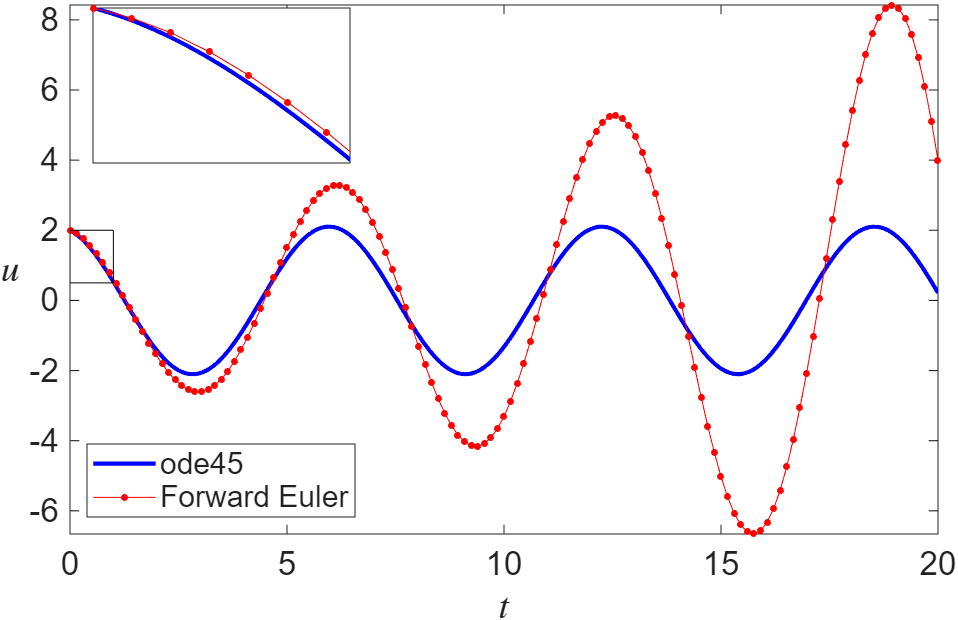
\includegraphics[width=0.7\linewidth,height=\textheight,keepaspectratio]{im/Forward_Euler_SHO.png}
\end{center}

The inset shows that the first few steps of the method match the
solution reasonably well. However, over time it appears that the error
builds up, and the amplitudes grow (despite the correct solution having
the same amplitude for all time). Reducing the timestep will improve
this, but eventually the amplitude will always begin to grow, at a rate
which will become approximately exponential.

We can see how this scheme behaves with the timestep more clearly by
considering the nonlinear van der Pol oscillator with \(C=3\), shown
below for four different choices of timestep \(\Delta t\):

\begin{center}
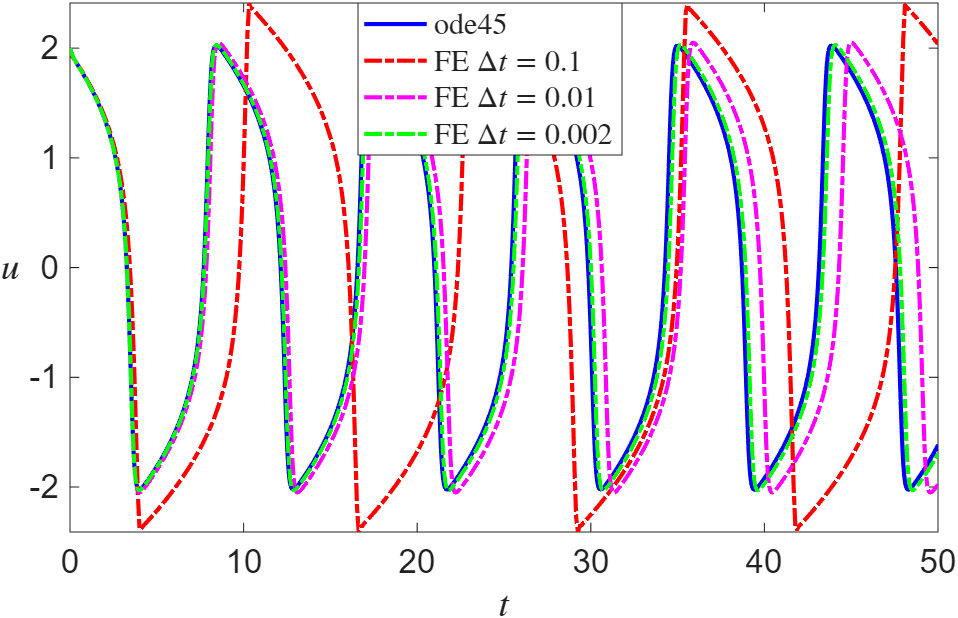
\includegraphics[width=0.7\linewidth,height=\textheight,keepaspectratio]{im/C3_FE_vanderPol.png}
\end{center}

We observe convergence towards a similar solution profile as
\(\Delta t\) decreases. However, there is still a buildup of error as
\(t\) increases, meaning that we will need to consider local errors over
one timestep, as well as global errors over iterative schemes for many
timesteps.

We can formalize these ideas in terms of the \textbf{local truncation
error (LTE),} which is essentially how much the approximation given in
the forward Euler method fails to exactly satisfy the ODE. We can
compute this by substituting in the true solution, \(\mathbf{u}(t)\),
and using Taylor series expansions to determine the error.

\phantomsection\label{eg-5.2}
\begin{fbxSimple}{eg}{Example 5.2}{}
\phantomsection\label{eg-5.2}
\textbf{LTE of forward Euler}

Expanding \(\mathbf{u}(t)\) in a Taylor series, we find: \[
\mathbf{u}_{n+1} = \mathbf{u}(t+\Delta t) = \mathbf{u}(t) + \Delta t \frac{\mathrm{d}\mathbf{u}}{\mathrm{d}t} + O(\Delta t^2) = \mathbf{u}_n + \Delta t \mathbf{f}(\mathbf{u}_n),
\] which implies that this method has an LTE of \(O(\Delta t^2)\). Note,
however, that we can do precisely the same calculation before
rearranging (via the approximation of the derivative directly) as: \[
\frac{\mathbf{u}_{n+1} - \mathbf{u}_n}{\Delta t} = \frac{\mathbf{u}(t+\Delta t) - \mathbf{u}(t)}{\Delta t} = \frac{\mathrm{d}\mathbf{u}}{\mathrm{d}t} + O(\Delta t) = \mathbf{f}(\mathbf{u}(t)),
\] which implies an LTE of \(O(\Delta t)\). These two definitions are
both used, despite being somewhat inconsistent. We will adopt the former
definition, which is sometimes called the \textbf{single-step error.}

\end{fbxSimple}

An integration scheme which has an LTE of the form \(O(\Delta t)\) or
smaller is called \textbf{consistent.} Essentially, a consistent scheme
is one where the approximations are equivalent to a collection of Taylor
series approximations, and hence, subject to various smoothness
assumptions, we expect to be able to make the error tend to \(0\) for
small enough time steps. However, consistency is not enough to ensure
that a numerical scheme converges to the analytical solution of the
original ODE.




\end{document}
